\documentclass[11pt,openany]{book}
\usepackage{geometry}
\geometry{
	letterpaper,
	margin=1in
}
\usepackage{blindtext}
\usepackage{tikz,tcolorbox}
\usepackage{pgfplots}
\usepackage{xcolor}
\usepackage{amsfonts}
\usepackage{hyperref} 
\usepackage{indentfirst}
\usepackage{graphicx}
\usepackage{caption}
\usepackage{subcaption}
\usepackage[normalem]{ulem}
\usepackage [english]{babel}
\usepackage [autostyle, english = american]{csquotes}
\usepackage{appendix}

\usepackage[ruled,linesnumbered]{algorithm2e}
\SetKwComment{Comment}{/* }{ */}
\DontPrintSemicolon 
\usepackage{tabularx}
\usepackage{amsmath,amssymb}
\usepackage{mathtools}
\usepackage{makecell}
\graphicspath{ {./images/} }
\usepackage{enumitem}
\usepackage{soul}
\usepackage{mathtools}
\usepackage{wrapfig}
\usepackage{mathrsfs}
\usepackage{centernot}
\usepackage{amsthm}
\usepackage{listings}
%\usepackage{biblatex}
%\addbibresource{bibliograph.bib}
\usepackage{microtype}
\usepackage{pagenote}
\usepackage{array}

\definecolor{codegreen}{rgb}{0,0.6,0}
\definecolor{codegray}{rgb}{0.5,0.5,0.5}
\definecolor{codepurple}{rgb}{0.58,0,0.82}
\definecolor{backcolour}{rgb}{0.95,0.95,0.92}

\lstdefinestyle{mystyle}{
	backgroundcolor=\color{backcolour},   
	commentstyle=\color{codegreen},
	keywordstyle=\color{magenta},
	numberstyle=\tiny\color{codegray},
	stringstyle=\color{codepurple},
	basicstyle=\ttfamily\footnotesize,
	breakatwhitespace=false,         
	breaklines=true,                 
	captionpos=b,                    
	keepspaces=true,                 
	numbers=left,                    
	numbersep=5pt,                  
	showspaces=false,                
	showstringspaces=false,
	showtabs=false,                  
	tabsize=2
}

\lstset{style=mystyle}
%% End notes to be printed as sections at the
%% end of each chapter.
\renewcommand*{\notedivision}{\section*{\notesname}}
\renewcommand*{\pagenotesubhead}[1]{}

%\newcommand*{\exercises}{\section*{\exercisename}}
%%%%%%%%%%%%% For customising the endnote markers. Comment these out if you don't want them.
% To prefix each note number with the chapter number
\renewcommand{\thepagenote}{\thechapter-\arabic{pagenote}}

% To have a slightly different formatting for the endnote numbers in the text -- smaller text, sans-serif, square brackets
\renewcommand\notenumintext[1]{\space{\footnotesize\sffamily[FN-#1]}}

% To have a slightly different formatting for the endnote numbers in the notes section. Just the square brackets and sans-serif; normal size.
\renewcommand\notenuminnotes[1]{{\sffamily[FN-#1] }}
% If you want a different name/heading for the end notes
\renewcommand{\notesname}{End Notes}
\newcommand{\exercisename}{Exercises}
\newcounter{thatonetheorem}
\newcounter{exercisecounter} % continuity of exercises in a section
\newenvironment{exerciselist}{
	\begin{enumerate}
		\setcounter{enumi}{\value{exercisecounter}}
	}{
		\setcounter{exercisecounter}{\value{enumi}}
	\end{enumerate}
}
\newenvironment{thatonethmlist}{
	\begin{enumerate}
		\setcounter{enumi}{\value{thatonetheorem}}
	}{
		\setcounter{thatonetheorem}{\value{enumi}}
	\end{enumerate}
}
\newcommand*{\exercises}{\section*{\exercisename}}

\newcommand\todo{\textcolor{red}{\textbf{TODO: }}}
%%%%%%%%%%%%% End customisation
\newcommand{\reals}{\mathbb{R}}
\newcommand\defeq{\mathrel{\stackrel{\makebox[0pt]{\mbox{\normalfont\tiny def}}}{=}}}
\makeatletter
\renewcommand*\env@matrix[1][*\c@MaxMatrixCols c]{%
  \hskip -\arraycolsep
  \let\@ifnextchar\new@ifnextchar
  \array{#1}}
\makeatother

\newcounter{thmcounter} % continuity of theorem
\newcommand{\definition}[2]{\begin{tcolorbox}[title=Definition {\thechapter}.{\arabic{thmcounter}} ({#1}),colframe=black,label={def:\thechapter.\thethmcounter}]
		{#2}\end{tcolorbox}

\addtocounter{thmcounter}{1}
}
\newcommand{\proposition}[1]{\begin{tcolorbox}[title=Proposition {\thechapter}.{\arabic{thmcounter}},colframe=red!50!blue!20!white,colback=red!35!blue!10!white, coltitle=black,label={prop:\thechapter.\thethmcounter}]{#1}\end{tcolorbox}
\addtocounter{thmcounter}{1}
}
\newcommand{\theorem}[2]{\begin{tcolorbox}[title=\color{black}Theorem {\thechapter}.{\arabic{thmcounter}} ({#1}),colframe=red!40,colback=red!5!white,label={thm:\thechapter.\thethmcounter}]{#2}\end{tcolorbox}
	
	\addtocounter{thmcounter}{1}
}
\newcommand{\example}[1]{\begin{tcolorbox}[title=Example {\thechapter}.{\arabic{thmcounter}},colframe=yellow!20!white,colback=yellow!10!white,coltitle=black,label={ex:\thechapter.\thethmcounter}]{#1}\end{tcolorbox}

\addtocounter{thmcounter}{1}
}
\newcommand{\corollary}[1]{\begin{tcolorbox}[]{Corollary {\thechapter}.{\arabic{thmcounter}}: {#1}}\end{tcolorbox}
	
	\addtocounter{thmcounter}{1}
}
\newtheorem*{remark}{Remark}
\newtheorem*{notation}{Notation}
%\newcommand{\exercises}{\section*{\exercisename}}
%% THIS LINE IS MANDATORY
\makepagenote

\begin{document}
	\tableofcontents
	% sample chapter
	\iffalse
	\chapter*{Sample chapter}
	\setcounter{thmcounter}{1}
	\section*{Section}
	This is a sample chapter structure.\\
	\definition{Real numbers}{
		We denote $\mathbb{R}$ as the set of real numbers. Intuitively, this set contains all the "decimals" including the non-terminating ones.
	}
	\theorem{Cantor}{
		The cardinality $|\mathbb{R}|$ is larger than $|\mathbb{Z}|$.
	}
	\begin{proof}
		Left as an exercise.
	\end{proof}
	\corollary{
		There is no bijective function mapping $\mathbb{Q}$ to $\mathbb{R}$.
	}
	\begin{proof}
		There is a bijective function from $\mathbb{Z}$ to $\mathbb{Q}$.
	\end{proof}
	\example{
		$1.3$ is a real number. So we say $1.3 \in \mathbb{R}$. \\
		$\pi$ is a real number. So we say $\pi \in \mathbb{R}$.
	}

	\exercisename

	\begin{enumerate}
		\item Show that all the zeros of $\zeta(s)$ lie on the line $\Re (z)=1/2$.
	\end{enumerate}
	\fi
	%\chapter{Coordinate Geometry}
\setcounter{exercisecounter}{0}

\setcounter{thmcounter}{0}
\section{Introduction}
Many of you have encountered some form of coordinate geometry in high school. For instance, the ``standard" way to visualize a graph e.g. $f(x)=x^2$ is to visualize the points in 2-D space $(x,y)$ where $y=x^2$. We give a demonstration in Python code.

\begin{lstlisting}[language=Python]
import matplotlib.pyplot as plt
import numpy as np
X=np.arange(-100,100) #create list of numbers from -100 to 100
Y= X**2 #calculate the square of at each x
plt.plot(X,Y) #plot all the pairs of points in 2d plane
plt.xlabel('x')
plt.ylabel('y=x^2')
plt.title('Visualization of the "object"')
plt.show()
plt.show()
\end{lstlisting}
\begin{tikzpicture}
	\node (A) at (0,0) {$x$};
	\node (B) at (3,0) {$x^2$};
	\draw[->,thick]
	(A)--(B)
	node[midway,below] {the ``graph" object} ;
	\node(whitehead) at (8,0){
		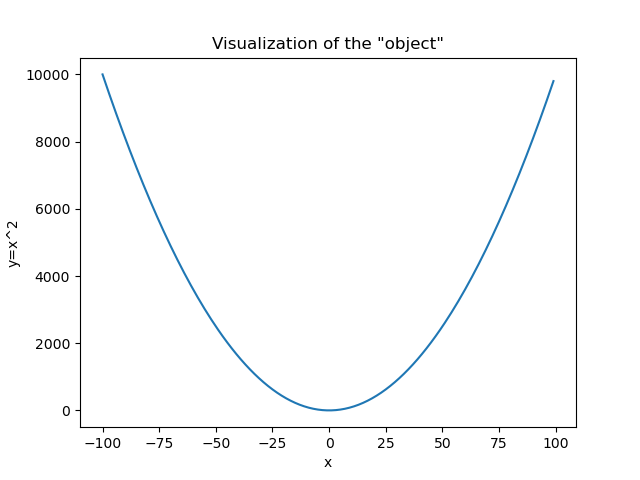
\includegraphics[width=0.6\textwidth]{coordinate_geometry/square_graph.png}
	};
\end{tikzpicture}


This is also known as the Cartesian plane, named after René Descartes who invented it in the 17th century.\\
\section{Visualization of geometric objects}

The Cartesian plane allows us to describe shapes with equations and perform calculations with them. We first define the playing field (the Cartesian plane and higher dimensional analogues) and the players.
\definition{Real numbers}{
	The set of \textbf{real numbers}, denoted as $\mathbb{R}$, is (informally) the set of all the numbers that can be written out in decimal form.
}
\example{
The following are real numbers:
\begin{enumerate}
	\item The integers $0$, $\pm 1$, $\pm 2$, ...  
	\item Fractions in the form $\frac{a}{b}$, where $a$ and $b\neq 0$ are integers.
	\item Irrational numbers $\sqrt{2}$, $\pi$.
\end{enumerate}
}
\begin{remark}
	The set of real numbers is known as a \textbf{complete field}. The definition of a complete field will be swept under the rug, but it guarantees a few things. The most important property: We will not ``escape" the set by performing operations, possibly infinitely many.
\end{remark}
\definition{N-dimensional space}{
	Let $n$ be a positive integer. We denote the \textbf{n-dimensional real space} to be $\mathbb{R}^n$, consisting of all the $n$-tuples $(x_1,x_2,x_3,...,x_n)$, where each $x_j$ is a real number. \\
	We call an $n$-tuple $(x_1,...,x_n)$ a \textbf{point}, and two points $(x_1,...,x_n)$ and $(y_1,...,y_n)$ are equal if $x_j=y_j$ for all $j$-th entries of the tuples.
}
\begin{remark}
	We sometimes use $\mathbf{x}$ to denote $(x_1,...,x_n)$ to make notation cleaner.
\end{remark}
\subsection{Lines}
Now that we have introduced the playing field of n-dimensional space, we can start translating the axioms of euclidean geometry to this coordinate system.
\definition{Lines}{
	In euclidean geometry, a line is defined by two points. We let $\mathbf{x},\mathbf{y} \in \mathbb{R}^n$. The \textbf{line} going from $\mathbf{x}$ to $\mathbf{y}$ is denoted $\overrightarrow{\mathbf{xy}}$.
}
What would this line look like? To get from $\mathbf{x}$ to $\mathbf{y}$, we have to traverse $y_1-x_1$ units in the first coordinate, $y_2-x_2$ units in the second, ..., $y_n-x_n$ in the last. We thus have a natural notation for the line $\overrightarrow{\mathbf{xy}}$.
\[
 \overrightarrow{\mathbf{xy}}=(y_1-x_1,y_2-x_2,...,y_n-x_n).
\]

This is very similar to a point as an n-tuple, but this is ``spiritually" different to a point. This tuple represents the direction of line. One way to think of the correspondence between $(x_1,...,x_n)$ point and $(x_1,...,x_n)$ line is that $(x_1,...,x_n)$ line is the line connecting $(0,0,...0)$ to $(x_1,...,x_n)$ point. Because of this, we can identify a tuple as both the point and the line, and we call it a ``vector" to abstract away from the actual geometric meaning.
\begin{figure}[h]
	\centering
	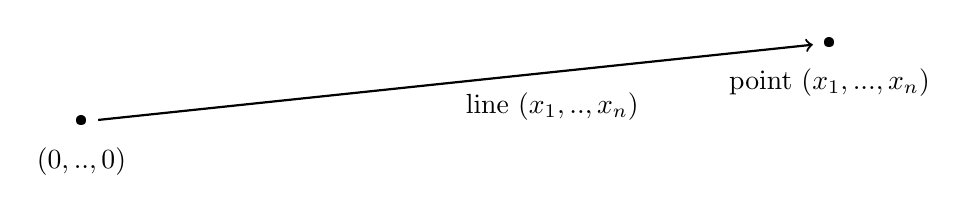
\begin{tikzpicture}[node distance=2cm]
		\node (A)[draw=none,label=below:{$(0,..,0)$}] at (0,0) {\textbullet};
		\node (B)[draw=none,label=below:{point $(x_1,...,x_n)$}] at (9.5,1) {\textbullet};
		
		\draw[thick, ->]
		(A) -- (B) 
		node[midway, below right] {line $(x_1,..,x_n)$};
	\end{tikzpicture}
	\caption{The correspondence between a line ``vector'' and a point ``vector''.}
\end{figure}

\begin{notation}
	Vectors are a very general notation of $n-tuples$. Depending on context, we use both of the following notations to denote the entries of $\vec{v}\in\reals^n$ \begin{itemize}
		\item ``Ordered sets'' $(v_1,...,v_n)$, suitable dealing with points (and other geometric objects). It also looks cleaner when writing inline.
		\item ``Column vectors'' $\begin{bmatrix}
			v_1\\.\\.\\.\\v_n
		\end{bmatrix}$ when the ordered sets are complicated to read, and when working with matrix algebra.
	\end{itemize}
\end{notation}
\subsection{Operation with lines}
We need to translate a few more things from euclidean geometry.

\proposition{
Let $\mathbf{x}, \mathbf{y}, \mathbf{z} \in \mathbb{R}^n$, then \[
	\overrightarrow{\mathbf{xy}}+\overrightarrow{\mathbf{yz}}=\overrightarrow{\mathbf{xz}},
\]
where $(a_1,...,a_n)+(b_1,...,b_n)\defeq(a_1+b_1,..., a_n+b_n)$.
}
\begin{proof}
	\begin{align*}
		\overrightarrow{\mathbf{xy}}+\overrightarrow{\mathbf{yz}}&=(y_1-x_1,..., y_1-x_n)+(z_1-y_1,..., z_1-y_n)\\
		&=(y_1-x_1+z_1-y_1, ... ,y_n-x_n+z_n-y_n)\\
		&= (z_1-x_1, ...,z_n-x_n)\\
		&= \overrightarrow{\mathbf{xz}}
	\end{align*}
\end{proof}
\

Geometrically, this means if you connect $\mathbf{x}$ to $\mathbf{y}$ to $\mathbf{z}$, the overall ``direction of travel" you make is $\mathbf{x}$ to $\mathbf{z}$. This gives us a natural extension for addition of vectors by considering each entry. Similarly for scaling vectors, we just scale the entries along each dimension.

 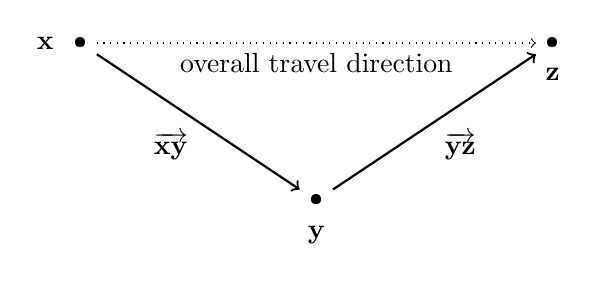
\begin{tikzpicture}[node distance=2cm]
 	\node (A)[draw=none,label=left:$\mathbf{x}$] at (0,0) {\textbullet};
 	\node (B)[draw=none,label=below:$\mathbf{y}$] at (3,-2) {\textbullet};
 	\node (C)[draw=none,label=below:$\mathbf{z}$] at (6,0) {\textbullet};
 
 	\draw[thick, ->]
 	(A) -- (B)
 	node[midway, below left]{$\overrightarrow{\mathbf{xy}}$};
 	\draw[thick, ->]
 	(B) -- (C)
 	node[midway, below right]{$\overrightarrow{\mathbf{yz}}$};
 	
 	\draw[dotted,->]
 	(A)--(C)
 	node[midway, below] {overall travel direction};
 	
 \end{tikzpicture}\ \\

\definition{Addition and scaling of vectors}{
	Let $\vec{a},\vec{b}$ be two vectors in $\mathbb{R}^n$. We define the sum/difference of $\vec{a}$ and $\vec{b}$ \[
		\vec{a}+\vec{b} \defeq (a_1+b_1,...,a_n+b_n), \quad \vec{a}-\vec{b} \defeq (a_1-b_1,...,a_n-b_n)
	\] and the scaling of $\vec{a}$ by a real number $c\in \mathbb{R}$ \[
		c\vec{a} \defeq (c a_1, c a_2,... ,c a_n).
	\]
}
\begin{remark}
	Here we use the term ``vectors", as we can in essence add points and lines together. How does one make sense of adding a line to a point? We can view this as translating the point along the path of the line, for instance, let us translate the point $(1,2)$ $3$ units in the first coordinate and $-1$ units in the second coordinate. This will give us $(4,1)$.
	
	\begin{figure}[h]
		\centering
		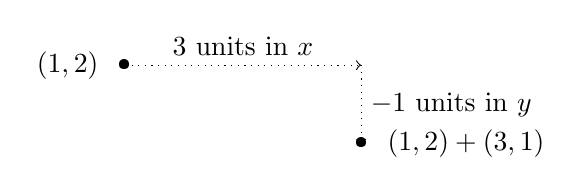
\begin{tikzpicture}[node distance=2cm]
			\node (A)[draw=none,label=left:{$(1,2)$}] at (1,2) {\textbullet};
			\node (y)[draw=none, label=right:{$(1,2)+(3,1)$}] at (4,1){\textbullet};
			\draw[->,dotted]
			(1,2)--(4,2)
			node [midway, above]{$3$ units in $x$};
			
			\draw[->, dotted]
			(4,2)--(4,1) node [midway,right]{$-1$ units in $y$};
		\end{tikzpicture}
	\end{figure}
\end{remark}

This way, we can write the line from $\vec{x}$ to $\vec{y}$ as $\vec{y}-\vec{x}$. The proof is a computational exercise. \\ 
\begin{notation}
	We now transferred for talking about points and the lines between points to addition. Therefore, we can overload the notation for points and lines as a vector $\vec{v}$, keeping in mind that they have the same arithmetic structure.
\end{notation}


In fact, most of our intuition for the real numbers translates to $\mathbb{R}$. For formality, we will list them here; in practice, we (almost always) take these properties for granted.
\proposition[vectorspace]{
	Let $\vec{u},\vec{v},\vec{w} \in \mathbb{R}^n$, and $a,b \in \mathbb{R}$. Then the following hold:
	\begin{itemize}
		\item \textit{(Associativity)} $(\vec{u}+\vec{v})+\vec{w} = \vec{u}+(\vec{v}+\vec{w})$.
		\item \textit{(Commutativity)} $\vec{u}+\vec{v} = \vec{v}+\vec{u}$.
		\item \textit{(Identity)} The zero vector $\vec{0}\defeq (0,0,...,0)\in\reals$ satisfies $\vec{v}+\vec{0}=\vec{v}$.
		\item \textit{(Inverse)} The inverse of $\vec{v}$, $-\vec{v}\defeq(-v_1,...,-v_n)$ satisfies $\vec{v}+(-\vec{v})=\vec{0}$.
		\item \textit{(Scalar multiplication)} $a(b\vec{v})=(ab)\vec{v}$.
		\item \textit{(Scalar Identity)} $1\vec{v}=\vec{v}$.
		\item \textit{(Distributivity 1)}  $a(\vec{u}+\vec{v})=a\vec{u}+a\vec{v}$.
		\item \textit{(Distributivity 2)}  $(a+b)\vec{v}=a\vec{v}+b\vec{v}$.
	\end{itemize}
} 
\begin{remark}
	All of these have good geometric intuition behind. For instance, the zero vector $\vec{0}$ is the ``don't move" vector, corresponding to the point at the origin, or the ``too short to be a line''. The inverse of $\overrightarrow{\mathbf{xy}}$ is $\overrightarrow{\mathbf{yx}}$, where you go back from $\mathbf{x}$ to $\mathbf{y}$. \begin{tikzpicture}
		
	\end{tikzpicture}
\end{remark}
\begin{remark}
	These $8$ conditions are the axioms of a vector space. Later in the course, we will generalize the notion of vectors in $\reals^n$ to other spaces (playing fields).
\end{remark}
\proposition{
	Lines are translation invariant. That is, for every $\vec{x},\vec{y},\vec{v}\in\mathbb{R}^n$, then the 
	line from $\vec{x}$ to $\vec{y}$ is the same as the line from $\vec{x}+\vec{v}$ to $\vec{y}+\vec{v}$.
}
Let us illustrate what this statement is trying to convey. We have two points $\vec{x}$, $\vec{y}$; now we translate each of these points by $\vec{v}$, and we want the line between the points to be preserved under this translation.\\
\begin{tikzpicture}
	\node (X)[draw=none,label=left:$\vec{x}$] at (0,0) {\textbullet};
	\node (Y)[draw=none,label=below:$\vec{y}$] at (5,-1) {\textbullet};
	\node (XT)[draw=none,label=below:$\vec{x}+\vec{v}$] at (-2,-2) {\textbullet};
	\node (YT)[draw=none,label=below:$\vec{y}+\vec{v}$] at (3,-3) {\textbullet};
	
	\draw[->,thick] 
	(X)--(Y)
	node (a)[midway, above right] {$\vec{y}-\vec{x}$};
	
	\draw[->,dotted] 
	(X)--(XT)
	node[midway, above left] {$\vec{v}$};
	
	\draw[->,dotted] 
	(Y)--(YT)
	node[midway, above left] {$\vec{v}$};
	
	
	\draw[->,color=blue] 
	(XT)--(YT)
	node[midway, below left] {?};
\end{tikzpicture} \ \\
The proof is one line: $(\vec{y}+\vec{v}) - (\vec{y}+\vec{v}) = \vec{y}-\vec{x} +\vec{v}-\vec{v}=\vec{y}-\vec{x}$. However, an immediate consequence of this is that we can ``transport'' vectors in space without distorting the vector. Colloquially, \textit{5 miles South} to you describes the same direction and length as \textit{5 miles South} to a person a few feet away. This justifies the way we visualize the correspondence between points and vectors - we ``transport'' the vectors to start from the origin $(0,...,0)$, and the end describes the point.

\begin{remark}
	Translation (and scaling) invariance is a property of Euclidean geometry. There are some exotic geometry systems that distort distance and direction through translation and scaling. One such example is the Poincar\'e metric.
\end{remark}
Another notion we can carry from Euclidean geometry is parallel lines. Here we not only define what it means for two vectors to be parallel (never touching), we also give a definition for two vectors to be parallel but point in opposite directions.
\definition{Parallel and Antiparallel Vectors}{
	Let non-zero vectors $\vec{v},\vec{w}\in\reals^n$.
	We say that $\vec{v}$ and $\vec{w}$ are \textbf{parallel} if there is some $c>0$ such that $\vec{v}=c\vec{w}$. We say that $\vec{v}$ and $\vec{w}$ are \textbf{antiparallel} if there is some $c<0$ such that $\vec{v}=c\vec{w}$.
}
\example{
	Find an expression for the points on the (infinite) line passing through $P(1,1,0)$ and $Q(0,2,2)$.
}
Let $M$ be a point on the line $\overrightarrow{PQ}$, then $\overrightarrow{PM}$ is parallel to $\overrightarrow{PQ}$ (or $M=P$). Either way, we would have some $c\in\reals$ such that \[
\overrightarrow{PM}=c\overrightarrow{PQ}.
\]
Indeed, we can confirm that any point represented as $P+c\overrightarrow{PQ}$ will be on the line, as $c\overrightarrow{PQ}$ is parallel to $\overrightarrow{PQ}$. One exception is to check for when $c=0$, but we already know $P$ is on the line.
We thus have an expression for the line to be \[
	(1,1,0) + c(-1,1,2)
\]
for all $c\in\reals$. Another way to put it, the line is the \textbf{image} of the function $f(c) = (1,1,0) + c(-1,1,2)$ on $\reals$.
\begin{remark}
	This form of representing a line is known as a \textbf{parametric representation} or a \textbf{parametrization} of the line. We will give a more concrete definition of parametrization when we move beyond straight lines to ``curvy'' curves and surfaces in \ref{noideayet}.
\end{remark}
\begin{remark}
	Using the parametric representation for a line $l(t) = (P_1,P_2,...,P_n)+ t(v_1,v_2,...,v_n)$, we can take slices/cross sections across each of the $j$-th coordinates, and get \[
	x_j = P_j+tv_j \implies t = \frac{x_j-P_j}{v_j}
	\] 
	is the equation of a line in 2d. $P_j, v_j$ are fixed, viewing in the variables $y=x_j, x=t$, this is the equation of a line with y-intercept $x_j$ and slope $v_j$. Setting the values of t for all slices to be equal, \[
	t= \frac{x_1-P_1}{v_1}=\frac{x_2-P_2}{v_2}=...=\frac{x_j-P_j}{v_j}=...=\frac{x_n-P_n}{v_n}
	\]
	This form is known as the \textbf{symmetric equations} of a line.
\end{remark}

\example{
	Find an expression for the points on the line connecting \textbf{between} $P(1,1,0)$ to $Q(0,2,2)$.
}
This will be a segment of the line from the previous example, so the answer would be the same expression, but we limit the domain of $f$ to be an interval on $\reals$. Let us examine what $f$ does to a few values of $c$.
\renewcommand{\arraystretch}{1.5}
\begin{center}
	\begin{tabular}{|c|c c c c c|} 
		\hline
		c & very negative & $c=0$ & $c=1/2$& $c=1$ & very positive \\ 
		\hline
		f(c) & very off the segment & $P$ & midpoint of $\overline{PQ}$& $Q$ & very off the segment \\ 
		\hline
	\end{tabular}
\end{center}
As we move from very negative $c$ to very positive $c$, we start very away from the line segment, reach $P$ at $c=0$, $Q$ at $c=1$, then move away from the line segment. 
Indeed the values $(1,1,0) + c(-1,1,2)$ will be on the line segment for $c\in[0,1]$.

%
Finally, the nice algebraic properties for adding and scaling vectors gives us a natural way to understand these vectors as a sum of $n$ component vectors, one for each dimension. These \textit{special} vectors deserve a name.
\definition{Standard Basis Vectors and Vector Decomposition}{
	We denote in $\reals^n$, the \textbf{standard basis vectors} \begin{align*}
		\vec{e}_1 &\defeq (1,0,0,...,0,0,0),\\
		\vec{e}_2 &\defeq (0,1,0,...,0,0,0),\\
		\vec{e}_{n-1}&\defeq (0,0,0,...,0,1,0),\\
		\vec{e}_n&\defeq(0,0,0,...,0,0,1),
	\end{align*}
	so that $\vec{v}=\sum_{i=1}^n v_i \vec{e}_i$.
	In $\reals^3$, we sometimes write \[
		\vec{i}\defeq \vec{e}_1, \quad \vec{j}\defeq \vec{e}_2,\quad \vec{k}\defeq\vec{e}_3
	\]to accommodate the physicists.
}\ \\
\exercises
\begin{exerciselist}
	\item Compute $5\vec{v}-2\vec{w}$ and $-3\vec{w}$ for the following pairs of vectors: \begin{enumerate}[label=(\alph*)]
		\item $\vec{v}=2\vec{i}+3\vec{j}$, $\vec{w}=4\vec{i}-9\vec{j}$
		\item $\vec{v}=(1,2,-1)$, $\vec{w}=(2,-1,0)$
		\item $\vec{v}=-2\vec{e}_3+4\vec{e}_5$, $\vec{w}=\vec{e}_1 -4\vec{e}_5$
		\item $\vec{v}=(\cos t, \sin t)$, $\vec{w}=(\cos t)\vec{e}_2 - (\sin t) \vec{e}_1$
	\end{enumerate}
	
	\item Find parametric equations that describe the line that \begin{enumerate}[label=(\alph*)]
		\item passes through $(1,2,3)$ and $(4,-1,2)$
		\item passes through $(0,-2,3)$ and $(1,2,3)$
	\end{enumerate}
\end{exerciselist}
\section{Length, angles and projections}
\definition{Magnitude}{
Let $\vec{v}\in\reals^n$. The magnitude of $\vec{v}$ is denoted \[
|\vec{v}| \defeq \sqrt{v_1^2 + v_2 ^2+ ... v_n^2}.
\]
}
We build intuition through the lower dimensional cases.
In $\reals^2$, let us consider the point $(4,3)$.\\
\begin{wrapfigure}{r}{0.3\textwidth}
	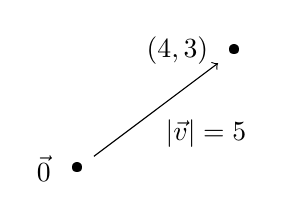
\begin{tikzpicture}
		\node (X)[draw=none,label=left:{$\vec{0}$}] at (0,0) {\textbullet};
		\node (Y)[draw=none,label=left:{$(4,3)$}] at (2,1.5) {\textbullet};
		\draw[->]
		(X)--(Y)
		node [midway, below right] {$|\vec{v}|=5$};
	\end{tikzpicture}
\end{wrapfigure}

The magnitude of this vector is $\sqrt{3^2+4^2}=5$. If this sounds very familiar, it is because this is indeed an application of Pythagorean theorem. In 3-dimensions, this still applies - take $\vec{x}=(a,b,c)$, we can traverse in each coordinate to apply Pythagorean theorem twice.

\usetikzlibrary {3d}

\begin{figure}[h]
	\centering
	\begin{subfigure}{0.3\textwidth}
		\centering
		\begin{tikzpicture}
			
			\draw[->](0,0,0) -- (xyz cylindrical cs:radius=3);
			\node at (3.5,0,0){$x_1$};
			\draw[->] (0,0,0) -- (xyz cylindrical cs:radius=3,angle=90);
			\node at (0,3.5,0){$x_2$};
			\draw[->] (0,0,0) -- (xyz cylindrical cs:z=3);
			\node at (0,0,3.5){$x_3$};
			\draw[->,dotted,thick,color=red] (0,0,0) -- (2,0,0)
			node[midway,below]{a};
			\draw[->,dotted,thick,color=red] (2,0,0) -- (2,3,0) node[midway,right]{b};
			\draw[->,dotted,thick,color=red] (2,3,0) -- (2,3,1)
			node[midway,above]{c};
			\draw[->,color=blue] 
			(0,0,0) -- (2,3,1)
			node[midway, below]{$\vec{x}$};
		\end{tikzpicture}
		\caption{$\vec{x}=(a,b,c)$.}
	\end{subfigure}
	\begin{subfigure}{0.3\textwidth}
		\centering
		\begin{tikzpicture}
			
			\draw[->](0,0,0) -- (xyz cylindrical cs:radius=3);
			\node at (3.5,0,0){$x_1$};
			\draw[->] (0,0,0) -- (xyz cylindrical cs:radius=3,angle=90);
			\node at (0,3.5,0){$x_2$};
			\draw[->] (0,0,0) -- (xyz cylindrical cs:z=3);
			\node at (0,0,3.5){$x_3$};
			\draw[->,dotted,thick,color=red] (0,0,0) -- (2,0,0)
			node[midway,below]{a};
			\draw[->,dotted,thick,color=red] (2,0,0) -- (2,3,0) node[midway,right]{b};
			\draw[->,color=brown] 
			(0,0,0) -- (2,3,0)
			node[midway, left]{$\sqrt{a^2+b^2}$};
			
		\end{tikzpicture}
		\caption{Pyth. thm on $a,b$.}
	\end{subfigure}
	\begin{subfigure}{0.3\textwidth}
		\centering
		\begin{tikzpicture}
			[z={(10:10mm)},x={(-45:5mm)}]
			
			\draw[->](0,0,0) -- (3,0,0);
			\node at (3.5,0,0){$x_1$};
			\draw[->] (0,0,0) -- (0,3,0);
			\node at (0,3.5,0){$x_2$};
			\draw[->] (0,0,0) -- (0,0,-3);
			\node at (0,0,-3.5){$x_3$};
			\draw[->,color=brown] 
			(0,0,0) -- (2,3,0)
			node[midway, right]{$\sqrt{a^2+b^2}$};
			
			\draw[->,dotted,thick,color=red] (2,3,0) -- (2,3,-1) node[midway, above]{c};
			\draw[->,color=blue] 
			(0,0,0) -- (2,3,-1)
			node[midway, left]{$\sqrt{a^2+b^2+c^2}$};
			
		\end{tikzpicture}
		\caption{Reapply Pyth. thm.}
	\end{subfigure}
	
\end{figure}\ \\

\proposition{
	Let $\vec{v} \in \reals^n, a\in\reals$. Then \[
	|a\vec{v}| = |a||\vec{v}|.
	\]
}\ \\
\definition{Unit vector}{
	Let $\vec{v}\in\reals^n$. We call $\vec{v}$ a \textbf{unit vector} if $|\vec{v}|=1$.
}
\proposition{
	Let $\vec{v}\in\reals^n$ be non-zero. Then there is a unique unit vector $|\vec{w}|=1$ such that $\vec{v}$ is parallel to $\vec{w}$.
}
\begin{proof}
	If $|\vec{w}|=1, c>0$ and $c\vec{w}=\vec{v}$, it must be that \[
		c = |c||\vec{w}| = |c\vec{w}| = |\vec{v}|,
	\]
	and \[
		\vec{w} = \frac{1}{c}(c\vec{w}) = \frac{1}{|vec{v}|}\vec{v}.
	\] This shows uniqueness - there is no other possible candidate except for this vector. Now we can confirm the vector $\frac{1}{|\vec{v}|}\vec{v}$ is a unit vector and is parallel to $\vec{v}$, so there exists a unique unit vector that satisfies the properties.
	\\
\end{proof}
We have now transported the notions of length and scaling into the coordinate system, and this allows us to make ``measurements'' such as angles and area.

\subsection{The Dot Product}
\example{
Let points A=$(5,8)$, B=$(-2, 7)$, O=$(4,5)$. Find the angle $\angle AOB$.
}
To solve this using only information about the lengths, recall the Law of Cosines:

\theorem{Law of Cosines}{
For any triangle 
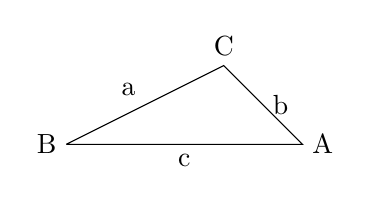
\begin{tikzpicture}
	
	\draw (0,0) node [left] {B}--(2,1) node [above]{C} node [midway, above left]{a}--(3,0) node [right]{A} node [midway, right]{b}--(0,0)node [midway, below]{c};
	%pic["$\alpha$",draw=orange,<->,angle eccentricity=1.2,angle radius=1cm] {angle=(0,0)--(2,1)--(3,0)};
\end{tikzpicture},
\[
	c^2 = a^2+b^2 - 2 a b \cos(\angle BCA).
\]
}

We now apply the Law of Cosines to $\triangle AOB$, so that\[
	|\overrightarrow{AO}|^2  +|\overrightarrow{OB}|^2- 2 |\overrightarrow{AO}| |\overrightarrow{OB} \ |\cos(\angle AOB) = |\overrightarrow{AB}|^2.
\]
Plugging in the values, we solve 
\begin{align*}
		((4-5)^2 + (5-8)^2) + ((-2-4)^2+(7-5)^2) - 2 \sqrt{(4-5)^2 + (5-8)^2} \\ \times \sqrt{(-2-4)^2+(7-5)^2} \cos(\angle AOB) = ((-2-5)^2+(7-8)^2).
\end{align*}
Simplifying, we get\[
	50 - 2 \sqrt{10} \sqrt{40} \cos(\angle AOB) = 50 \implies \cos(\angle AOB) = 0.
\]
So the angle is $\pi/2$.

\example{
	Find a closed form formula for the cosine of an angle formed by two vectors $\vec{v},\vec{w} \in\reals^n$.
}
Let the angle formed be $\theta$. Using the intuition from 2-D space, we can form a triangle (in a very complex n-dimensional space). We write the Law of Cosine in terms of vectors
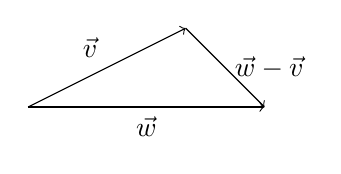
\begin{tikzpicture}
	
	\draw [->](0,0) -- (2,1) node [midway, above left]{$\vec{v}$};
	\draw [->](0,0)--(3,0) node [midway, below]{$\vec{w}$};
	\draw [->](2,1)--(3,0)node [midway, right]{$\vec{w}-\vec{v}$};
	%pic["$\alpha$",draw=orange,<->,angle eccentricity=1.2,angle radius=1cm] {angle=(0,0)--(2,1)--(3,0)};
\end{tikzpicture}
 \[
|\vec{v}|^2+|\vec{w}|^2-2|\vec{v}||\vec{w}|= |\vec{w}-\vec{v}|^2.
\]
This expands to \begin{align*}
	\sum_{i=1}^{n} v_i^2 + \sum_{j=1}^{n} w_j^2  - 2 \sqrt{\sum_{i=1}^{n} v_i^2}\sqrt{\sum_{j=1}^{n} w_j^2} \ \cos(\theta) =
	\sum_{i=1}^n (w_i-v_i)^2.
\end{align*}
Rearranging $(a-b)^2 = a^2+b^2-2ab$,
\[
2 \sqrt{\sum_{i=1}^{n} v_i^2}\sqrt{\sum_{j=1}^{n} w_j^2} \ \cos(\theta) = \sum_{i=1}^n 2 w_i v_i 
\]
so \[
\cos(\theta) = \frac{\sum_{i=1}^n w_i v_i }{\sqrt{\sum_{i=1}^{n} v_i^2}\sqrt{\sum_{j=1}^{n} w_j^2}}.
\]
\definition{Dot Product}{
	Let $\vec{v},\vec{w}\in\reals^n$, the \textbf{dot product} between $\vec{v}$ and $\vec{w}$ is \[
		\vec{v} \cdot \vec{w} \defeq \sum_{i=1}^n v_i w_i. 
	\]
}
\proposition{
Let $\vec{v}\in\reals^n$, then $|\vec{v}|^2 = \vec{v}\cdot\vec{v}$.
}
\proposition[1.22]{
	Let $\vec{u},\vec{v},\vec{w}\in\reals^n$, $c\in\reals$. The dot product satisfies the following properties:
	\begin{itemize}
		\item \textit{(Symmetry)} $\vec{v}\cdot\vec{w}=\vec{w}\cdot\vec{v}$.
		\item \textit{(Linearity 1)} $(c\vec{v})\cdot\vec{w} = c (\vec{v}\cdot\vec{w}) \textrm{(}= \vec{v}\cdot(c\vec{w})\textrm{  by symmetry)}$.
		\item \textit{(Linearity 2)} $(\vec{v}+\vec{u})\cdot\vec{w} = \vec{v}\cdot\vec{w}+\vec{u}\cdot\vec{w}$.
		\item \textit{(Positive definiteness)} $\vec{v} \cdot\vec{v}\geq0$, with equality if and only if $\vec{v}=\vec{0}$.
	\end{itemize}
}
\begin{proof}
	Here is the proof for the last property. The rest are left as an exercise We have $\vec{v}\cdot\vec{v} = |\vec{v}|^2\geq=0$, and if $\vec{v}\cdot\vec{v}=0$, for all $1\leq\j\leq n$, $v_j^2 \leq \sum_{i=1}^{n} v_i^2 = \vec{v}\cdot\vec{v}\leq0$, so $v_j=0$. This means $\vec{v}=\vec{0}$.
\end{proof}
\corollary[dotproduct]{
	
	\begin{enumerate}
		\item $
		|\vec{v}-\vec{w}|^2 = |\vec{v}|^2 + |\vec{w}|^2 - 2 \vec{v}\cdot\vec{w}.
		$
		\item In lower dimensions $\reals^2, \reals^3$ If $\vec{v},\vec{w}\neq \vec{0}$, the angle between $\vec{v}$ and $\vec{w}$ is\[
		\cos^{-1}\left(\frac{\vec{v}\cdot\vec{w}}{|\vec{v}||\vec{w}|}\right).
		\]
		In particular, the angle is $\pi/2$ when $\vec{v}\cdot\vec{w}=0$. 
		\item $|\vec{v}\cdot\vec{w}|\leq |\vec{v}||\vec{w}|.$
	\end{enumerate}
}

\theorem[cauchyschwarz]{Cauchy-Schwarz inequality}{
Let $\vec{v},\vec{u}\in\reals^n$. Then \[
	|\vec{v}\cdot\vec{u}|\leq |\vec{u}||\vec{v}|.
\]
}
The proof is in one of the exercises at the end of this chapter. \\
The dot product allows us to make sense of ``angles'' in higher dimensions, so we can generalize the notion of two vectors ``perpendicular'' to each other.
\definition{Orthogonality}{
Let $\vec{v},\vec{w}\in\reals^n$. We say $\vec{v}$ and $\vec{w}$ are \textbf{orthogonal} to each other if $\vec{v}\cdot\vec{w}=0$.
}

\example[1.26]{
	Find all vectors $\vec{v}\in\reals^3$ such that $\vec{v}\cdot(-3\vec{i}+2\vec{j}+6\vec{k}) =49$. Sketch the locus of corresponding points in $\reals^3$.
}

\label{plane_projection}
The condition expands to \begin{align*}
	-3v_1+2v_2+6v_3 &= 49 \\
	\implies v_3 &= \frac{49+3v_1 - 2v_2}{6}  
\end{align*}
so that the set of all vectors is \[
	\left\{s \vec{i}+t \vec{j}+\left(\frac{49+3s - 2t}{6}\right) \vec{k} | s,t\in\reals\right\}.
\]
To plot this in 3D space, notice that this describes the equation of a plane $z={(49+3x-2y)}/{6}$. We pick any three points (of course we want those that are easy to calculate) $(0,0,49/6)$, $(0,49/12,0)$, $(-49/18,0,0)$.
\iffalse
\begin{figure}
	\centering

	\subfloat%[\centering label 1]
	{{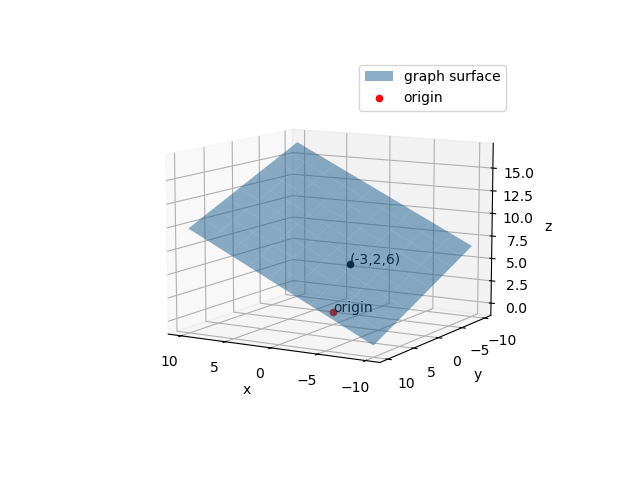
\includegraphics[width=7cm]{coordinate_geometry/plane1.png} }}%
	\qquad
	\subfloat%[\centering label 2]
	{{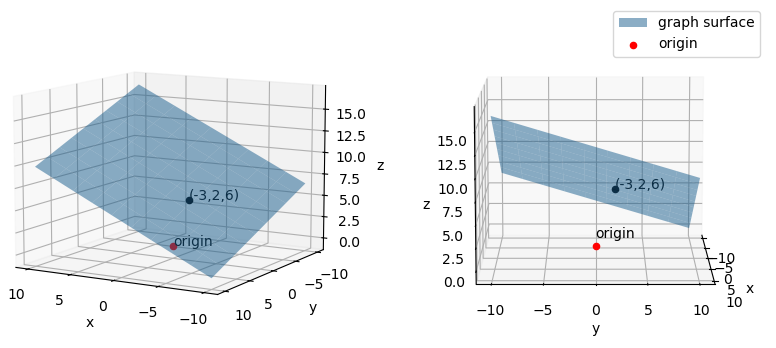
\includegraphics[width=7cm]{coordinate_geometry/plane2.png} }}%
	\caption{Two views of the plane}
\end{figure}
\fi
\begin{lstlisting}[language=Python]
	def function_to_plot(X,Y):
	return (49+3*X-2*Y)/6
	#create figure
	fig=plt.figure(figsize=(10,8))
	ax = fig.add_subplot(projection='3d')
	ax.view_init(elev=10, azim=120) #change view 1  
	#ax.view_init(elev=10, azim=0) #change view 2
	X,Y=np.meshgrid(np.linspace(-10,10,10), np.linspace(-10,10,10))
	Z=function_to_plot(X,Y)
	surface=ax.plot_surface(X, Y, Z, alpha=0.5,
	label='graph surface')
	ax.set_xlabel('x')
	ax.set_ylabel('y')
	ax.set_zlabel('z')
	#plot the curve and the cross section to integrate
	ax.scatter(0,0,0,color='red',label='origin')
	ax.text(0,0,0,'origin')
	ax.scatter(-3,2,6,color='black')
	ax.text(-3,2,6,'(-3,2,6)')
	plt.legend()
	plt.show()
\end{lstlisting}

\begin{figure}[h]
	\centering
	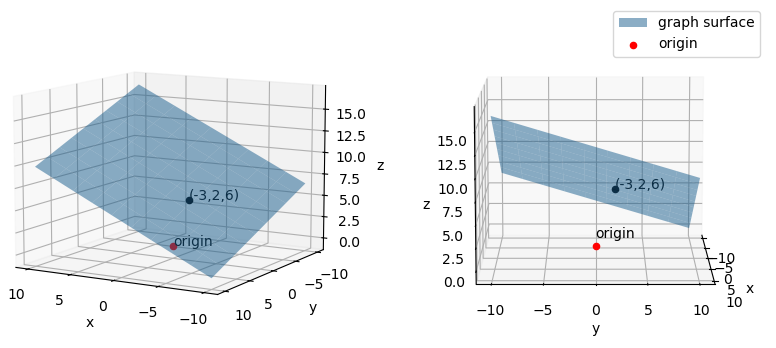
\includegraphics[width=\textwidth]{coordinate_geometry/plane2.png}
	\caption{Two views of the plane}
\end{figure}\ \\

Interestingly, we see that $(-3,2,6)$ - the point corresponding to our vector - is a point on the plane!
\begin{remark}
	The form \[
		\left\{s \vec{i}+t \vec{j}+\left(\frac{49+3s - 2t}{6}\right) \vec{k} | s,t\in\reals\right\}
	\] is a \textbf{parametrization} of the plane described by $-3x+2y+6z=49$, viewing this as a function $\reals^2\to\reals^3$.
\end{remark}
\subsection{Projection}
\definition{Projection}{
Let $\vec{v},\vec{w}\in\reals^n$, $\vec{v}\neq\vec{0}$, and $c\in\reals$, such that $\vec{v}\cdot(\vec{w}-c\vec{v})=0$ (or equivalently, $\vec{w}-c\vec{v}$ orthogonal to $\vec{v}$). 

We say that $c\vec{v}\defeq \textrm{Proj}_{\vec{v}} (\vec{w})$ is the \textbf{vector projection of $\vec{w}$ on $\vec{v}$}.

}\ \\

\iffalse
\begin{notation}
	The vector projection ``encodes'' information about the scalar projection. Therefore, if we do not specify scalar or vector, assume are talking about vector projections.
\end{notation}
\fi
To build intuition, it is always helpful to start with lower dimensions. We take a plane through $\vec{v}$ and $\vec{w}$. Looking at this slice, we can work in 2D.


We see that $c\vec{v}$ is the the point on the extension of $\vec{v}$ such that it is closest to the point $\vec{w}$. To geometrically show this idea, we draw a circle centered at $\vec{w}$ with radius $|\vec{w}-c\vec{v}|$. The line generated by $\vec{v}$ is tangent to this circle, so the contact point at $c\vec{v}$ is indeed the closest point to $\vec{w}$. 
\usetikzlibrary{angles} 
\begin{figure}[h]
	\centering
	\begin{subfigure}{0.4\textwidth}
		\centering
		\begin{tikzpicture}
			\node (x) at (0,0){};
			\node (y) at (5,0){};
			\node (z) at (5,-2){};
			\draw[->,thick]
			(0,0) -- (3,0) node [midway, above] {$\vec{v}$};
			\draw[->,thick]
			(0,0) -- (5,-2) node[midway, below left]{$\vec{w}$};
			\draw[dotted]
			(5,-2) -- (5,0) node [midway, right] {$\vec{w}-c\vec{v}$};
			\draw[->,red,dotted] 
			(0,0)--(5,0) node[midway, above right]{$\textrm{Proj}_{\vec{v}}(\vec{w}) = c\vec{v}$};
			
			\pic [draw, angle eccentricity=0.5]{right angle=x--y--z};
		\end{tikzpicture}
	\end{subfigure}
	\begin{subfigure}{0.4\textwidth}
		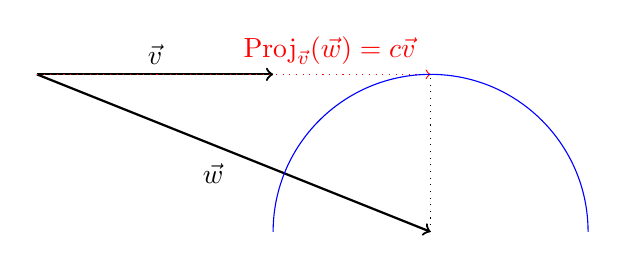
\begin{tikzpicture}
			\node (x) at (0,0){};
			\node (y) at (5,0){};
			\node (z) at (5,-2){};
			\draw[->,thick]
			(0,0) -- (3,0) node [midway, above] {$\vec{v}$};
			\draw[->,thick]
			(0,0) -- (5,-2) node[midway, below left]{$\vec{w}$};
			\draw[dotted]
			(5,-2) -- (5,0);
			\draw[->,red,dotted] 
			(0,0)--(5,0) node[midway, above right]{$\textrm{Proj}_{\vec{v}}(\vec{w}) = c\vec{v}$};
			
			\draw [blue](7,-2)arc (0:180:2);
		
		\end{tikzpicture}
	\end{subfigure}
\end{figure}
	
	
	

We also see from this geometric construction that 1) the projection $c\vec{v}$ is unique thus well defined, 2) $c|\vec{v}|=|\vec{w}|\cos \theta$

\proposition{
The projection is unique and is given by \[
	\textrm{Proj}_{\vec{v}}(\vec{w}) = \frac{\cos \theta |\vec{w}|}{|\vec{v}|} = \frac{\vec{v}\cdot\vec{w}}{|\vec{v}|^2} = \left(\frac{\vec{v}\cdot\vec{w}}{\vec{v}\cdot\vec{v}}\right)\vec{v}.
\]

}
This is the first time we show that something is unique. The standard argument goes as follows: Suppose another object $a'$ satisfies all the properties you want for $a$. Then you can show $a=a'$, meaning every object that satisfies the properties is $a$, or equivalently, $a$ is unique. 

So what happens if we pick two points $P$, $P'$ on $\vec{v}$ such that both make a right angle when connected to $\vec{w}$? We would have constructed a triangle $\triangle PP'\vec{w}$ with two right angles!
\begin{proof}
	Let $c, c'\in\reals$ such that $\vec{p}_1=c\vec{v}$ and $\vec{p}_2=c'\vec{v}$ are both satisfy the definition of $\textrm{Proj}_{\vec{v}}({\vec{w}})$. We want to show that $c=c'$, so we consider $\vec{u}=(c-c')\vec{v}$, the line between the two projections.\\
	By corollary \ref{cor:dotproduct}, we have two equations \begin{align*}
	|\vec{w}-\vec{p}_1|^2&=|\vec{w}-\vec{p}_2|^2+|\vec{u}|^2 \\	
	|\vec{w}-\vec{p}_2|^2&=|\vec{w}-\vec{p}_1|^2+|\vec{u}|^2 
	\end{align*}
	We can solve for $|\vec{u}|=0$, and by positive definiteness, $\vec{u}=\vec{0}$ and $c-c' = |\vec{u}|/|\vec{v}| =0$.\\
	To show our formula for projection works, we can just compute that \[
	\vec{v} \cdot \left(\vec{w}-\left(\frac{\vec{v}\cdot{\vec{w}}}{\vec{v}\cdot\vec{v}}\right)\vec{v}\right)=\vec{v}\cdot\vec{w} -\left(\frac{\vec{v}\cdot\vec{w}}{\vec{v}\cdot\vec{v}}\right)(\vec{v}\cdot\vec{v})=0.
	\]
\end{proof}
\exercises
\begin{exerciselist}
	\item Determine if the following pairs of vectors are orthogonal: \begin{enumerate}[label=(\alph*)]
		\item $3\vec{e}_1+4\vec{e}_2$, $-4\vec{e}_1+3\vec{e}_2$
		\item $(4,-1,2)$, $(3,0,-6)$
		\item $3\vec{i}-2\vec{j}$, $-2\vec{i}-4\vec{k}$
		\item $\vec{e}_1 + 3\vec{e}_3 + 5\vec{e}_5+ ...+(2k-1)\vec{e}_{2k-1}$, $2\vec{e}_2+4\vec{e}_4+...+(2k)\vec{e}_{2k}$
	\end{enumerate}
	\item Refer to the plane in Example \ref{ex:1.26}. Show that $\textrm{Proj}_{-3\vec{i}+2\vec{j}+6\vec{k}}(\vec{v})$ is the same for any vector $\vec{v}$ such that $\vec{v}\cdot(-3\vec{i}+2\vec{j}+6\vec{k}) =49$, and compute this projection.
	\item \textit{(Geometry of a methane molecule)} Place four points $P(0,0,0)$, $Q(1,1,0)$, $R(1,0,1)$, $S(0,1,1)$ in $\reals^3$. \begin{enumerate}[label=(\alph*)]
		\item Compute the distance between any two points of $PQRS$ and show that all $6$ pairs are the same. This means that $PQRS$ forms a regular tetrahedron.
		\item  Verify that the geometric center of the tetrahedron $O(1/2, 1/2, 1/2)$ is equidistant to all of the vertices of the tetrahedron.
		\item Compute the angle between two edges of the tetrahedron, rounded to $2$ decimal places. By symmetry, you only have to compute one angle.
		\item Compute the angle $\angle POQ$, rounded to $2$ decimal places. Does this angle remind you of something from Chemistry?
	\end{enumerate}
\end{exerciselist}
\section{Cross Product}
\definition{Cross Product}{
Let $\vec{v},\vec{w}\in\reals^3$, we define the \textbf{cross product} of $\vec{v}$ and $\vec{w}$ to be \[
	\vec{v}\times\vec{w}\defeq \begin{bmatrix}
		v_2w_3-v_3w_2\\
		v_3w_1 - v_1w_3\\
		v_1w_2 - v_2w_1\\
	\end{bmatrix}.
\]
}
\begin{remark}
	Later on, we will introduce determinants of a matrix. The cross product can be understood as the determinant of the `matrix'\[
	\begin{bmatrix}
		\vec{i} & v_1 & w_1 \\
		\vec{j} & v_2 & w_2 \\
		\vec{k} & v_3 & w_3
	\end{bmatrix}.
	\]
\end{remark}
This definition seems a bit unmotivating, so let us work through some examples.
\example{
	Compute the $9$ cross products for each pair of the standard basis vectors in $\reals^3$.
}
With some (heavy) computation, we find
\begin{align*}
	\vec{i}\times\vec{i}&=\vec{0} \quad& \vec{i}\times\vec{j}&=\vec{k} \quad& \vec{i}\times\vec{k}&=-\vec{j} \\
	\vec{j}\times\vec{i}&=-\vec{k} \quad& \vec{j}\times\vec{j}&=\vec{0} \quad& \vec{j}\times\vec{k}&=\vec{i}\\
	\vec{k}\times\vec{i}&=\vec{j} \quad& \vec{k}\times\vec{j}&=-\vec{i} \quad& \vec{k}\times\vec{k}&=\vec{0}
\end{align*}
Importantly, the cross product is \textbf{antisymmetric}, meaning $\vec{v}\times\vec{w}=-\vec{w}\times\vec{v}$. You can see special cases with the standard basis from above and confirm the general case in an exercise.
\example{
	Compute $\vec{v} \cdot (\vec{v}\times\vec{w})$ and $\vec{w}\cdot (\vec{v}\times\vec{w})$.
}
Again with some heavy computation,
\begin{align*}
	\vec{v} \cdot (\vec{v}\times\vec{w}) &= \begin{bmatrix}
		v_1 \\v_2\\v_3
	\end{bmatrix}\cdot\begin{bmatrix}
	v_2w_3-v_3w_2\\
	v_3w_1 - v_1w_3\\
	v_1w_2 - v_2w_1\\
	\end{bmatrix} \\
	&= \color{red}v_1v_2w_3\color{black}-\color{black}v_1v_3w_2\color{black}+\color{blue}v_2v_3w_1\color{black}-\color{red}v_2v_1w_3\color{black}+\color{black}v_3v_1w_2\color{black}-\color{blue}v_3v_2w_1\\
	&=0,\\
	\vec{w} \cdot (\vec{v}\times\vec{w}) &= \begin{bmatrix}
		w_1 \\w_2\\w_3
	\end{bmatrix}\cdot\begin{bmatrix}
		v_2w_3-v_3w_2\\
		v_3w_1 - v_1w_3\\
		v_1w_2 - v_2w_1\\
	\end{bmatrix} \\
	&= \color{red}w_1v_2w_3\color{black}-\color{black}w_1v_3w_2\color{black}+\color{black}w_2v_3w_1\color{black}-\color{blue}w_2v_1w_3\color{black}+\color{blue}w_3v_1w_2\color{black}-\color{red}w_3v_2w_1\\
	&=0.\\
\end{align*}
Which means $\vec{v}\times\vec{w}$ is orthogonal to $\vec{v}$ and $\vec{w}$!

\example{
	Compute $|\vec{v}\times\vec{w}|^2 + (\vec{v}\cdot\vec{w})^2$.
}
We have
\begin{align*}
|\vec{v}\times\vec{w}|^2 + (\vec{v}\cdot\vec{w})^2 =&
(v_2w_3-v_3w_2)^2 +(v_3w_1 - v_1w_3)^2 + (v_1w_2 - v_2w_1)^2 
\\ &+ 
(v_1w_1 + v_2w_2 + v_3w_3)^2\\
=& (v_1w_1)^2+(v_1w_2)^2+(v_1w_3)^2\\&+(v_2w_1)^2+(v_2w_2)^2+(v_2w_3)^2\\&+(v_3w_1)^2+(v_3w_2)^2+(v_3w_3)^2\\
=&(v_1^2 + v_2^2+v_3^2)(w_1^2+w_2^2+w_3^3)\\
=&|\vec{v}|^2|\vec{w}|^2.
\end{align*}
Now we substitute $\vec{v}\cdot\vec{w}=|\vec{v}||\vec{w}|\cos\theta$, we get \[
	|\vec{v}\times\vec{w}|=|\vec{v}||\vec{w}|\sqrt{1-\cos^2\theta} = |\vec{v}||\vec{w}|\sin\theta.
\]
Where we know $\sin \theta \geq 0$ as $\theta$ is between $0$ and $\pi$.

The value $|\vec{v}||\vec{w}|\sin\theta$ has a nice geometric meaning. It is the area spanned by the vectors $\vec{v}$ and $\vec{w}$.\ \\
\usetikzlibrary{angles} 
\begin{figure}[h]%{r}{0.4\textwidth}
	\centering
\begin{tikzpicture}
	\node (X)[draw=none] at (0,0) {};
	\node (Y)[draw=none] at (5,0) {};
	\node (XT)[draw=none] at (-2,-2) {};
	\node (YT)[draw=none] at (3,-2) {};
	
	\draw[->,thick] 
	(0,0)--(5,0)
	node (a)[midway, above left] {$\vec{w}$};
	
	\draw[->,thick] 
	(0,0)--(-2,-2)
	node[midway, above left] {$\vec{v}$};
	
	\draw[->,dotted] 
	(5,0)--(3,-2)
	node[midway, above left] {$\vec{v}$};
	
	
	\draw[->,dotted] 
	(-2,-2)--(3,-2)
	node[midway, below left] {$\vec{w}$};
	\pic [pic text=$\theta$,draw,angle eccentricity=1.5] {angle = XT--X--Y};
	\draw[dotted]
	(0,0)--(-2,0) node (O) {}--(-2,-2)
	node [midway, left]{$|\vec{v}|\sin\theta$};
	\pic [draw, angle eccentricity=0.5]{right angle=XT--O--X};
\end{tikzpicture}
\caption {The area of a parallelogram formed by these vectors is the magnitude of the vector $\vec{v}\times|\vec{w}|$}
\end{figure} \ \\
\proposition{
	The direction of $\vec{v}\times\vec{w}$ is determined by the \textbf{right-hand rule} as follows:
	\begin{quotation}
		Using the right hand, align the index finger with the direction $\vec{v}$, and the middle finger with the direction of $\vec{w}$. Extend the thumb so that it is perpendicular to both the index finger and the middle finger. The thumb is pointing in the direction of $\vec{v}\times \vec{w}$.
	\end{quotation}
}
This is a byproduct of the convention we use. In $\reals^3$ we use what is known as a right-handed coordinate system - the vectors $\vec{i}$, $\vec{j}$, and $\vec{k}$ align with the first three fingers of the right hand respectively. If we used a left-handed coordinate system, the rule would be left-handed instead. 
\begin{figure}[h]
	\centering
	\begin{subfigure}[l]{0.4\textwidth}
		\centering
		\begin{tikzpicture}
			
			\draw[->](0,0,0) -- (xyz cylindrical cs:radius=3);
			\node at (3.5,0,0){$x_2$};
			\draw[->] (0,0,0) -- (xyz cylindrical cs:radius=3,angle=90);
			\node at (0,3.5,0){$x_3$};
			\draw[->] (0,0,0) -- (xyz cylindrical cs:z=3);
			\node at (0,0,3.5){$x_1$};
		\end{tikzpicture}
		\caption {Right handed coordinate system}
	\end{subfigure}
	\begin{subfigure}[r]{0.4\textwidth}
		\centering
			\begin{tikzpicture}
			\draw[->](0,0,0) -- (xyz cylindrical cs:radius=3, angle=180);
			\node at (-3.5,0,0){$x_2$};
			\draw[->] (0,0,0) -- (xyz cylindrical cs:radius=3,angle=90);
			\node at (0,3.5,0){$x_3$};
			\draw[->] (0,0,0) -- (xyz cylindrical cs:z=3);
			\node at (0,0,3.5){$x_1$};
		\end{tikzpicture}
		\caption {Left handed coordinate system}
	\end{subfigure}
\end{figure}
We now have a few properties about the cross product from our computation, the first you will verify on your own:
\proposition{
	Let $\vec{v},\vec{w},\vec{u}\in\reals^n$, then 
	\begin{itemize}
		\item \textit{(distributivity)} $\vec{v}\times(\vec{u}+\vec{w})=\vec{v}\times\vec{u}+\vec{v}\times\vec{w}$ and $(\vec{v}+\vec{u})\times\vec{w}=\vec{v}\times\vec{w}+\vec{v}\times\vec{u}$.
		\item \textit{(anti-symmetry)} $\vec{v}\times\vec{w}=-\vec{w}\times\vec{v}$.
		\item $\vec{v}\times\vec{w}$ is orthogonal (perpendicular in 3D space) to $\vec{v}$ and $\vec{w}$.
		
		\item The magnitude $|\vec{v}\times\vec{w}|$ is given by $|\vec{v}||\vec{w}|\sin\theta$, with $\theta$ being the angle between $\vec{v}$ and $\vec{w}$, so \begin{enumerate}[label=(\roman*)]
			\item The magnitude $|\vec{v}\times\vec{w}|$ also corresponds to the area of the parallelogram formed by $\vec{v}$ and $\vec{w}$.
			\item If $\vec{v}$ and $\vec{w}$ are parallel or antiparallel, $\vec{v}\times\vec{w}=\vec{0}$.
		\end{enumerate}		
	\end{itemize}
}
\begin{remark}
	Using distributivity of the cross product, you only need to memorize the cross product of the basis vectors, and write $\vec{v}\times\vec{w}=\sum_{i=1}^{3}\sum_{j=1}^3v_iw_i (\vec{e}_i\times\vec{e}_j)$.
\end{remark}
\subsection{Triple products}
\example{
	Find the volume of the parallelepiped formed from $\vec{v}=\begin{bmatrix}
	0\\1\\1
	\end{bmatrix}$, $\vec{w}=\begin{bmatrix}
	1\\1\\0
	\end{bmatrix}$, $\vec{u}=\begin{bmatrix}
	1\\0\\1
	\end{bmatrix}$.
}

%\usetikzlibrary{perspective}

The parallelepiped is a generalization of a parallelogram to higher dimensions. Using combinations of $\vec{v},\vec{w},\vec{u}$, you can make the frame of a 3d solid. As in the figure on the left, edges of the same color correspond to the same vector (and thus parallel). The volume of this solid is still $base \times height$, where the base is a 2D parallelogram formed by two vectors and the height is determined by third vector. We make an arbitrary decision and set the base to be $\vec{v}$ and $\vec{w}$. (setting any two vectors would give the same result in the end!) The area of this base is given by the cross product
\[
	\vec{A}=\vec{v}\times\vec{w} = \begin{bmatrix}
		-1\\1\\-1
	\end{bmatrix}.
\]\ \\

Now we can determine the height of the paralellepiped from $\vec{u}$. We want to isolate the component of $\vec{u}$ that is orthogonal to the base. Equivalently, we want to find the component of $\vec{u}$ that is pointing in the direction of $\vec{A}$, a vector that is orthogonal to both $\vec{v}$ and $\vec{w}$!\ \\
\begin{figure}[h]%{r}{\textwidth}
	\centering
	\begin{subfigure}{0.4\textwidth}
		\centering
		\begin{tikzpicture}
			[z={(10:10mm)},x={(-45:5mm)}]
			
			\draw[->](0,0,0) -- (xyz cylindrical cs:radius=3);
			\node at (3.5,0,0){$x_1$};
			\draw[->] (0,0,0) -- (xyz cylindrical cs:radius=3,angle=90);
			\node at (0,3.5,0){$x_2$};
			\draw[->] (0,0,0) -- (xyz cylindrical cs:z=3);
			\node at (0,0,3.5){$x_3$};
			\draw[->,color=red] 
			(0,0,0)--(0,1,1)
			node[midway, below] {\color{red}$\vec{v}$};
			\draw[->,color=blue] 
			(0,0,0)--(1,0,1)
			node[midway,below]{\color{blue}$\vec{u}$};
			\draw[->,color=green] 
			(0,0,0)--(1,1,0)
			node[midway, left]{\color{green}$\vec{w}$};
			
			\draw[->,color=red] 
			(1,0,1)--(1,1,2);
			
			\draw[->,color=green] 
			(1,1,2)--(2,2,2);
			\draw[->,color=red] 
			(1,1,0)--(1,2,1);
			\draw[->,color=green] 
			(1,0,1)--(2,1,1);
			\draw[->,color=red] (2,1,1)--(2,2,2);
			\draw[->,color=green] 
			(0,1,1)--(1,2,1);
			
			\draw[->,color=blue] 
			(1,1,0)--(2,1,1);
			
			\draw[->,color=blue] 
			(1,2,1)--(2,2,2);
			\draw[->,color=blue]
			(0,1,1)--(1,1,2);
		\end{tikzpicture}
		\caption{The parallelepiped, draw in an optical illusion fashion.}
	\end{subfigure}
	\begin{subfigure}{0.4\textwidth}
		\centering
		\begin{tikzpicture}
			[z={(10:10mm)},x={(-45:5mm)}]
			
			\draw[->](0,0,0) -- (xyz cylindrical cs:radius=3);
			\node at (3.5,0,0){$x_1$};
			\draw[->] (0,0,0) -- (xyz cylindrical cs:radius=3,angle=90);
			\node at (0,3.5,0){$x_2$};
			\draw[->] (0,0,0) -- (xyz cylindrical cs:z=3);
			\node at (0,0,3.5){$x_3$};
			\draw[->,color=red] 
			(0,0,0)--(0,1,1)
			node[midway, below] {\color{red}$\vec{v}$};
			\draw[->,color=blue] 
			(0,0,0)--(1,0,1)
			node[midway,below]{\color{blue}$\vec{u}$};
			\draw[->,color=green] 
			(0,0,0)--(1,1,0)
			node[midway, left]{\color{green}$\vec{w}$};
			\draw[->,dotted,thick]
			(0,0,0)--(-1,1,-1)
			node[midway,left]{$\vec{A}$};
			\draw[->,color=red] 
			(1,1,0)--(1,2,1);
			\draw[->,color=green] 
			(0,1,1)--(1,2,1);
			
		\end{tikzpicture}
		\caption{We want to get the projection of $\vec{u}$ on $\vec{A}$.}
	\end{subfigure}
\end{figure}\ \\
The volume is thus \[
	|\textrm{Proj}_{\vec{A}}(\vec{u})||\vec{v}|=\left|\frac{\vec{u}\cdot\vec{A}}{|\vec{A}|^2}\right|\times |\vec{A}| \times|\vec{A}| = |\vec{u}\cdot\vec{A}| = 2.
\]\ \\

\proposition{
The volume of the parallelpiped formed from $\vec{v},\vec{w},\vec{u}$ is \[
|(\vec{v}\times\vec{w})\cdot{\vec{u}}|
\]
}\ \\

\begin{remark}
	This is also the expression of the (absolute value of) determinant of \[
	\begin{bmatrix}
		\vec{v}&\vec{w}&\vec{u}
	\end{bmatrix}
	\]
	where $\vec{v},\vec{w},\vec{u}$ are written as column vectors.
	Using properties of the determinant (later chapters), you can show cycling the three vectors does not change the volume. (i.e. you can calculate using what order of the three vectors you want)
\end{remark}
	
\begin{remark}
	You may notice that the expression $(\vec{v}\times\vec{w})\cdot{\vec{u}}$ can take on negative volumes. In this case, the three vectors (taken in order) do not follow the right-hand rule. For instance, in the last example, $\vec{u}$ points in the `opposite' direction as $\vec{A}$.
\end{remark}
\exercises
\begin{exerciselist}
	\item Find $\vec{v}\times\vec{w}$ for the following: \begin{enumerate}[label=(\alph*)]
		\item $\vec{v}=(4,-2,0)$, $\vec{w}=(2,1,-1)$
		\item $\vec{v}=(3,3,3)$, $\vec{w}=(4,-3,2)$
		\item $\vec{v}=2\vec{i}+3\vec{j}+4\vec{k}$, $\vec{w}=\vec{i}-3\vec{j}+4\vec{k}$
	\end{enumerate}
	\item Find the areas for the following shapes:\begin{enumerate}[label=(\alph*)]
		\item The parallelogram with vertices $P(0,0,0), Q(1,1,0),R(1,2,1),S(0,1,1)$.
		\item The triangle with vertices $A(1,9,3),B(-2,3,0),C(3,-5,3)$.
	\end{enumerate}
	\item Find the volume of the parallelepiped formed from the vectors $\vec{v}=(1,1,0),\vec{w}(0,2,-2),\vec{u}=(1,0,3)$.
	\item A triangular kite has vertices $P(0,0,10),Q(2,1,10),S(0,3,12)$ and is displaced by the wind at a velocity of $(20\vec{i}+6\vec{j}+4\vec{k})/s$\begin{enumerate}[label=(\alph*)]
		\item Find the area of the kite.
		\item After 1/2 seconds, find the volume of the space swept by the kite. (leave the answers in $[units]^3$)
	\end{enumerate}
\end{exerciselist}

\section{Applications - Geometry of lines and planes}
\definition{Relations between lines}{
For two (infinitely extending) lines in $\reals^n$ parametrized in $s$ and $t$ respectively as $l_1=P + t\vec{v}$, $l_2=Q+s\vec{w}$, we say the lines are \begin{itemize}
	\item \textbf{Parallel}, if the $\vec{v}$ and $\vec{w}$ are parallel or antiparallel.
	\item \textbf{Intersecting}, if $l_1$ and $l_2$ exactly one point on both $l_1$ and $l_2$.
	\item \textbf{Skew}, if $l_1$ and $l_2$ are not parallel/antiparallel or intersecting.
\end{itemize}
}
\begin{remark}
	Lines do not have direction, so there usually is no need to distinguish between parallel and antiparallel lines. One may extend the definition of antiparallel to lines from $\vec{v}$ and $\vec{w}$.
\end{remark}
\proposition{
Determination of parallel lines are independent of parametrization. Concretely, 
\begin{quotation}
Let $P_1+t_1\vec{v}_1$ and $P_2+t_2\vec{v}_2$ be two parametrizations of $l_1$, $Q_1+s_1\vec{w}_1$, $Q_2+s_2\vec{w}_2$ be two parametrizations of $l_2$. If $\vec{v}_1 =c_1\vec{w}_1$ for some $c_1\in\reals$, then $\vec{v}_2=c_2\vec{w}_2$ for some (possibly different )$c_2\in\reals$.
\end{quotation}
}
The proof is not very enlightening. However, the result of this guarantees that our definition of parallel lines is precise.
\begin{proof}
	The idea is to show that $\vec{v}_1$ is a scalar multiple of $\vec{v}_2$, and by the same logic $\vec{w}_1$ is a scalar multiple of $\vec{w}_2$. Since all vectors are non-zero in the parametrization, we will get the result of $\vec{v}_2$ a scalar multiple of $\vec{w}_2$. 
	
	To show $\vec{v}_1=k\vec{v}_2$ for some $k$, we can pick two distinct points $A,B$ on $l_1$. From the parametriation we can get $\alpha_1,\alpha_2,\beta_1,\beta_2\in\reals$ such that $P_1+\alpha_1\vec{v}_1=A=P_2+\alpha_2\vec{v}_2$ and $P_1+\beta_1\vec{v}_1=B=P_2+\beta_2\vec{v}_2$. Therefore we get the vector \begin{align*}
		\overrightarrow{AB}&=(\beta_1-\alpha_1)\vec{v}_1,\\
		\overrightarrow{AB}&=(\beta_2-\alpha_2)\vec{v}_2.
	\end{align*}
	As we picked distinct points $A$ and $B$, we can conclude $\overrightarrow{AB}\neq\vec{0}$ and thus $\beta_1-\alpha_1\neq0,\beta_2-\alpha_2\neq0$, so that \[
		\vec{v}_1= \frac{\beta_2-\alpha_2}{\beta_1-\alpha_1}\vec{v}_2.
	\]
\end{proof}
\example{
Determine whether the lines parametrized by $l_1(t)=(1,2,1)+t(1,3,-2)$ and $l_2(t)=(3,1,0)+t(-2,-6,4)$ are parallel, intersecting, or skew. Confirm that $l_1$ and $l_2$ describe two different lines. 
}
We notice that $-2\times(1,3,-2)=(-2,-6,4)$, so these lines are parallel. To confirm that these two lines are not the same, we notice that $(1,2,1)$ is a point on $l_1$, but if we attempt to solve\[
(1,2,1)=l_2(t)=(3,1,0)+t(-2,-6,-4) \implies (-2,1,1)=t(-2,-6,-4) 
\]
which no $t$ can solve! Specifically, the first coordinate forces $t=1$ and the second coordinate forces $t=-6$. 
\example{
Determine whether the lines parametrized by $l_1(t)=(1,2,1)+t(1,3,-2)$ and $l_2(t)=(0,3,9)+t(0,2,3)$ are parallel, intersecting, or skew.
}
$(1,3,2)$ is not a multiple of $(0,2,3)$, so the lines are not parallel. We might be tempted to solve for $l_1(t)=l_2(t)$ to check for intersection, but this misses a lot of cases! We need to compare all the points of $l_1$ with all the points of $l_2$, so we need two independent variables to describe where we are on each of the lines. That is, we solve for $s,t$ in $l_1(t)=l_2(s)$,
\begin{align*}
	(1,2,1)+t(1,3,-2) &=(0,3,9)+s(0,2,3)\\
	\implies (t+1,3t+2,-2t+1) &= (0,2s+3,3s+9)\\
	\implies t=-1 \textrm{ and } &3t+2=2s+3 \textrm{ and } -2t+1=3s+9
\end{align*}
$t=-1, s=-2$ solves this system of equations. We can plug in $t$ and $s$ in our original parametrization to find $(0,1,3)$ is indeed a point on both $l_1$ and $l_2$. We would have missed this if we set $l_1(t)=l_2(t)$! 
\example{
	Determine whether the lines parametrized by $l_1(t)=(1,2,1)+t(1,3,-2)$ and $l_2(t)=(0,3,8)+t(0,2,3)$ are parallel, intersecting, or skew.
}
We repeat the same process as above to see that the lines are not parallel and solve for 
\begin{align*}
	(1,2,1)+t(1,3,-2) &=(0,3,8)+s(0,2,3)\\
	\implies (t+1,3t+2,-2t+1) &= (0,2s+3,3s+8)\\
	\implies t=-1 \textrm{ and }& 3t+2=2s+3 \textrm{ and } -2t+1=3s+8
\end{align*}
This time, we do not have a solution - the first two equations forces $t=-1, s=-2$, and this does not solve the third. We therefore do not have a point of intersection, and the lines are skew.
\example{
	Determine if $P(5,6,9), Q(7,9,15), R(13,18,33)$ are \textbf{colinear} i.e. if they lie on the same line. 
}
With the machinery we have built up, there are multiple ways to check if $P,Q,R$ form a straight line. Here are a few ideas:\begin{enumerate}
	\item Check that $\overrightarrow{PQ}$ is parallel/antiparallel to $\overrightarrow{PR}$. Because the lines defined by $\overline{PQ}$ and $\overline{PR}$ are parallel and share a same point $P$, they are the same line.
	\item Use the dot product to calculate the angle $\angle PQR=\pi$.
	\item Use the cross product to calculate that $\overrightarrow{PQ}\times\overrightarrow{PR}=\vec{0}$. This means the triangle with vertices $P,Q,R$ has no area and thus is a degenerate triangle.

\end{enumerate}
\definition{Characterization of Planes}{
	In euclidean geometry, planes can be characterized by any of the following ways: \begin{itemize}
		\item For \textbf{any three non-colinear points} $P_1,P_2,P_3$, there is a unique plane passing through $P_1,P_2,P_3$.
		\item For \textbf{any pair of intersecting lines}, there is a unique plane that contains both.
		\item For \textbf{a line $l$ and a point $P$}, there is a unique plane that contains $P$ and is perpendicular to $l$.
		\item For \textbf{a line $l$ and a point $P$ not on $l$}, there is a unique plane that contains both $l$ and $P$.
	\end{itemize}
}
\begin{remark}
	The third characterization is the hardest to visualize at first, but is also the easiest to describe with the analytical tools we have built towards. We can refer to Example \ref{ex:1.26}. The plane sketched is the unique plane that contains $(-3,2,6)$, such that each vector in the plane is orthogonal to $(-3,2,6)$, so the line parametrized by $l(t)=t(-3,2,6)$ is perpendicular to the plane at the point of intersection $(-3,2,6)$.
\end{remark}

\example[1.44]{
	In $\reals^3$, determine the equation of the plane that contains $P_0(x_0,y_0,z_0)$ and is perpendicular to the line parametrized by $l(t)=Q_0+t\vec{N}$, $\vec{N}=(a,b,c)$.
}
First we can exploit \textbf{translation invariance} of $\reals^3$ and move the line to $\tilde{l}=P_0 + t\vec{N}$. Because $l$ and $\tilde{l}$ are parallel, any line perpendicular to $l$ will also be perpendicular to $\tilde{l}$.\\
Then by the characterization of a plane, any $P$ on the plane satisfies the orthogonality relation $\overrightarrow{PP_0}\cdot\vec{N}=0$. Expanding this, we get the equation \[
a(x-x_0)+b(y-y_0)+c(z-z_0)=0 \implies ax+by+cz=ax_0+by_0+cz_0.
\]
\definition{Normal form of a plane}{
Let $a,b,c,d\in\reals$, with at least one of $a,b,c\neq0$. The equation of a plane in $\real^3$ written as \[
ax+by+cz=d
\]
is called a \textbf{normal form} of the equation of a plane.
}
\begin{remark}
	As all planes can be characterized this method, all equations of planes can be put in normal form.
\end{remark}
\begin{remark}
	The normal form of a plane is not unique. Pick your favorite non-zero number $\alpha$, the equation $\alpha ax+\alpha by+\alpha c_z=\alpha d$ describes the same plane.
\end{remark}
\theorem[normalvectorofplane]{Normal vectors of planes}{
When written in normal form, the plane is perpendicular to the vector $\vec{N}=(a,b,c)$. We call this vector $\vec{N}$ the \textbf{normal vector}.
}
We thus have a definition for two planes to be parallel.
\definition{Parallel planes}{
Two planes are \textbf{parallel} if the normal vectors are parallel.
}
A problem in the exercise will guide you through the proof of Theorem \ref{thm:normalvectorofplane}. The intuition behind the proof is the reverse direction of the equation $\overrightarrow{PP_0}\cdot\vec{N}=0$ we derived from the last example.\\
We will now apply this theorem in a few examples.
\example{
Find the equation of the plane that passes through the points $P(1,0,0),Q(0,1,0),R(0,0,1)$.
}
\textbf{Method 1:} One sees that (by coincidence) the sum of coordinates of each point are equal to $1$, so immediately writes down $x+y+z=1$. Despite being the fastest method, this is somewhat inconsistent.\\


\textbf{Method 2:} We set $ax+by+cz=d$ to be the equation, and plug in values for $P,Q,R$, giving the system of equations\begin{align*}
	a+0b+0c&=d \\ 0a+b+0c&=d \\ 0a+0b+c&=d 
\end{align*}
This is an \textbf{underdetermined system}, meaning there are fewer equations than unknowns. The best we can say is that $a=b=c=d$. However, setting $a=b=c=d=k$ works for all $k\neq 0$, further confirming that the normal form is not unique. This method is reasonably fast when the system of equations are simple. When there are more non-zero coefficients, solving the system takes more time.\\

\textbf{Method 3:} We can compute the direction of the normal vector $\vec{N}$ of this plane. By the characterization of planes, $\vec{N}$ is orthogonal to $\overrightarrow{PQ}$ and $\overrightarrow{PR}$, two vectors in the plane. We can thus write $\vec{N}$ as a multiple of the cross product \[
	\overrightarrow{PQ} \times \overrightarrow{PR} = \begin{bmatrix}
		-1\\1\\0
	\end{bmatrix} \times \begin{bmatrix}
	-1\\0\\1
	\end{bmatrix} = \begin{bmatrix}
	1\\1\\1
	\end{bmatrix}
\]. Using this normal vector (or any multiple of it) and applying the theorem, we get $x+y+z=d$, and substituting $P$ into the equation will give $x+y+z=1$. This method is more general and consistent, as the number of operations in a cross product is constant.

\example{
On the plane given by $ax+by+cz=d$, find the point on the plane that is closest to the origin.
}
\begin{wrapfigure}{r}{0.35\textwidth}
	\centering
	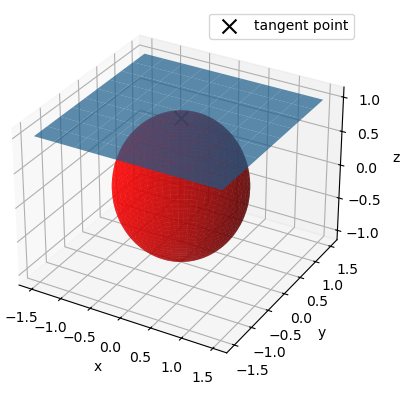
\includegraphics[width=0.3\textwidth]{coordinate_geometry/tangent.png}
	\caption{A toy example with the unit sphere of radius $1$ and the plane described by $z=1$.}
\end{wrapfigure}
Let $r$ be the distance, we draw a sphere centered at the origin with radius $r$. This sphere is thus tangent to the surface at one point, and the vector corresponding to this point will be perpendicular to the plane. By the theorem, we can denote the point $P(\alpha a, \alpha b, \alpha c)$, with $\alpha$ a constant to be determined. Substituting $P$ into the equation, \begin{align*}
	\alpha (a^2+b^2+c^2) = d \implies \alpha = \frac{d}{a^2+b^2+c^2}
\end{align*}
The closest distance from the origin is \[
|(\alpha a, \alpha b, \alpha c)| = |\alpha| \sqrt{a^2+b^2+c^2} = \left| \frac{d}{\sqrt{a^2+b^2+c^2}}\right| 
\]
at the point \[
\left(\frac{da}{\sqrt(a^2+b^2+c^2)},\frac{db}{\sqrt(a^2+b^2+c^2)},\frac{dc}{\sqrt(a^2+b^2+c^2)}\right)
\]\ \\
\subsection{Intersection of planes}
\example{
Find the intersection of the planes given by \begin{align*}
	6x+2y-z&=2\\
	\textrm{and } x-2y+3z&=5.
\end{align*}
}
\textbf{Method 1:} The line lies on the first plane, so is perpendicular to its normal vector $(6,-2,-1)$. The line also lies on the second plane, so is perpendicular to its normal vector $(1,-2,3)$. Using the cross product, the line should point in the direction of \[
\begin{bmatrix}
	6\\2\\-1
\end{bmatrix} \times\begin{bmatrix}
1\\-2\\3
\end{bmatrix}=\begin{bmatrix}
4\\-19 \\ -14
\end{bmatrix}
\]
Now we just need to find one point $P$ on the line of intersection, so that the parametric equation (in $t$) is $P+t(4,-19,-14)$.
We can impose an additional restriction that $x=0$ (or $y=0$ or $z=0$) and solve the simultaneous equations\begin{align*}
	2y-z&=2\\
	-2y+3z&=5.
\end{align*}
and get $(0,11/4,7/2)$ is a point on the intersection. The final parametric representation is $l(t)=(0,11/4,7/2)+t(4,-19,-14)$.

\textbf{Method 2:} We can solve the system of equations to find the line of intersection, and arrive at the set of symmetric equations. A similar method would be to solve for two points on the line of intersection, then get the parametric equation. This method will be introduced later\\
\exercises
\begin{exerciselist}
	\item Find parametric and symmetric equations for the line that \begin{enumerate}[label=(\alph*)]
		\item passes through $(0,0,0)$ and is parallel to $\vec{v}=3\vec{i}+4\vec{j}+5\vec{k}$
		\item passes through $(1,1)$ and is perpendicular to the line described by $y=3x+3$
		\item passes through $(0,1,2)$ and is perpendicular to plane with equation $3x+4y=2+z$
		\item passes through $(0,1,2)$ and is perpendicular to the yz-plane
		\item passes through $(1,3,0)$ and is parallel to the line with symmetric equations $x=y-1=(z-3)/2$
	\end{enumerate}
	\item Determine if these pair of lines are parallel, intersecting, or skew: \begin{enumerate}[label=(\alph*)]
		\item (As described by parametric equations) $l_1(t)=(1,-1,2)+t(2,1,1), l_2(t) = t(1,0,-1)$
		\item The line passing through $(3,1,3)$ and $(-2,-4,-5)$ and the line passing through $(1,3,5)$ and $(11,13,21)$.
	\end{enumerate}
	\item Determine if $P(3,1,2),Q(-1,0,2), R(11,3,2)$ are colinear.
	\item Find an equation for the plane \begin{enumerate}[label=(\alph*)]
		\item Containing $P(1,2,0)$ with normal vector $\vec{N}=2\vec{i}-\vec{j}+3\vec{k}$
		\item containing $P(2,4,5)$ with normal vector $\vec{N}=\vec{i}+3\vec{k}$
		\item containing $P(1,4,3)$ and perpendicular to the line given by the parametrization $r(t)=(1+t,2+4t,t)$
		\item containing the origin and parallel to the plane described by $3x+4y-6z=-1$
		\item containing the points $P(0,0,0),Q(1,-2,8),R(-2,-1,3)$
	\end{enumerate}
	\item Find the intersection of the planes with equations $2x+3y-z=1$ and $x-y-z=0$
	\item Find the angle between the normal vectors of the following planes: \begin{enumerate}[label=(\alph*)]
		\item the planes with equations $x+2y-z=2$ and $2x-y+3z=1$
		\item the plane with equation $2x+3y-6z=0$ and the plane containing the points $P(1,3,-2)$, $Q(5,1,3)$, $R(1,0,1)$
		\end{enumerate}
\end{exerciselist}

\section{End of Chapter Exercises}
\begin{exerciselist}
	\item Let $PQRS$ be a parallelogram. Show that $\overline{PR}$ and $\overline{QS}$ bisect each other i.e. intersect at their midpoints. 
	\item Complete the proof to Proposition \ref{1.22} - Show that the dot product is symmetric and linear. 
	\item Prove the \hyperref[thm:cauchyschwarz]{Cauchy-Schwarz inequality}. Here is a hint: Write $\vec{w} =  \textrm{Proj}_{\vec{v}}{\vec{w}} + (\vec{w}-\textrm{Proj}_{\vec{v}}{\vec{w}})$, and take the squared-magnitude on each side using the dot product.
	\item Prove or give a counterexample: The cross product is associative.
	\item Prove the following identity: $(\vec{a}\times\vec{b})\times\vec{c} = -(\vec{b}\cdot\vec{c})\vec{a}+(\vec{a}\cdot\vec{c})\vec{b}$.
	\item Show that the cross product satisfies the Jacobi identity: For any $\vec{a},\vec{b},\vec{c}\in \reals^3$, $(\vec{a}\times\vec{b})\times\vec{c} + (\vec{b}\times\vec{c})\times\vec{a} +(\vec{c}\times\vec{a})\times\vec{b} =\vec{0}$.
	\item On the plane given by $ax+by+cz=d$, show that the closest distance from $P(x_1,y_1,z_1)$ to the plane is given by $|ax_1+by_1+cz_1-d|/\sqrt{a^2+b^2+c^2}$. (Hint: Refer to Example \ref{ex:1.44})
	\item Define two lines in $\reals^3$ by the parametric equations \begin{align*}
		l_1(t) = \vec{r}_1 + t\vec{v}_1\\
		l_2(t)=\vec{r}_2+t\vec{v}_2
	\end{align*}
	We will derive a formula for the shortest distance between the two lines.
	\begin{enumerate}[label=(\alph*)]
		\item Consider the special case where the two lines are parallel. Construct two points $A$ and $B$ on $l_1$ and $l_2$ respectively. Find $B'$ Such that $\overrightarrow{AB'} = \textrm{Proj}_{\vec{v_1}}(\overrightarrow{AB})$. Argue that $B'$ is on the line $l_1$, and that the line $\overline{BB'}$ is perpendicular to $l_1$ and $l_2$. Conclude that the shortest distance between $l_1$ and $l_2$ is given by \[
			\sqrt{|\vec{r}_2-\vec{r}_1|^2 - \left(\frac{(\vec{r}_2-\vec{r_1})\cdot\vec{v}_1}{|\vec{v}_1|}\right)^2}
		\] 
		\item Now we can assume the lines are not parallel. Find a vector $\vec{N}$ that is perpendicular to both lines.
		\item (In your mind,) look in the direction of $\vec{N}$. $\vec{N}$ will now look like a dot. The lines will seem to overlap at points $A'$ and $B'$ respectively. Argue that $\overline{A'B'}$ is the shortest line from $l_1$ to $l_2$, and it is given by \[
			\overrightarrow{A'B'}=\textrm{Proj}_{\vec{N}}(\overrightarrow{AB})
		\], for any $A$ on $l_1$ and $B$ on $l_2$.
		\item Conclude that the shortest distance in this case is given by \[
			\left|\frac{(\vec{r}_2-\vec{r_1}) \cdot(\vec{v}_1\times\vec{v}_2)}{|\vec{v}_1\times\vec{v}_2|}\right|.
		\]
		\item Suppose $l_1$ and $l_2$ intersect at $P$. Verify that the formula evaluates to $0$, thus it gives a criterion to check if two lines intersect.
	\end{enumerate}
\end{exerciselist}

	%\chapter{Linear Algebra Basics}

\setcounter{exercisecounter}{0}

\setcounter{thmcounter}{0}
    The foundational abstraction of linear algebra is the vector space. A \textit{vector space} is essentially a collection of objects that it
makes sense to take linear combinations of. Two operations must be defined: addition and scalar multiplication. A well defined
vector space meets all of the vector space axioms, which will be listed shortly. Many consequences can be drawn from these axioms,
and we can build up linear algebra to solve any linear problem.

\begin{remark}
	One has to specify the field of scalars (\textit{field} just means number system) related to the vector space. In most cases
here, we will be talking about real vector spaces (the field of scalars is $\mathbb{R}$). However, vector spaces can be defined with
many other fields of scalars. Examples will follow the definition.
\end{remark}
\definition{Informal definition of a field}{
	A field $\mathbb{K}$ is a set that supports
	addition, subtraction, multiplication, division with the similar properties that you expect from the real numbers.
}
%\iffalse
\subsection*{Where is this going?}
In the previous chapter, we have seen vector manipulation in $\reals^n$. This chapter tries to generalize some observations we have about $\reals^n$ to other mathematical objects.
For now, we call these sets that have `$\reals^n$'-vector-like properties \textbf{vector spaces}. This notion is a bit abstract, and we usually default to $\reals^n$
to gain intuition about vector spaces and motivate new definitions and techniques. It just so happens that \textit{every finite dimensional real vector space is `almost the same' as $\reals^n$},
so many conclusions we get from $\reals^n$ naturally extend to other vector spaces.
%\fi

In the previous chapter, proposition \ref{prop:vectorspace} lists $8$ characteristics of $\reals^n$. Let us extract all these $8$
statements, and define a vector space to be a set that satisfies these properties.
\definition{Vector Space}{
	Let $\mathbb{K}$ be a field, and $V$ be a set closed under operations addition $+ : V\times V\to V$ and multiplication $\cdot : \mathbb{K} \times V \to V$. We call $V$ a \textbf{vector space}, or a \textbf{$\mathbb{K}$-vector space} to specify the field if the following axioms hold. \\
%	For all $\vec{u},\vec{v},\vec{w} \in V$, and $a,b \in \mathbb{K}$. 
	\begin{enumerate}
		\item \textit{(Associativity)} $x + (y + z) = (x + y) + z$  $\forall x, y, z \in V$.
		\item \textit{(Commutativity)} $x + y = y + x$  $\forall x, y \in V$.
		\item \textit{(Identity)} There exists some vector $0_V$ s.t. $x + 0_V = x$  $\forall x \in V$.
		\item \textit{(Inverse)} $\forall x \in V$,  $\exists y \in V$ s.t. $x + y = 0_v$.
		\item \textit{(Scalar multiplication)} $a \cdot (b \cdot x) = (a \cdot b) \cdot x$  $\forall a, b \in \mathbb{K}, x \in V$.
		\item \textit{(Scalar Identity)} $1 \cdot x = x$  $\forall x \in V$.
		\item \textit{(Distributivity 1)}  $a \cdot (x + y) = a \cdot x + a \cdot y$  $\forall a \in \mathbb{K}, x, y \in V$.
		\item \textit{(Distributivity 2)} $(a + b) \cdot x = a \cdot x + b \cdot x$  $\forall a, b \in \mathbb{K}, x \in V$.
	\end{enumerate}
} 
\example{
The following are examples of vector spaces.
\begin{itemize}
	\item $\reals^n$, with addition and multiplication as we have defined so far.
	\item $\{0_V\}$, the set containing just the zero vector, is a vector space over any field.
	\item The set of polynomials with degree $3$ or less. Addition and multiplication are defined as $(f+g)(x)=f(x)+g(x)$ and $cf(x)= c\times f(x)$.
	\item $\reals$ is a $\mathbb{Q}$-vector space, where $\mathbb{Q}$ is the set of all rationals (fractions).
\end{itemize}
%}
%\example{
	The following are non-examples of vector spaces.
	\begin{itemize}
		\item $\phi$, the empty set is not a vector space over any field as it does not have a zero vector.
		\item The set of polynomials with degree $3$ or more (using the addition and multiplication rules defined above).
		\item $\mathbb{Q}$ is not an $\mathbb{R}$-vector space. This is because $\pi(1)=\pi$ which is not in $\mathbb{Q}$.
	\end{itemize}
}
More frequently, we make new vector spaces from taking subsets of existing vector spaces. For instance, there might be a subset of $\reals^n$ that also satisfies all the axioms of being a vector space.

\definition{Subspace}{
	Let $V$ be a $\mathbb{K}$ vector space. We call $W\subseteq V$ a \textbf{subspace} of $V$ if $W$ forms a vector space using the inherited operations $+ : W\times W \to W$ and $\cdot : \mathbb{K}\times W \to W$. 
} 
\begin{remark}
	Because the inherited operations will automatically satisfy the axioms of a vector space, it suffices to show that (1) $W$ is nonempty and (2) $W$ is closed under vector addition and scalar multiplication to confirm that $W$ is a subspace.
\end{remark}
The condition $W$ is nonempty is required because the identity axiom requires a zero vector, which one obtains by multiplying $0$ to an arbitrary vector in the subset.
\example{
\begin{enumerate}
	\item In $\reals$-vector space $\reals^3$, the set of all vectors in the form of $k\vec{i}$ forms a subspace.
	\item Take $\reals$ as a $\mathbb{Q}$-vector space. $\mathbb{Q}\subset\mathbb{R}$ is a subspace. 
	\item Take $\reals$ as a $\mathbb{R}$-vector space. $\mathbb{Q}\subset\mathbb{R}$ is \textbf{not} a subspace because it is not closed under multiplication. 
\end{enumerate}
}
\proposition{
Let $W,U\subseteq V$ be subspaces. The intersection $W\cap U$ is a subspace of $V$.
}
\begin{proof}
	Both $W$ and $U$ contain $0_V$, so the intersection is non-empty. We also have for $v_1,v_2\in W\cap U$,\[
		v_1 + v_2 \in U, \quad v_1+v_2\in W,
	\] so addition is closed in $W\cap U$. Similarly, scalar multiplication closed under $W$ and $U$, so is closed in the intersection.
\end{proof}
\exercises
\begin{exerciselist}
	\item Determine if the following sets are real vector spaces:\begin{enumerate}[label=(\alph*)]
		\item The set of $(x,y,z)\in \reals^3$ that satisfy $2x+3y-z=0$. 
		\item The set of $(x,y,z)\in \reals^3$ that satisfy $2x+3y-z=4$.
		\item  The set of $(x,y,z)\in \reals^3$ that satisfy $x^2+y^2-z^2=0$.
		\item The set of real polynomials $f(x)=ax^3+bx^2+cx+d$ for all real constants $a,b,c,d$, such that $f^\prime (x)=0$.
		\item The set of continuous functions $f:\reals\to\reals$ such that $f(0)=1$.
	\end{enumerate}
	\item Give an example of a vector space that only has one subspace.
	\item Give a subspace of $\reals^4$ (that is not $\reals^4$) that contains the vector $(-1,3,0,7)$.
\end{exerciselist}


	%\section{Span, Linear Independence}
\subsection{Span}
Throughout this section, let $\mathbb{K}$ be a field. We constrain ourselves to work in $V$, a $\mathbb{K}$-vector space.
\definition{Span}{
	Let $k$ be some positive integer. Let  $\{v_1, v_2, ... , v_k\}\subseteq V$. The \textbf{span} of $\{v_1, v_2, ... , v_k\}$ is denoted as \[
	\textrm{span}(v_1,v_2,...,v_k)
	\]
	and is the \textit{smallest} subspace of $V$ containing $\{v_1, v_2, ... , v_k\}$.
	If $\textrm{span}(v_1,v_2,...,v_k) = V$, we say that $\{v_1,v_2,...,v_k\}$ is a spanning set of $V$, or $\{v_1,v_2,...,v_k\}$ spans $V$.
}
The \textit{smallest} here means that if another subspace $W$ contains $\{v_1,...,v_k\}$, $W$ cannot be a subset of $\textrm{span}(v_1,...,v_k)$. How do we know such a subspace exists? We can take the intersection of all the subspaces containing $\{v_1,...,v_k\}$ \[
\textrm{span}(v_1,...,v_k) = \bigcap_{W \textrm{ subspace containing } \{v_1,...,v_k\}} W
\]
which is a subspace containing $\{v_1,...,v_k\}$ and is a subset of all other subspaces containing $\{v_1,...,v_k\}$. We know $V\subseteq V$ is a subspace containing $\{v_1,...,v_k\}$, so the intersection is between at least one set and is thus well-defined.
\proposition{
     The span of $\{v_1, v_2,\ ... , v_k\}\subseteq V$ is 
    all linear combinations of the vectors in the set:
    \[\textrm{span}\{v_1, v_2,\ ... , v_k\} = \{c_1v_1 + c_2v_2 + ... + c_kv_k | c_1, c_2, ... c_k \in \mathbb{K}\}\]
}
\begin{proof}
	We first show $\textrm{span}\{v_1, v_2, ... , v_k\} \supseteq \{c_1v_1 + c_2v_2 + ... + c_kv_k | c_1, c_2, ... c_k \in \mathbb{K}\}$. That is, for every $W$ subset containing $v_1,...,v_k$, $W$ must also contain $c_1v_1+...+c_kv_k$. \\
	We now show $\textrm{span}\{v_1, v_2, ... , v_k\} \subseteq \{c_1v_1 + c_2v_2 + ... + c_kv_k | c_1, c_2, ... c_k \in \mathbb{K}\}$. The right side is a set that nonempty, is closed under addition and scalar multiplication, and contains $v_1= 1v_1+0v_2+...+0v_k$,...,$v_k=0v_1+...+0v_{k-1}+1v_k$. Therefore, it is one of the $W$ subspaces whose intersection is used to construct the span.
\end{proof}

% insert examples including what the span of one, two, etc. vectors is

It can be difficult to how to think about what the span of a set of vectors looks like, though it is also important to develop
an intuition for it as more complex techniques are developed. It is also important to consider what vectors span a given subspace.

\example{
	Sketch, in $\reals^3$, the following spans: span$(\{\vec{i}\})$, span$(\{\vec{i},\vec{j}\})$, span$(\{\vec{i},\vec{j},\vec{k}\})$.
}
\todo write something here\\
\subsection{Linear Independence}
Thinking geometrically in the previous example, the span of one vector is one-dimensional (a line), the span of two vectors is two-dimensional (a plane),
and the span of three vectors is three-dimensional (the whole 3D space). Specifically,
we can give a correspondence between the linear combination of $k$ vectors $\{c_1{v}_1,...,c_k{v}_k\}$and a point in $\reals^k$ as \[
	c_1{v}_1+c_2{v}_2+...+c_k{v}_k \sim \begin{bmatrix}
		c_1 \\ c_2\\ ...\\ c_k
	\end{bmatrix}
\]
Assuming this correspondence works, the geomtry of the span should resemble $\reals^k$.
Unfortunately, this is not always true, for instance, consider the following counterexample:
\example{
	Sketch, in $\reals^3$, $\textrm{span}(\vec{i},\vec{k},\vec{i}+2\vec{k})$.
}
\todo

What went wrong here is that the third vector $\vec{i}+2\vec{k}$ is already a linear combination of the first two, and so this vector is `redundant' in the set.
More precisely, $(1,2,0)$ and $(0,0,1)$ give the same linear combination of the three vectors, so the correspondence fails. We thus want to answer the following question:
\begin{quotation}
	Given a set of $k$ vectors $\{{v}_1,...,{v}_k\}$, when do these vectors span the full $k$-dimensions?
	If they do not span the full $k$ dimensions, how many dimensions do they span?  
\end{quotation}

We already have one candidate criterion for spanning the full dimensions.
\definition{Linear Independence}{
	Let $\{{v}_1,...,v_k\}\subseteq V$. We say that $v_1,...,v_k$ are \textbf{linearly independent} if every linear combination of $v_1,...,v_k$ is unique. Precisely, if there are $c_1,...,c_k, d_1,...,d_k\in\mathbb{K}$ such that \[
	c_1v_1+c_2v_2+...+c_kv_k = d_1v_1+d_2v_2+...+d_kv_k,
	\]
	then \[c_1=d_1, c_2=d_2,...,c_k=d_k.\]
	If $\{v_1,...,v_k\}$ is not linearly independent, we say that it is \textbf{linearly dependent}.
}
This might be very tricky to verify, so we would like some simplier definitions for linear independence.
\proposition{
	%\iffalse
	The following are equivalent definitions for linear independence:
	\begin{itemize}
		\item (*) There is only one way to make $0_V$. i.e. If $c_1v_1+...+c_kv_k=0_V$, then $c_1=c_2=...=c_k=0$.
		\item (**) If $k\geq2$, there is no way to express one vector as a linear combination as the others. i.e. For all $1\leq j\leq k$, $v_j\notin \textrm{span}(v_1,...,v_{j-1},v_{j+1},...,v_k)$.
	\end{itemize}
	%\fi
}
\begin{proof}%[ Linear independent  $\iff$ (*)]
	We first show the original definition of linear independence implies (*).
	We already have one way to create the zero vector as a linear combination of the set, namely\[
	0v_1+0v_2+...+0v_k=0_V.
	\] By definition of linear independence, this is the only way to create the zero vector.
	\\
	We now show (*) implies the original definition of linear independence. Let (*) hold. Then if \[
	c_1v_1+...+c_kv_k=d_1v_1+...+d_kv_k,
	\] then rearranging the terms we will get \[
		(c_1-d_1)v_1+...+(c_k-d_k)v_k = 0_V.
	\]
	Since there is only one way to make $0_V$, it must be that $c_1-d_1=c_2-d_2=...=c_k-d_k=0$, or $c_1=d_1,...c_k=d_k$. This matches our original definition of linear independence.
\\
	Now we set $k\geq 2$ and show the equivelence of (*) and (**).
	We now show (*) implies (**).  
	Let (*) hold, and $v\in\textrm{span}(v_1,...,v_{j-1},v_{j+1},...,v_{k})$.
	Then $v-v_j$ is a linear combination of $v_1,...,v_k$ that is not $0v_1+...+0v_k$ as the coefficient before $v_j$ is $-1$. So that \[
		v-v_j\neq 0_V \implies v\neq v_j.
	\]
	What we have shown is that everything in $\textrm{span}(v_1,...,v_{j-1},v_{j+1},...,v_{k})$ is not $v_j$. Which means $v_j\notin \textrm{span}(v_1,...,v_{j-1},v_{j+1},...,v_k)$.
	\\
	One end of chapter exercise will guide you through the direction (**) implies (*).
\end{proof}
\todo introduce contraposition and contradiction?

We now have an informal statement: \textit{If the set is not linearly independent, then the dimension of the span must be less than k}.
This is because from (**), at least one of the vectors is redundant, so that we can remove that vector and still produce the same span with $k-1$ vectors.
\subsection{Basis}

Finally, we have a special notion when the set $\{{v}_1,\ldots,v_k\}$ span $V$ and are linearly independent. This means that every $v\in V$ is
\textit{a unique combination} of $\{{v}_1,\ldots,v_k\}$.
\definition{Basis}{
	Let $\{{v}_1,...,v_k\}\subseteq V$. We say that $v_1,...,v_k$ form a \textbf{basis} for $V$ if
	they span $V$ and are linearly independent. 
}
\example{
	In $\reals^n$, the standard basis vectors $\vec{e}_1,\vec{e}_2,\ldots,\vec{e}_n$ are a basis. This is why
	we call them the standard basis. 
}
\definition{Dimension}{
	If a vector space $V$ has a finite basis, we call $V$ finite dimensional. Else we call $V$ infinite dimensional. 
}
\begin{remark}
	It is true that every basis of a vector space has the same number of elements, so we can assign a number (or infinity) to the dimension of a vector space. However, we will have to prove that later when we develop more technology.
\end{remark}
\theorem{Every Vector Space has a Basis}{
	Let $V$ be a $\mathbb{K}$ vector space. Then $V$ has a basis.
}
\textcolor{red}{Understanding this proof is optional.} Our main hurdle here is that vector spaces are not necessarily `small' to work with.
For instance, $\reals^n$ is finite dimensional, so is in some sense small. But now consider the following real vector space:\[
	\tilde{V}=\{(a_1,a_2,a_3,\ldots) \ | \ a_j\in\reals \}
\]
Each element in this set is an infinite sequence of real numbers, and addition/scaling is entry-wise.
You may argue that the infinite set $S=\{(1,0,0,\ldots), (0,1,0,\ldots),(0,0,1,\ldots),\ldots\}$ could be a basis. However,
they do not span $\tilde{V}$. To show that, I claim that the subset \[
U = \{(a_1,a_2,a_3,\ldots)\in\tilde{V} \ | \textrm{ only finitely many $a_j$'s are non zero}\}
\]
is a subspace of $\tilde{V}$. It is a strict subset of $\tilde{V}$, contains the zero vector $(0,0,0,\ldots)$ and is closed
under addition and $\reals$-scaling.
It also contains $S$ as each element in $S$ has $1$ (thus finitely many) non-zero element(s).
Thus $\textrm{span}(S)\subseteq U \subset \tilde{V}$.

To circumvent this, this proof requires the use of the axiom of choice, which we will give a statement below.
\definition{Axiom of Choice}{
	The \textbf{Axiom of Choice} is one of the axioms in Zermelo-Frenkel (ZFC) Set theory. Its statement is as follows:
	\begin{quotation}
		Let $I$ be a set, $(S_i)_{i\in I}$ be an indexed family of non-empty sets. Then there exists an indexed set $(s_i)_{i\in I}$ such that
		$s_i\in S_i$ for each $i\in I$.
	\end{quotation}
	Colloquially, it means there is a ``choice function'' that allows you to pick an element from each of the non-empty $S_i$'s.
}
\begin{remark}
	What we lose from the Axiom of Choice is that the choice function is non-constructive. This means that we know that something exists without knowing
	exactly how to construct it. The Axiom of Choice also leads to weird consequences, for example the Banach-Tarski paradox states that you can
	rearrange the points of a solid 3D ball to make two solid 3D balls, each having the same size as the original. (!)
	While some mathematicians do not accept the Axiom of Choice and adopt ZF (ZFC without \textit{C}hoice), it generally makes our lives easier.
\end{remark}
From the Axiom of Choice, one can derive Zorn's Lemma. This is the optional part.
\theorem{Zorn's Lemma}{
	Assume the Axiom of Choice. Let $S$ be a partially ordered set, that is, there is a comparison function $\leq$ for some pairs of elements.
	Then if for every ascending chain in $S$ \[
	s_1,s_2,\ldots \in S \textrm{ such that } s_1\leq s_2 \leq s_3 \leq \ldots,
	\]There is some $t\in S$ such that $s_j\leq t$, then $S$ has a maximal element (nothing is bigger than $S$).
}
\begin{remark}
	The example of Zorn's Lemma is as follows:
	Let $S$ contain subsets of $V$. We have a partial ordering on $S$ using inclusion.\[
	A\leq B \textrm{ if } A\subseteq B.
	\] 
	If for every chain $A_1\subseteq A_2 \subseteq A_3\subseteq\ldots$ we can find $B\in S$ that contains all the $A_j$'s, then $S$ has a maximal element.
\end{remark}
\begin{proof}[Proof of Every Vector Space has a Basis]
	Let $S = \{L\subseteq V \ | \textrm {L is linearly independent}\}$. We give $S$ the partial ordering with respect to set inclusion. We first show $S$ has a maximal element using Zorn's Lemma.

	For each ascending chain $L_1\subseteq L_2\subseteq \ldots$, we claim $U=\bigcup_i L_i$ is a linearly independent set.
	We verify it directly: Let $v_1,\ldots, v_k\in U, c_1,\ldots,c_k\in\mathbb{K}$,
	and $\sum_{i} c_i v_i = 0_{V}$.
	We know that for each $1\leq i\leq k$ there $L_{a_i}$ such that $v_i\in L_{a_i}$. Take $a=\max_i a_i$.
	Then $v_i\in L_a$. Because $L_a$ is a linearly independent set, it must be that $c_1=\ldots=c_k=0$.
	
	Now we apply Zorn's Lemma to get that there is a maximal element $M\in S$. We claim $\textrm{Span}(M)$.
	If not, we can find $v\in V$ such that $v\notin\textrm{Span}(M)$, but then this means $M\cup\{v\}$ is a linearly independent set.
	This contradicts that $M$ is a maximal element.
\end{proof}
\exercises
\begin{exerciselist}
	\item \textit{(**) $\implies$ (*) in linear independence} Let $c_1v_1+\ldots + c_kv_k=0_V$. If $c_1\neq 0$, argue that $v_1\in \textrm{span}(v_2,...,v_k)$, thus this case cannot happen and $c_1=0$. Then show that $c_j=0$ for all $j$, and thus the $v_j$'s are linearly independent.
	\item Write down a basis for the vector space of all polynomials of degree $k$ or less. 
\end{exerciselist}
\section{Systems of Linear Equations}
As we alluded to earlier, many types of vector spaces are in some way very similar to $\reals^n$. For instance, the span of a set of $k$ linearly independent real-vectors has a natural correspondence to $\reals^k$.
With the blind faith that everything here can generalize nicely back to abstract vector spaces, we limit ourselves again back to talking about $\reals^n$.\\
Here, we introduce a new notation to write linear combiantions, as $c_1v_1+...+c_kv_k$ is very cumbersome.
\definition{Matrix}{
	Let $m$ and $n$ be positive integers. An $m\times n$ \textbf{matrix} is a rectangular array of $m$ rows and $n$ columns in the form \[
		\begin{bmatrix}
			c_{1,1} & c_{1,2} & \ldots & c_{1,n} \\
			c_{2,1} & c_{2,2} & \ldots & c_{2,n} \\
			\vdots & & \ddots  \\
			c_{m,1} & c_{m,2} &\ldots & c_{m,n} 
		\end{bmatrix}\]
	where each $c_{i,j}$ is an \textbf{entry} of the matrix.
	We denote the set of all $m\times n$ matrices with real entries $M_{m\times n}(\reals)$. In general, we have $M_{m\times n} (\mathbb{K})$ for entries in the field $\mathbb{K}$.
}
\begin{notation}
	Suggestively, we can write an $m\times n$ matrix as \[
	\begin{bmatrix}
		\vec{v}_1 & \vec{v}_2 & ... & \vec{v}_n
	\end{bmatrix}
	\]
	where each $\vec{v}_j\in\reals^m$ is written as a column vector\[
	\begin{bmatrix}
		c_{j,1} \\ c_{j,2}\\ \vdots \\ c_{j,m}
	\end{bmatrix}.
	\]
	If we want to think of the matrix by its entries, we can also write the matrix as \[
	\{c_{i,j}\}
	\]
\end{notation}
\definition{Matrix-vector Product}{
	Let \[
	A =\begin{bmatrix}
			\vec{v}_1 & \vec{v}_2 & ... & \vec{v}_n
		\end{bmatrix}
	\] be an $m\times n$ matrix, and \[
	\vec{b}=\begin{bmatrix}
		b_1 \\ b_2 \\ \vdots\\b_n
	\end{bmatrix} \in \reals^n.
	\]
	The product of $A$ and $\vec{b}$ is evaluated as \[
		A\vec{b} = b_1\vec{v}_1+ b_2\vec{v}_2 + ...+ b_n\vec{v}_n.
	\]
}\example{
	Let $M=\begin{bmatrix}
		\vec{e}_1 & \vec{e}_2 &\ldots &\vec{e}_n
	\end{bmatrix}$ be an $n\times n$ matrix.
	Compute $M\vec{x}$ for any $\vec{x}\in\reals^n$.
}
The computation is not too difficult. We can follow the definition to get \[
	M\vec{x}=x_1\vec{e}_1 + x_2\vec{e}_2 + \ldots + x_n\vec{e}_n = \vec{x}.
\]
Basically, multiplying a vector with the matrix with columns $\vec{e}_1,\ldots,\vec{e}_n$ does not change the vector. This should not be surprising, since the corresponding system of equations for $M\vec{x}=\vec{b}$ is \begin{align*}
	x_1 &= b_1\\ x_2 &=b_2 \\ \vdots\\x_n&=b_n
\end{align*}
\definition{Identity Matrix}{
	We denote the $n\times n$ \textbf{identity matrix} by \begin{align*}
		I_n \defeq \begin{bmatrix}
			\vec{e}_1 & \vec{e}_2 & \ldots&\vec{e}_n
		\end{bmatrix}=\begin{bmatrix}
			1 & 0 & 0& \ldots & 0\\
			0 & 1 & 0 & \ldots & 0\\
			0 & 0 & 1 & \ldots & 0\\
			\vdots & && \ddots&\\
			0 & 0 & 0& \ldots & 1
		\end{bmatrix}.
	\end{align*}
		
	
}
\proposition{
	The matrix-vector product satisfies the following properties. Let $c\in\reals,\vec{x}_1,\vec{x}_2\in\reals^n, A\in M_{m\times n}(\reals)$, then \begin{itemize}
		\item $A(\vec{x}_1+\vec{x}_2)=A\vec{x}_1+A\vec{x}_2$,
		\item $A(c\vec{x}_1)= c(A\vec{x}_1)$.
	\end{itemize}
}
This means that the matrix-vector product preserves linear combinations.
$A(c_1\vec{x}_1+...+c_k\vec{v}_k)=c_1A\vec{x}_1+...+c_kA\vec{x_k}$.

\example{
	Determine if the vectors \[
	\vec{v}_1=\begin{bmatrix}
		1\\0\\1
	\end{bmatrix}
	,\vec{v}_2=\begin{bmatrix}
		1\\1\\0
	\end{bmatrix},
	\vec{v}_3=\begin{bmatrix}
	0\\1\\1
	\end{bmatrix}
	\] are linearly independent.
}
Recalling the definition for linear independence, we solve for 
\[
\begin{bmatrix}
	1&1&0\\
	0& 1 & 1\\
	1& 0 & 1
\end{bmatrix} \begin{bmatrix}
	c_1 \\ c_2\\c_3
\end{bmatrix} = \begin{bmatrix}
	0\\0\\0
\end{bmatrix}.
\]
This is a compact way to express the system
\begin{align*}
	c_1 + c_2 + 0 &= 0 \\
	 0+  c_2 +  c_3 &= 0\\
	c_1+ 0+c_3 &= 0
\end{align*}
There is a very slick way to find the solution (which involves adding all three equations together), but let us solve this methodically. This method is known as elimination, which involves isolating variables, and thus reducing the complexity of the system one by one.
\\
First, we look at the first equation and isolate $c_1=-c_2$. Now we can look replace all instances of $c_1$ in the second and third equation with $-c_2$, giving us \begin{align*}
	c_1 + c_2 + 0 &= 0 \\
	0 +  c_2 +  c_3 &= 0\\
	0 - c_2 +c_3 &= 0
\end{align*}
If we look at just the second and third equations, these only have two variables, so we have effectively decreased the complexity of the system by 1. Whatever we get from the second and third equations, we can substitute back into the first to get $c_1$.
Now, we repeat for the second equation, $c_2=-c_3$, and replacing all instances of $c_2$ we have \begin{align*}
	c_1 + 0 - c_3 &= 0 \\
	0 +  c_2 +  c_3 &= 0\\
	0 + 0 + 2c_3 &= 0
\end{align*}
The third equation now is just an equation in one variable, so we can go ahead and solve \begin{align*}
	c_1 + 0 - c_3 &= 0 \\
	0 +  c_2 +  c_3 &= 0\\
	0 + 0 + c_3 &= 0
\end{align*}
and replace all instances of $c_3$ with $0$ to get 
\begin{align*}
	c_1 + 0 + 0 &= 0 \\
	0 +  c_2+  0 &= 0\\
	0 + 0 + c_3 &= 0
\end{align*}
or $c_1=c_2=c_3=0$. This is indeed a solution to the system, so we can now conclude that these vectors are indeed linearly independent.
If we condense the systems back to matrices (concatenating the $3\times 3$ matrix and the vector on the right)  we get 
\begin{align*}
	\left[
	\begin{array}{ccc|c}
		1&1&0&0\\
		0&1&1&0\\
		1&0&1&0
	\end{array} \right] \rightarrow
	\left[\begin{array}{ccc|c}
		1&1&0&0\\
		0&1&1&0\\
		0&-1&1&0
	\end{array}\right] \rightarrow
	\left[\begin{array}{ccc|c}
		1&0&-1&0\\
		0&1&1&0\\
		0&0&2&0
	\end{array}\right]
	\rightarrow
	\left[\begin{array}{ccc|c}
		1&0&0&0\\
		0&1&0&0\\
		0&0&1&0
	\end{array}\right]
\end{align*}
\example{
	Determine the solutions to the system of equations \begin{align*}
		0 + 2x_2-x_3 &= 1\\
		x_1 - x_2 + x_3 &= 0 \\
		x_1 + x_2 + 2x_3 & = 1
	\end{align*}
}
The first equation here does not let us isolate $x_1$, but we can simply exchange the first two equations to get \[
\begin{bmatrix}[ccc|c]
	1 & -1 & 1 & 0\\
	0&2&-1&1\\
	1& 1 & 2 & 1\\
\end{bmatrix}
\]
We want to remove any dependence of $x_1$ for the other two equations, so we can subtract the first equation from the third to get \[
	\begin{bmatrix}[ccc|c]
		1 & -1 & 1 & 0\\
		0&2&-1&1\\
		0& 2 & 1 & 1\\
	\end{bmatrix}
\]
We divide the second equation by $2$, add this equation to the first, and subtract from the third.
\[
	\begin{bmatrix}[ccc|c]
		1 & -1 & 1 & 0\\
		0&1&\frac{-1}{2}&\frac{1}{2}\\
		0& 2 & 1 & 1\\
	\end{bmatrix} \sim
	\begin{bmatrix}[ccc|c]
		1 & 0 & \frac{1}{2} & \frac{1}{2}\\
		0&1&\frac{-1}{2}&\frac{1}{2}\\
		0& 2 & 1 & 1\\
	\end{bmatrix}
	\sim
	\begin{bmatrix}[ccc|c]
		1 & 0 & \frac{1}{2} & \frac{1}{2}\\
		0&1&\frac{-1}{2}&\frac{1}{2}\\
		0& 0 & 2 & 0\\
	\end{bmatrix}
\]
Finally, we divide the third equation by $2$, and remove all other entries of the third column.
\[
	\begin{bmatrix}[ccc|c]
		1 & 0 & 0& \frac{1}{2}\\
		0&1&0&\frac{1}{2}\\
		0& 0 & 1 & 0\\
	\end{bmatrix}
\]
So the solution is $x_1=1/2, x_2=1/2, x_3=0$.
\subsection{Elementary Row Operations and Row Echelon Form}
By how we manipulated the equations in the previous examples, we motivate these operations on matrices.

\definition{Elementary Row Operations and row equivalence}{
	The following operations on a matrix $A\in M_{m\times n}$ are known as \textbf{elementary row operations}:\begin{enumerate}
		\item \textit{(Row Swap)} Exchange any two rows.
		\item \textit{(Scaling)} Multiply a row by a \textbf{non-zero} constant.
		\item \textit{(Sum)} Add a multiple of a row to another row.
	\end{enumerate}
	Let $B\in M_{m\times n}$. We say that $A$ is \textbf{row equivalent} to $B$ if $A$ can be transformed into $B$ By
	applying a sequence elementary row operations. We denote this equivalence by $A\sim B$.
}
\begin{remark}
	We can group the big set of $M_{m\times n}(\reals^n)$ into classes, where each class contains matrices that are row equivalent to each other.
\end{remark}
\proposition{
	Elementary row operations are invertible. That is, if $A\sim A'$ after applying an elementary row operation,
	$A'\sim A$ through applying a (possibly different) row operation.
}
\proposition{
	An $m\times n$ matrix can be viewed as a system of $m$ equations in $n-1$ variables using the representation in the previous two examples.
	In this representation, row equivalent matrices have the same solution sets.
}
The proof is not very enlightening. It boils down to checking that each of the three elementary row operations do not change the solution set of the corresponding linear system, so a sequence of them will not change the solution sets.
The key takeaway from this is that we can reduce the complexity of the matrix through elementary row operations. Let us define the `simple'
forms of a matrix you can get through row operations.

\definition{Row Echelon Form and Pivots}{
	A matrix is in \textbf{row echelon form} if \begin{itemize}
		\item Rows with all zero entries are on the bottom.
		\item For each row having non-zero entries, the first non-zero entry is on the right of the first non-zero entry of the row above.
	\end{itemize}
	In row echelon form, the first non-zero entry of a row is called a \textbf{pivot}.
	Colloquially, the non-zero entries form a ``staircase'' like shape.
}
\example{
	The following matrix is in row echelon form:\[
	\begin{bmatrix}
		1 & * & * & * & * \\
		0 & 0 & 2 & * & * \\
		0 & 0 & 0 & 1 & * \\
		0 & 0 & 0 & 0 & 0
	\end{bmatrix}
	\]
	The pivots of this matrix, from the first row, are $1$, $2$ and $1$.
}
In most cases, reducing a matrix into the row echelon form is ``good enough'' to find solutions. Start from the bottom row, and substitute variables go up.
However, one problem with working with row echelon form is that a matrix is row equivalent to many matrices in row echelon form, so we want some `super' row echelon form
that is unique to each matrix.
\definition{Reduced Row Echelon Form}{
	A matrix is in \textbf{Reduced Row Echelon Form}(rref) if \begin{itemize}
		\item It is in row echelon form.
		\item All pivots are equal to $1$.
		\item Every pivot is the only non-zero entry in its column.
	\end{itemize}
}
\example{
	The following matrix is in reduced row echelon form:\[
	\begin{bmatrix}
		1 & * & 0 & 0 & * \\
		0 & 0 & 1 & 0 & * \\
		0 & 0 & 0 & 1 & * \\
		0 & 0 & 0 & 0 & 0
	\end{bmatrix}
	\]
}
By how we defined the reduced row echelon form, we cannot find two distinct matrices in reduced row echelon form that are also row equivalent. This guarantees
that a matrix is row equivalent to at most one reduced row echelon form matrix.
\theorem{Existence and Uniqueness of Reduced Row Echelon Form}{
	Let $A \in M_{m\times n}(\reals)$. Then there exists a unique $A'\in M_{m\times n}(\reals)$ such that $A'$ is in reduced
	row echelon form and $A \sim A'$. We define $A'$ to be the \textbf{reduced row echelon form} of $A$, and denote
	\[
		A' = \textrm{rref}(A).
	\]
}

\begin{proof}
	Formalizing our steps in the previous examples, we have an algorithm for reducing a matrix into rref.

	\begin{algorithm}
		\caption{Gaussian-Jordan Reduction of $A\in M_{m\times n}(\reals^n)$}
		
			$i\gets 1$, $j\gets 1$
			\While {$j\leq n$}{
				\For {$k$ in $i\ldots m$} {
					\Comment*[l]{Find a row with non-zero entry in that column}
					\If {$a_{k,j}\neq 0$}{
						 swap(row $i$, row $k$) \Comment*[r]{Move row $k$ to the top row}
						 row $i \gets 1/a_{i,j} \times $ row $i$ \Comment*[r]{Normalize pivot to $1$}
						\For {$l$ in $1\ldots m$, $l\neq i$}{
							 row $l \gets$ row $l$ - $(a_{l,j}\times$ row $i)$ \Comment*[r]{all other entries in the same column $=0$}
						}
						$i\gets i+1$ \Comment*[r]{Next row with pivot goes to the row below}
						Break
					}
				}
				 $j\gets j+1$ \Comment*[r]{check pivot in next column}
			}
	\end{algorithm}
	\todo Gaussian-Jordan Reduction
\end{proof}
\example{
	Compute \[
	\textrm{rref}\left(\begin{bmatrix}
		something here lol
	\end{bmatrix}\right)
	\]
}
\subsection{Recovering solutions from rref}
%\subsubsection*{No solutions}
%There are no solutions when the system of equations is inconsistent. In rref, this corresponds to creating a row that says $0=1$.

\subsubsection*{Producing one solution}
Let us consider a general matrix in rref:\[
	\begin{bmatrix}[c c c c c|c]
		1& *& * &* &*& a\\
		0& 0 & 1 &* &*& b\\
		0& 0 & 0 &0 &1& c\\
		0& 0& 0 & 0 &0& d\\
	\end{bmatrix}
\]
If $d\neq0$, the rref form will imply $d$ is a pivot and thus equal to $1$.
So the last equation requires $0=1$, which means it has no solutions!

Now we set $d=0$, so $a,b,c$ can be anything.
Regardless of the * entries, we can set for the columns with pivots, $x_1=a, x_3=b, x_5=c$, 
and for the columns corresponding to non-pivots, $x_2=x_4=0$. We thus have
\theorem{Solutions to linear systems}{
	Let $A\in M_{m\times n}(\reals), \vec{b}\in\reals^m$, the system of equations described by
	$A\vec{x}=\vec{b}$ has\[
	\begin{cases}
		\textrm{No solutions, if rref}\left(\left[A | \vec{b}\right]\right)\textrm{ has a pivot in the last column,}\\
		\textrm{At least one solution, if the last column does not have a pivot}
	\end{cases}
	\]
	Moreover, if the latter case holds, one solution (a particular solution) can be constructed
	from the rref by just solving the columns of rref$\left(\left[A | \vec{b}\right]\right)$
	with pivots, and setting the variables corresponding to non-pivot columns to $0$.
}


\subsubsection*{Producing all solutions}
Now, suppose $A\vec{x}=\vec{b}$ has at least one solution. It can have infinitely many solutions! We want to describe this set of solutions without actually
writing infinitely many vectors. One starting point is to see what properties this set satisfies. One starting point 
would be to guess that the set $\{\vec{x}\in\reals^n | A\vec{x}=\vec{b}\}$ is a subspace of $\reals^n$.
This is generally not true, as every subspace contains $\vec{0}_{\reals^n}$, and since $A\vec{0}_{\reals^n}=\vec{0}_{\reals^m}$,
the only possible way this could be a subspace is when $\vec{b}=\vec{0}_{\reals^m}$.\\

We thus start with the solution set to $A\vec{x}=\vec{0}$.
\definition{Nullspace}{
	Let $A\in M_{m\times n}(\reals)$. The \textbf{nullspace} of the A, denoted $N(A)$, is the set of all solutions $\vec{x}$ 
	for $A\vec{x}=\vec{0}$. i.e. \[
		N(A)=\{\vec{x}\in\reals^n | A\vec{x}=\vec{0}_{\reals^m}\}.
	\]
}
\proposition{
	Let $A\in M_{m\times n}(\reals)$. \[
	N(A)= N (\textrm{rref}(A)).\]
}
\begin{proof}
	\todo
\end{proof}
This allows us to limit the discussion of nullspaces to when $A$ is in rref.

It turns out that the nullspace is a subspace. This is why we tend to like systems of linear equations where the right hand side is all zero.
We call these systems \textbf{homogeneous}, and the solutions to homogeneous linear systems form a subspace.
\theorem{Nullspace is a Subspace}{
	Let $A\in M_{m\times n}(\reals)$. $N(A)$ is a subspace of $\reals^n$.
}
\begin{proof}
	\todo zero is in here, closed under addition and multiplication
\end{proof}
\example{
	Find the solutions to the system represented by 

	\[
		\begin{bmatrix}[c c c c c | c]
			1& 0& 1& 0 & -3 & 0\\
			0& 1& 1& 0 & 4 & 0\\
			0& 0& 0& 1 & -2 & 0
		\end{bmatrix}.
	\]
	Express the answer in the form of the span of a set of linearly independent vectors.
}
Let us start with the last variable $x_5$ and work our way towards $x_1$.
There is no equation that fixes $x_5$, so let $x_5 = s$ for some $s\in\reals$.
Then the last equations fixes $x_4 = 2s$. 

Again, we do not have an equation that fixes $x_3$, so let $x_3=t$ for some $t\in\reals$.
This will force (from the second equation) $x_2= -t-4s$ and (from the first equation) $x_1 = -t+3s$.

Our solution vector $(x_1,x_2,x_3,x_4,x_5)$ thus has the form \[
\begin{bmatrix}
	-t+3s\\ -t-4s\\ t\\ 2s\\ s
\end{bmatrix}= s\begin{bmatrix}
	3 \\ -4 \\ 0 \\ 2 \\ 1
\end{bmatrix} + t \begin{bmatrix}
	-1 \\ -1 \\ 1 \\0 \\0
\end{bmatrix}
\]
This describes exactly the span of the vectors \[
	\begin{bmatrix}
		3 \\ -4 \\ 0 \\ 2 \\ 1
	\end{bmatrix} ,
	\begin{bmatrix}
		-1 \\ -1 \\ 1 \\0 \\0
	\end{bmatrix}.
\]
To confirm these vectors are linearly independent, notice the third entry of the first vector and the fifth entry of the second vector is $0$.

From this example, we have an algorithm to solve for the nullspace as a span of vectors.
\begin{algorithm}
\caption{Generating the Nullspace of Matrix $A$}

	$A\gets \textrm{rref}(A)$\\
	 $S\gets$ empty set\\
	\For{each column $j$ without a pivot} {
		 $\vec{v} \gets \vec{e}_j$\\
		\For{each row $i$ with a pivot}{
			 Locate pivot of row $i$ in column $k$\\
			 $\vec{v} \gets \vec{v} - a_{i,j} \vec{e}_k$\\
		}
		Add $\vec{v}$ to S\\
	 }
	\Return span$(S)$
\end{algorithm}
\\
This is what we did in the previous example, except written in pseudocode.
The idea is that each column without a pivot denotes a free variable, while each column with a pivot is a fixed by the free variables.
This is what we do in lines $5$ to $8$, after fixing our free variable to be $1$, we subtract from the fixed variables. 
In particular,\textit{ there is at most one solution if every column has a pivot}.
Now we return back to solving $A\vec{x}=\vec{b}$. We showed that the solutions do not form a subspace. However, these solutions are related to the nullspace.

\example{
	Find the solutions to the system represented by 

	\[
		\begin{bmatrix}[c c c c c | c]
			1& 0& 1& 0 & -3 & 1\\
			0& 1& 1& 0 & 4 & 2\\
			0& 0& 0& 1 & -2 & 3
		\end{bmatrix}.
	\]
}
Similar to computing nullspace, let us start with the last variable $x_5$ and work our way towards $x_1$.
There is no equation that fixes $x_5$, so let $x_5 = s$ for some $s\in\reals$.
\textcolor{red}{Then the last equations fixes $x_4 = 3+2s$}. 

Again, we do not have an equation that fixes $x_3$, so let $x_3=t$ for some $t\in\reals$.
This will force (from the second equation) \textcolor{red}{$x_2= 2-t-4s$} and (from the first equation) \textcolor{red}{$x_1 = 1-t+3s$}.

Our solution vector $(x_1,x_2,x_3,x_4,x_5)$ thus has the form \[
\begin{bmatrix}
	1-t+3s\\ 2-t-4s\\ t\\ 3+2s\\ s
\end{bmatrix}= \begin{bmatrix}
	1\\2\\0\\3\\0
\end{bmatrix}+s\begin{bmatrix}
	3 \\ -4 \\ 0 \\ 2 \\ 1
\end{bmatrix} + t \begin{bmatrix}
	-1 \\ -1 \\ 1 \\0 \\0
\end{bmatrix}
\]
This is the nullspace, but shifted by the vector $(1,2,0,3,0)$.
\proposition{
	Let $\vec{x}_1,\vec{x}_2\in\reals^n$ be solutions to $A\vec{x}=\vec{b}$.Then\[
		(\vec{x}_1-\vec{x}_2)\in N(A).
	\] 
}
\begin{proof}
	We compute directly that $A(\vec{x}_1-\vec{x}_2)=\vec{b}-\vec{b}=\vec{0}$.
\end{proof}
\corollary{
	Let $\vec{v}$ be \textit{one} solution to $A\vec{x}=\vec{b}$. Then all the solutions of $A\vec{x}=\vec{b}$ is exactly\[
	\{\vec{v}+\vec{n}|\vec{n}\in N(A)
		\}.\]
}
This means we only need one solution (particular solution), and the nullspace (homogeneous) solution to solve any matrix.
This one solution can be obtained by setting all the `free variables' in the solution to zero, and solving for all the pivots.

When producing solutions, the number of pivots of rref$(A)$ is important. Let us define the number of pivots to be the rank of $A$. 
\definition{Rank}{
	Let $A\in M_{m\times n }(\reals)$. We define the \textbf{rank} of $A$\[
		\textrm{rank}(A) = \textrm{the number of pivots in rref}(A).
	\]
}
We can thus formulate having zero, one or infinitely many solutions in terms of the number of pivots.
\proposition{
	Let $A\in M_{m\times n}(\reals), \vec{b}\in\reals^m$, the system of equations described by
	$A\vec{x}=\vec{b}$ has\[
	\begin{cases}
		\textrm{At least one solution, if rank}\left(\left[A | \vec{b}\right]\right) = \textrm{rank}(A)\\
		\textrm{At most one solution, if rank} (A)=n.
	\end{cases}
	\]
}
Going back to why we started solving linear systems, we want to find a test to see if the vectors are linearly independent, or if some vector is in the span of a set of vectors.
Writing $A=[\vec{v}_1 \ \ldots \ \vec{v}_n]$, $A\vec{x}=\vec{b}$ having at least one solution means $\vec{b}\in\textrm{span}(\vec{v}_1,\ldots,\vec{v}_n)$,
and if $A\vec{x}=\vec{0}$ has exactly one solution, the $\vec{v}_j$'s are linearly independent.
\theorem{Rank and span/linear independence correspondence}{
	Let $A=[\vec{v}_1 \ \ldots \ \vec{v}_n]\in M_{m\times n}(\reals)$, $\vec{b}\in\reals^m$.
	Then \begin{itemize}
		\item  rank$\left(\left[A | \vec{b}\right]\right) = \textrm{rank}(A) \iff$ $\vec{b}\in\textrm{span}(\vec{v}_1,\ldots,\vec{v}_n)$. 
		\item rank$(A)=m\iff\textrm{span}(\vec{v}_1,\ldots,\vec{v}_n)=\reals^m$.
		\item rank$(A)=n\iff\{\vec{v}_1,\ldots,\vec{v}_n\}$ is linearly independent. 
	\end{itemize}
}
\begin{remark}
	This is the first time we used the $\iff$ symbol. This means `if and only if', or `iff' for short.
	`$A\iff B$' means that if A holds, then B holds. And if B holds, A holds. 
	For instance, `more than 99\% guarantees an A' means \begin{quotation}
		You have more than 99\% in this course $\implies$ you get an A
	\end{quotation}
	But you can still get an A without reaching this score, for instance a 95\% could get an A too.
	An if and only if statement (for a strict grading class) would look more like \begin{quotation}
		The threshold for A in this class is a 90\%.
	\end{quotation}
	so \{You get A\} $\iff$ \{You get 90+\%\}.
\end{remark}
\begin{proof}
	The first and third statements are evident from the definitions of span and linear independence.

	To show the second statement, we first prove the $\implies$ direction.
	Let $\vec{b}\in\reals^m$, then reducing $[A|\vec{b}]$ would give $m$ pivots in the first $n$ columns, so there cannot be a pivot in the final column.
		(or else, we would have $m+1$ pivots in a matrix with only $m$ rows). Therefore, the system has a solution.

	For the $\impliedby$ direction, we can reverse all the elementary operations from $A$ to $\textrm{rref}(A)$ to get from
	$[\textrm{rref}(A)|\vec{e}_m]$ to $[A|\vec{w}]$ for some $\vec{w}\in\reals^m$. This system of equations has no solution.
\end{proof}

Something amazing also happens when the vectors are a basis (recall it means both linearly independent and spans $\reals^m$).

The second and third statements forces $m=\textrm{rank}(A)=n$, so $A$ is a square matrix. The vectors span $\reals^m$ iff they are linearly independent.
\theorem{This One/ That One}{
	Let $A\in M_{n\times n}(\reals)$, and write $A=[\vec{v}_1\ldots\vec{v}_n]$.
	Then the following are equivalent.
	\begin{thatonethmlist}
		\item $\{\vec{v}_n,\ldots,\vec{v}_n\}$ form a basis.
		\item $\{\vec{v}_n,\ldots,\vec{v}_n\}$ are linearly independent.
		\item $\{\vec{v}_n,\ldots,\vec{v}_n\}$ span $\reals^n$.
		\item The system of equations $A\vec{x}=\vec{b}$ has exactly one solution for each $\vec{b}\in\reals^n$.
		\item The system of equations $A\vec{x}=\vec{b}$ has at least one solution for each $\vec{b}\in\reals^n$.
		\item The system of equations $A\vec{x}=\vec{b}$ has at most one solution for each $\vec{b}\in\reals^n$.
		\item Rank$(A)=n$.
		\item rref$(A)$ has a pivot in every column.
		\item rref$(A)$ has a pivot in every row.
		\item $N(A)=\{\vec{0}\}$.
	\end{thatonethmlist}
}\begin{remark}
	This One Theorem goes by many names: Invertibility Theorem, Inverse Matrix Theorem, Inverse Function Theorem, and (my favorite) Amazingly Awesome Theorem by Prof. Ca\~nez.
	Despite the lack of standardization, it is covered in every linera algebra course in some form or another.
	I'm putting it as `That One Theorem', so when you quote `this follows from That One Theorem' everyone will understand which one you are talking about. 
\end{remark}
\begin{remark}
	This One Theorem is still incomplete. We will build towards more equivalences.
\end{remark}
\exercises
\begin{exerciselist}
	\item Determine if the following sets of vectors are linearly dependent or independent. If they are not linearly independent, generate the set of homogenous solutions to the corresponding linear system. \begin{enumerate}[label=(\alph*)]
		\item $\{(1,2,3), (0,1,1),(1,1,2)\}$
		\item $\{\vec{e}_1,\vec{e}_2,\vec{e}_5\}\subset\reals^7$
		\item 
	\end{enumerate}
	\item Let $m>n$. Show that every set of $m$ vectors in $\reals^n$ is not linearly independent. Show that every set of $n$ vectors in $\reals^m$ does not span $m$. Thus show that every basis for $\reals^n$ has $n$ vectors.
	\item Let $\{v_1,...,v_k\}\subset V$. Show that exactly one of the following statements hold: \begin{enumerate}[label=(\alph*)]
		\item For every $v\in \textrm{span}(\{v_1,...,v_k\})$, there is exactly one way to write $v$ as a linear combination of $v_1,...,v_k$.
		\item For every $v\in \textrm{span}(\{v_1,...,v_k\})$, there is more than one way to write $v$ as a linear combination of $v_1,...,v_k$.
	\end{enumerate}
	\item \textit{Every vector space has a basis (weaker version)} This is a weaker statement of \hyperref[thm:2.14]{Every Vector Space has a Basis}. To get around this, we use a finiteness assumption that our vector space $V$ is a subspace of $\reals^n$.\begin{enumerate}[label=(\alph*)]
		\item Suppose that our subspace is $\{\vec{0}\}$. Show that this is spanned by the empty set. The empty set is (vacuously) linearly independent*, so we have a basis. \textit{* all elements of an empty set satisfy any condition}
		\item Now suppose $S=\{\vec{v}_1,\ldots,\vec{v}_k\}\subset V\subseteq \reals^n$. Show that this is a linearly independent set in $V$ if and only if this is a linearly independent set $\reals^n$, so we can call it linearly independent without worrying about which vector space we work in.
		\item Let $S$ be linearly independent. If $\textrm{span}(S)=V$ this will be a basis for $V$. Else show that there is some $\vec{v}_{k+1}\in V$ such that the set $S+\{\vec{v}_{k+1}\}$, so you can extend $S$ to a bigger linearly independent set.
		\item Show that the previous process terminates, i.e. you cannot add in infinitely many vectors and still make $S$ linearly independent. Therefore, it stops at some $k$ where $\textrm{span}(\{\vec{v}_1,\ldots,\vec{v}_k\})=V$.
	\end{enumerate}
	\item Show that every subset of a linearly independent set is linearly independent.
	\item 
\end{exerciselist}

\section{Linear Transformations}
Matrix-vector multiplication preserve linear combinations. Let us name this property.
\definition{Linear Transformation}{
	Let $V$ and $W$ be $\mathbb{K}$-vector spaces. A function $f: V\to W$ is a \textbf{linear transformation} if it preserves
	linear combinations. Namely, for every $c\in\mathbb{K}, \vec{v}_1,\vec{v}_2\in V$,\begin{itemize}
		\item $f(\vec{v}_1+\vec{v}_2)=f(\vec{v}_1)+f(\vec{v}_2)$,
		\item $f(c\vec{v}_1)=cf(\vec{v}_1)$.
	\end{itemize}
}
Many functions in the wild are linear transformations. This includes the functions we have introduced so far.
\example{
	The following are examples linear transformations:
	\begin{enumerate}
		\item A matrix $A\in M_{m\times n}(\reals)$ admits a linear transformation $F:\reals^n\to \reals^m$ by \[
			F(\vec{x})=A\vec{x}.
		\]
		\item Let $\vec{v}\in\reals^n$. $f(\vec{x})=\vec{v}\cdot\vec{x}$ is a linear transformation from $\reals^n\to\reals$. The projection Proj$_{\vec{v}}$ is a linear transformation from $\reals^n\to\reals^n$.
		\item Let $\vec{v}\in\reals^3$. $f(\vec{x})=\vec{v}\times\vec{x}$ is a linear transformation from $\reals^3\to \reals^3$.
		\item Recall that the set of polynomials $f(x)$ is a real vector space. The differentiation operator $\frac{d}{dx}$ is a linear transformation from the set of polyomials to itself.
		\item Integration over a bounded interval $\int_{a}^{b}$ is a linear transformation from the space of integrable functions to $\reals$.
	\end{enumerate}
}

\proposition{
	Let $U,V,W$ be $\mathbb{K}$-vector spaces, and $T_1:U\to V, T_2:U\to V, T_3:V\to W$ be linear transformations, then the following are also linear transformations: \begin{itemize}
		\item $f_1:U\to V$, $f_1(\vec{x}) = T_1(\vec{x})+T_2(\vec{x})$
		\item $f_2:U\to V$, $f_2(\vec{x})=c T_1(\vec{x})$ for any $c\in\mathbb{K}$
		\item $f_3:U\to W$, $f_3(\vec{x})= T_3(T_1(\vec{x}))$.
	\end{itemize}
}
The first example of linear transformation given $A\vec{x}$ is a very general type of linear transformation.
The punchline is that it is \textbf{the} example of a linear transformation.
\theorem{Matrix Representation of Linear Transformation}{
	Let $T:\reals^n \to \reals^m$ be a linear transformation. Then there is a matrix $A\in M_{m\times n}$ such that for all $\vec{x}\in\reals^n$,
	\[
		T(\vec{x})=A\vec{x}.
	\]
	We denote this matrix the \textbf{matrix representation} of $T$.
}
\begin{remark}
	Importantly, this theorem is only applicable for $\reals^n\to\reals^m$, both are \textbf{finite dimensional}.
	Some linear functions work with infinite dimensional (we will give a definition later) vector spaces. Intuitively, this means the analogous
	`standard basis vectors' is an infinite set $\{\vec{e}_1,\vec{e}_2,\ldots\}$. 
\end{remark}
Before we head to the details of the proof, here is the idea behind our constuction.
Let us suppose that this matrix exists; how do we compute each entry of the matrix?
The trick is to think of the matrix as $\begin{bmatrix}
	\vec{w}_1 & \vec{w}_2 & ... & \vec{w}_n
\end{bmatrix}$.
We can get a linear combination of these to equal any of the $\vec{w}_j$'s. Namely, using the standard basis vectors,
$A\vec{e}_j=\vec{w}_j$. Since $A\vec{e}_j=T(\vec{e}_j)$That means our matrix must be in the form \[
	\begin{bmatrix}
		T(\vec{e}_1) \ T(\vec{e}_2) \ \ldots \ T(\vec{e}_n)
	\end{bmatrix} .
\]
Now all we need to do check that this matrix works.
\begin{proof}
	We claim that the matrix $A=\begin{bmatrix}
		T(\vec{e}_1) \ T(\vec{e}_2) \ \ldots \ T(\vec{e}_n)
	\end{bmatrix}$ satisfies $T(\vec{x})=A\vec{x}$.
	Let $\vec{x}\in \reals^n$. Then $\vec{x}=\sum_{i=1}^{n} x_i\vec{e}_i$.
	So that by linearity, \[
	T(\vec{x}) = \sum_{i=1}^{n} x_i T(\vec{e}_i) = A \begin{bmatrix}
		x_1 \\ x_2 \\ \vdots \\ x_n
	\end{bmatrix} = A\vec{x}.
	\]
\end{proof}	
\subsection*{More intuition behind the proof}
We can also think of a linear transformation geometrically.
Let us track the transformation $T:\reals^2\to\reals^2$ that sends $T(\vec{e}_1)= (2,1)$ and $T(\vec{e}_2)=(-1,1)$.
\begin{figure}[h]
	\centering
	\begin{subfigure}[l]{0.15\textwidth}
		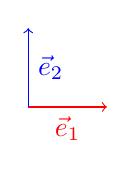
\begin{tikzpicture}
			
			\draw [->,color=red] (0,0)--(1,0) node[midway, below]{$\vec{e}_1$} ;
			\draw [->,color=blue] (0,0)--(0,1) node [right,midway]{$\vec{e}_2$};
			\end{tikzpicture}
	\end{subfigure}
	\centering
	\begin{subfigure}{0.3\textwidth}
		\begin{tikzpicture}
	
			\draw [->,thick] (0,0)--(4,0) node[midway, above]{$T$};
			\node (A) at (5,0){};
			\end{tikzpicture}
	\end{subfigure}
	\begin{subfigure}[r]{0.4\textwidth}
		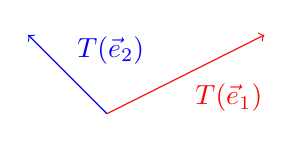
\begin{tikzpicture}
	
			\draw [->,color=red] (0,0)--(2,1) node[midway, below right ]{$T(\vec{e}_1)$} ;
			\draw [->,color=blue] (0,0)--(-1,1) node [above right ,midway]{$T(\vec{e}_2)$};
			\end{tikzpicture}
	\end{subfigure}
\end{figure}
Let us only consider the integer lattice points for now. If we start at $(a,b)$, meaning from the origin, we take $a$ steps right and $b$ steps up. In our transformed plane, we need to take $a$ steps in $(2,1)$ and $b$ steps $(-1,1)$ by linearity. We can geometrically track the place of these lattic points using a grid.
\begin{figure}[h]
	\begin{subfigure}[l]{0.4\textwidth}
		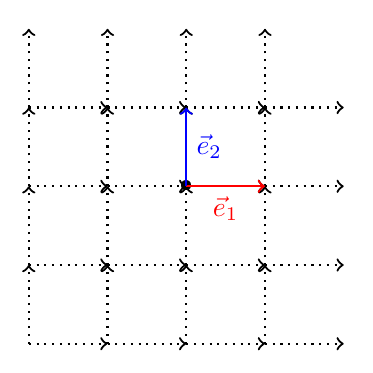
\begin{tikzpicture}
			\draw (0,0) node{\textbullet};
			\foreach \i in {-2,...,1}{
				\foreach \j in {-2,...,1}{
					\draw [->,thick,dotted] (\i,\j)--(\i+1,\j);
					
					\draw [->,thick,dotted] (\i,\j)--(\i,\j+1);
				}
			}
			\draw [->,color=red,thick] (0,0)--(1,0) node[midway, below]{$\vec{e}_1$} ;
			\draw [->,color=blue,thick] (0,0)--(0,1) node [right,midway]{$\vec{e}_2$};
			\end{tikzpicture}
			\caption{Original grid}
	\end{subfigure}
	\begin{subfigure}[r]{0.6\textwidth}
		\begin{tikzpicture}
			\draw (0,0) node{\textbullet};
			\foreach \i in {-1,...,1}{
				\foreach \j in {-1,...,1}{
					\draw [->,thick,dotted] (\i*2-\j,\j+\i)--(\i*2-\j+2,\i+\j+1);
					
					\draw [->,thick,dotted] (\i*2-\j,\j+\i)--(\i*2-\j-1,\i+\j+1);
				}
			}
			\draw [->,color=red,thick] (0,0)--(2,1) node[midway, below right ]{$T(\vec{e}_1)$} ;
			\draw [->,color=blue] (0,0)--(-1,1) node [above right ,midway,thick]{$T(\vec{e}_2)$};
			\end{tikzpicture}
			\caption{Transformed grid}
	\end{subfigure}
\end{figure}
This is just a change of our coordinate system. As long as we know where the standard basis vectors go (or any basis goes), it is enough to know the whole linear transformation. The construction is you 1. decompose any vector into the linear combination of the basis vectors, then 2. add up the corresponding linear combination of the transformed basis vectors. \textbf{This intuition of linear transformations being a shift in coordinates is very useful}, and helps transform abstract problems in linear algebra back to concrete geometry. 
\example{
	Express the linear transformations of the dot product, cross product, and projection as matrix-vector multiplications.
}
\textbf{Dot Product: }Let $\vec{v}=(v_1,\ldots,v_n)\in\reals^n$. Then $\vec{v}\cdot\vec{e}_j=v_j$. So \[\vec{v}\cdot\vec{x} = \begin{bmatrix}
	v_1 & v_2 &  \ldots & v_n
\end{bmatrix}\vec{x}\].

\textbf{Cross Product} Let $\vec{v}=(v_1,v_2,v_3)\in\reals^n$. Then \[
	\vec{v}\times\vec{x} = \begin{bmatrix}
		0 & -v_3 & v_2\\
		v_3 & 0 & -v_1\\
		-v_2 & v_1 & 0
	\end{bmatrix}\vec{x}
\]

\textbf{Projection} Let $\vec{v}=(v_1,\ldots,v_n)\in\reals^n$. Then \[
	\textrm{Proj}_{\vec{v}}(\vec{x})=\frac{1}{|\vec{v}|^2}\begin{bmatrix}
		v_1 v_1 & v_1 v_2 & \ldots & v_1 v_n \\
		v_2 v_1 & v_2 v_2 & \ldots & v_2 v_n \\
		\vdots & & \ddots & \\
		v_n v_1 & v_n v-2 & \ldots & v_n v_n
	\end{bmatrix}\vec{x}
\]
where multiplication of matrix by scalar is entry wise.
\example{
	Let $T:\reals^m\to\reals^n$, $S:\reals^n\to\reals^p$. Let $A\in M_{m\times n}, B\in M_{n\times p}$ be the matrix representations of $S$ and $T$ respectively.
	We know that the function $F:\reals^m \to \reals^p$ defined by $F(\vec{x})=S(T(\vec{x}))$ has a matrix representation. Compute this matrix.
}
The computation is not very interesting. However, you will do this until the day you drop ISP.
If we write $A=\begin{bmatrix}
	\vec{x}_1 & \ldots & \vec{x}_m
\end{bmatrix}, \vec{b}_j\in\reals^n$, then for each $\vec{e}_j\in\reals^m$ we have $A\vec{e}_j=\vec{x}_j$.
So that \[
S(T(\vec{e}_j))= S(A\vec{e}_j) = S(\vec{x}_j) = B(\vec{x}_j).
\]
The matrix is \[
\begin{bmatrix}
	B\vec{x}_1 & B\vec{x}_2 & \ldots & B\vec{x}_m
\end{bmatrix}.
\]
Now, if we forcefully write the linear transformations in matrices, we get $S(T(\vec{x}))= BA\vec{x}$. This allows us
to define the product of matrices.
\definition{Matrix Operations}{
	Let $\alpha \in\reals$, $A=\{a_{i,j}\},B=\{b_i,j\}\in M_{m\times n}(\reals)$, $C=\{c_{i,j}\}\in M_{n\times p}(\reals)$.
	We define the addition of matrices \[
	A+B=\{a_{i,j}+b_{i,j}\},
	\]
	the pointwise addition of each entry. We define the scaling of a matrix \[
	\alpha A = \{\alpha a_{i,j}\},
	\]
	the pointise scaling of each entry. We also define the product of matrices\[
	AC = \left\{\sum_{k=1}^{n}a_{i,k}c_{k_j}\right\}.
	\]
}
\begin{remark}
	The definition of matrix product is equivalent to what we got from getting the matrix from the composition of functions.
	The only difference is that we are composing a function the other way from $\reals^p\to\reals^n\to\reals^m$.
\end{remark}
\begin{remark}
	There is a mnenomic to memorize the formula for matrix product $AB$. It involves putting $A$ on the bottom left and $B$ on the top right, like so:

	\[
	\begin{array}{cc}
		&\begin{bmatrix}
			b_{1,1} & \ldots & b_{1,p}\\
			\vdots & \ddots&\\
			b_{n,1} & \ldots & b_{n,p}
		\end{bmatrix}\\
		\begin{bmatrix}
			a_{1,1} & \ldots & a_{1,n}\\
			\vdots & \ddots&\\
			a_{m,1} & \ldots & a_{m,n}
		\end{bmatrix}	& \begin{bmatrix}\\
			\textrm{product goes here}\\
			\\
		\end{bmatrix}
	\end{array}
	\]
	The product of an $m\times n$ and an $n\times p$ matrix is an $m\times p$ matrix. To find the $i,j$'th entry of the product,
	locate the $i$-th row on matrix $A$ (left) and the $j$-th column on matrix $B$ (top). Treating the row and column as vectors with $n$ entries, the dot product is the $i,j$-th entry of the product.
\end{remark}
\begin{remark}
	Viewing a column vector as a $n\times 1$ matrix, you can verify that the matrix-vector product is compatible with the products of two matrices.
\end{remark}

\proposition{
	The matrix operations satisfy the following properties:\\
	\textbf{Addition: } Let $A,B,C\in M_{m\times n}(\reals)$, then: \begin{itemize}
		\item \textit{(Associativity)} $A+(B+C)=(A+B)+C$.
		\item \textit{(Commutativity)} $A+B=B+A$.
		\item \textit{(Identity)} The zero matrix $0_{m\times n}$ satisfies $A+0_{m\times n}=A$.
	\end{itemize}
	\textbf{Scaling: } Let $\alpha,\beta\in\reals, A,B \in M_{m\times n}(\reals)$, then:\begin{itemize}
		\item \textit{(Associativity)} $\alpha(\beta)A = (\alpha\beta)A$.
		\item \textit{(Distributivity)} $(\alpha+\beta)(A+B) = \alpha A + \alpha B + \beta A + \beta B$.
	\end{itemize}
	\textbf{Multiplication: } Let $A,B \in M_{m\times n}(\reals),C,D\in M_{n\times p}(\reals), E \in M_{p\times q}(\reals)$.\\
	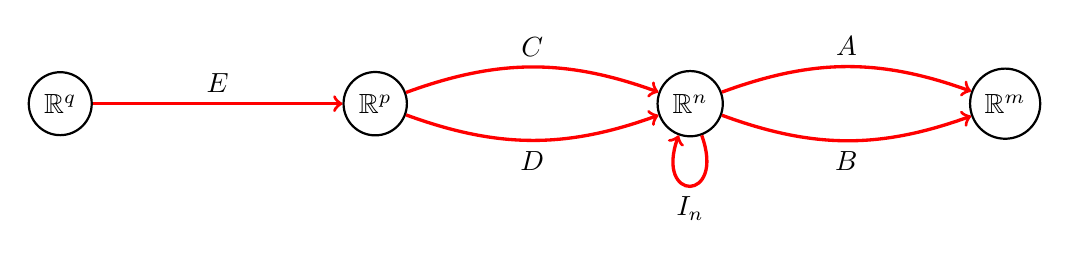
\begin{tikzpicture}
		\begin{scope}[every node/.style={circle,thick,draw}]
			\node (A) at (0,0) {$\reals^q$};
			\node (B) at (4,0) {$\reals^p$};
			\node (C) at (8,0) {$\reals^n$};
			\node (D) at (12,0) {$\reals^m$};
		\end{scope}
	
\begin{scope}[
	every edge/.style={draw=red,very thick}]
\path [->] (A) edge node [above,midway]{$E$} (B);
\path [->] (B) edge [bend left=20] node [above,midway]{$C$} (C);
\path [->] (B) edge [bend right=20]node [below,midway]{$D$} (C);

\path [->] (C) edge [in=-110, out=-70,looseness=8]node [below,midway]{$I_n$} (C);
\path [->] (C) edge [bend left=20] node [above,midway]{$A$} (D);
\path [->] (C) edge [bend right=20] node[below,midway] {$B$} (D);
\end{scope}
	\end{tikzpicture}\\
	Then \begin{itemize}
		\item \textit{(Associativity)} $A(CE)=(AC)E$.
		\item \textit{Compatibility with Scaling} $A(\alpha C)=\alpha(AC) = (\alpha A)(C)$.
		\item \textit{(Distributivity)} $(A+B)(C+D) = AC+AD+BC+BD$.
		\item \textit{(Identity)} The identity matrix $I_n \defeq \begin{bmatrix}
			\vec{e}_1 & \vec{e}_2 & \ldots & \vec{e}_n
		\end{bmatrix}$ satisfies $I_nC = C$ and $BI_n=B$.
	\end{itemize}
}
\begin{remark}
	The matrix product is generally not commutative. In fact, the product $DB$ does not make sense, because the dimensions of the matrices are not compatible!
\end{remark}
\exercises
\begin{exerciselist}
	\item Find the corresponding matrices for the following transformations: \begin{enumerate}[label=(\alph*)]
		\item 
	\end{enumerate}
	\item Find an example where \begin{enumerate}[label=(\alph*)]
		\item Two matrices $A,B\in M_{n\times n}(\reals)$ are not commutative. i.e. $AB\neq BA$.
		\item A matrix $0_{n\times n}\neq A\in M_{n\times n }(\reals)$ such that $A^k=0_{n\times n}$ for some $k>1$.
	\end{enumerate}
	\item Let $\theta,\phi\in[0,2\pi)$. Sketch how the matrix \[\begin{bmatrix}
		\cos \theta & -\sin \theta\\
		\sin \theta & \cos \theta
	\end{bmatrix}
	\] transforms the grid. Show that \[
		\begin{bmatrix}
			\cos \theta & -\sin \theta\\
			\sin \theta & \cos \theta
		\end{bmatrix}
		\begin{bmatrix}
			\cos \phi & -\sin \phi\\
			\sin \phi & \cos \phi
		\end{bmatrix}
		=
		\begin{bmatrix}
			\cos (\theta+\phi) & -\sin (\theta+\phi)\\
			\sin (\theta+\phi) & \cos (\theta+\phi)
		\end{bmatrix}
	\]
	and thus the set of matrix in this form are commutative. Is there a geometric argument for why these matrices must be commutative? 
	\item Run the following code in python multiple times and pinky promise that you got the correct answer.\\ \begin{lstlisting}[language=Python]
import numpy as np
matrix1=np.random.randint(-10,11,size=(3,3))
matrix2=np.random.randint(-10,11,size=(3,3))
print("Multiply these two matrices:")
print(matrix1,"\n",matrix2)
print("Confirm that the answer is the following:")
print(matrix1.dot(matrix2))\end{lstlisting}
\end{exerciselist}
\section{Surjective and Injective Linear Transformation}
\definition{Types of functions}{
	Let $f:U\to W$ be a function. We say $f$ is:
	\begin{itemize}
		\item \textbf{Surjective}, if the image of $U$ under $f$, $f(U)=W$. 
		This means for every $w\in W$, there is some $u\in U$ such that $f(u)=w$.
		\item \textbf{Injective}, if each $u \in U$ maps to a unique element in $W$.
		This means for every $u_1,u_2\in U$. If $f(u_1)=f(u_2)$, $u_1=u_2$. 
		\item \textbf{Bijective}, if $f$ is surjective and injective.
	\end{itemize}
}
\example{
	The following functions are surjective:\begin{itemize}
		\item The `extract' function $\Pi_j:\reals^n\to\reals$, defined by $\Pi_j(x_1,x_2,...,x_n)=x_j$ and extracts the $j$-th coordinate.
		\item The differentiation operator $\frac{d}{dx}$ from the space of \textbf{differentiable} functions to the space of \textbf{continuous} functions. This is because all continuous functions have antiderivatives.
		Moreover, as all derivatives are continuous, the differentiation operator is well defined.
		\item Integration over the interval $[0,1]$ sends the integrable function $g$ to the real number $\int_{0}^{1}g(x) \ dx$. This is surjective because the integral 
			of $g(x)=a$ over $[0,1]$ is $a$ for all $a\in \reals$.
	\end{itemize}
	The following functions are injective:\begin{itemize}
		\item The `pad zeros' function $\iota:\reals^n \to \reals^{n+1}$ defined by $\iota(x_1,...,x_n) = (x_1,...,x_n,0)$ and adds a $0$ to the final coordinate.
		\item The linear function $f:\reals \to \reals$ defined by $f(x)=2x$.
	\end{itemize}
	The following functions are surjective:\begin{itemize}
		\item The identity map $Id:\reals^n\to\reals^n$ defined by $Id(\vec{x}) = I_n \vec{x} = \vec{x}$.
	\end{itemize}
}
We can phrase these characterizations in of the number of solutions in $u$ that solve $f(u)=w$.
\proposition{
	\begin{itemize}
		\item $f$ is surjective $\iff$ $f(u)=w$ has \textit{at least one solution} in $u$ for each $w\in W$.
		\item $f$ is injective $\iff$ $f(u)=w$ has \textit{at most one solution} in $u$ for each $w\in W$.
		\item $f$ is bijective $\iff$ $f(u)=w$ has \textit{exactly one solution} in $u$ for each $w\in W$.
	\end{itemize}
}
When $f$ is a linear transformation from $\reals^n \to \reals^m$, it has a matrix representation $A\in M_{m\times n}(\reals)$.
To determine if $f$ is surjective, injective, or bijective, we look at the number of solutions in $\vec{x}$ for the equation $A\vec{x}=\vec{b}$
for each $\vec{b}\in\reals^m$.
\theorem{Surjectivity and solutions to linear systems}{
	Let $T:\reals^n\to\reals^m$, $A\in M_{m\times n}(\reals)$, and $T(\vec{x})=A\vec{x}$ for all $\vec{x}\in\reals^n$.
	Then the following are equivalent:\begin{enumerate}
		\item $T$ is surjective.
		\item $A(\vec{x})=\vec{b}$ is at least one solution in $\vec{x}$ for each $\vec{b}\in \reals^m$
		\item rref$(A)$ has a pivot in every row.
		\item The columns of $A$ span $\reals^m$.
	\end{enumerate}
}
\theorem{Injectivity and solutions to linear systems}{
	Let $T:\reals^n\to\reals^m$, $A\in M_{m\times n}(\reals)$, and $T(\vec{x})=A\vec{x}$ for all $\vec{x}\in\reals^n$.
	Then the following are equivalent:\begin{enumerate}
		\item $T$ is injective.
		\item $A(\vec{x})=\vec{b}$ is at most one solution in $\vec{x}$ for each $\vec{b}\in \reals^m$.
		\item rref$(A)$ has a pivot in every column.
		\item The columns of $A$ are linearly independent.
	\end{enumerate}
}
Again, something interesting happens when $T:\reals^n\to\reals^m$ is bijective.
This forces the matrix to be square, giving even more equivalences for That One Theorem.
\theorem{This One/ That One (Linear transformation cont.)}{
	Let $A=[\vec{v}_1\ldots \vec{v}_n]\in M_{n\times n}(\reals)$, and $T:\reals^n\to\reals^n$ be the unique linear transformation satisfying $T(\vec{x})=A\vec{x}$ for all $\vec{x}\in\reals^n$.
	Then the following are equivalent.
	\begin{enumerate}
		\item $\{\vec{v}_1,\ldots,\vec{v}_n\}$ form a basis.
		\\ $\vdots$
	\end{enumerate}
	
	\begin{thatonethmlist}
		\item $T$ is bijective.
		\item $T$ is surjective.
		\item $T$ is injective.
	\end{thatonethmlist}
}
\exercises
	%\section{Inverses and determinants}
\subsection{Inverse}
\definition{Inverse function}{
    Let $T:U\to V$ be bijective.
    The \textbf{inverse of} $T$ is the unique function $T^{-1}$ that satisfies
    \begin{align*}
        T^{-1}(T(x))= x,\\
        T(T^{-1}(y))=y
    \end{align*}
    for all $x\in U, y\in V$.\\
    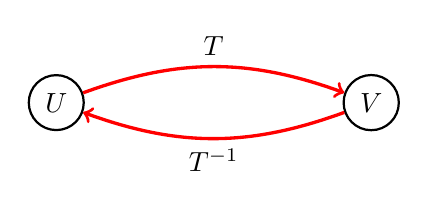
\begin{tikzpicture}
		\begin{scope}[every node/.style={circle,thick,draw}]
			\node (A) at (0,0) {$U$};
			\node (B) at (4,0) {$V$};
		\end{scope}
	
\begin{scope}[
	every edge/.style={draw=red,very thick}]
\path [->] (A) edge [bend left=20] node [above,midway]{$T$} (B);
\path [->] (B) edge [bend left=20]node [below,midway]{$T^{-1}$} (A);
\end{scope}
	\end{tikzpicture}
}
How do we know this inverse exists? We know that for each $y\in V$ there is exactly one
$x\in U$ that satisifes $T(x)=y$, so we can set $T^{-1}(y)$ to be this particular value of $x$ for each y.
This definition of the inverse sounds tautological, so let us apply this to linear transformations.
\proposition{
    Let $T:\reals^n\to\reals^n$ be a bijective linear transformation.
    Then $T^{-1}$ is a linear transformation.
}
\begin{proof}
    We want to show that for any $\vec{y}_1,\vec{y}_2\in\reals^n$, $c\in \reals$,
    $T^{-1}(\vec{y}_1+\vec{y}_2)=T^{-1}(\vec{y}_1)+T^{-1}(\vec{y}_2)$ and $T^{-1}(c\vec{y}_1)=cT^{-1}(\vec{y}_1)$.

    The trick to solving this is to use the definition for inverses and switch back and forth with $T$ and $T^{-1}$, and apply linearity of $T$.
    \begin{align*}
        T^{-1}(\vec{y}_1)+T^{-1}(\vec{y}_2) &= T^{-1}(T(T^{-1}(\vec{y}_1)+T^{-1}(\vec{y}_2)))\\
        &=T^{-1}(T(T^{-1}(\vec{y}_1))+T(T^{-1}(\vec{y}_2))) \textrm{ (as $T$ is linear)}\\
        &=T^{-1}(\vec{y}_1+\vec{y}_2).
    \end{align*}
    For scaling,\begin{align*}
        cT^{-1}(\vec{y}_1) &= T^{-1}(T(cT^{-1}(\vec{y_1})))\\
        &=T^{-1}(c(T(T^{-1}(\vec{y_1}))))\\
        &=T^{-1}(c\vec{y}_1).
    \end{align*}
\end{proof}
This means that the inverse of $T$ has a matrix representation.
If we write $T(\vec{x})=A\vec{x}$ for some matrix $A$,
then there is some matrix $B$ such that $AB=BA=I_n$.
\definition{Matrix Inverses}{
    Let $A\in M_{m\times n}(\reals)$. If there exists $X\in M_{n\times m}(\reals)$ such that
    \[
    XA=I_n,
    \]
    we call $X$ the \textbf{left inverse} of $A$.
    Similarly, if there exists $Y\in M_{n\times m}(\reals)$ such that
    \[
        AY=I_m,
    \]
    we call $Y$ the \textbf{right inverse} of $A$.
    If both the left and right inverses exist and are equal, then we say that $A$ is \textbf{invertible}, and denote $X=Y$ the \textbf{inverse} of $A$, written as $A^{-1}$.
}
\begin{remark}
    If $A$ has a left and right inverse, then the left and right inverses are equal. Indeed, we have for a left inverse $X$ and a right inverse $Y$ of $A$,\[
    X= X(I_m)= X(AY) = (XA)Y = (I_n)Y = Y.
    \]
\end{remark}
As we have already seen, only bijective linear transformations have inverses, so that means we have more to add to That One Theorem. We also see that being invertible implies having a left and right inverse, so might expect that having a left or right inverse corresponds to the columns being linearly independent or span $\reals^m$. 
\example{
    $A\in M_{m\times n}(\reals)$ having a left/right inverse indeed corresponds to the conditions that the columns are linearly independent and the columns span $\reals^m$. Figure out which conditions correspond to which.
}
There are two ways to think about this problem: one way is directly translate left and right inverses to the corresponding statements of the column vectors; the other way is to think of them in linear transformations and find out which one is surjective/injective. I will outline both methods.

\textbf{Method 1:} 
Without knowing where to go, let us suppose we want to prove $A$ has linearly independent columns and see which extra hypothesis we need. Suppose \[
    A\vec{x}=\vec{0}.
\]
We want to show $\vec{x} = \vec{0}$. This means we want to cancel the $A$ on the left, so we want to use the left inverse $X$. \[
\vec{x}=XA\vec{x} = X\vec{0} = \vec{0}.
\] 
So this means having a left inverse corresponds to linear independence.
Now to prove the columns of $A$ span $\reals^m$, we try to solve \[
A\vec{x}=\vec{b}
\] for any $\vec{b}\in\reals^m$.
To produce a solution $\vec{x}$ that can cancel $A$ from the right, we will need the right inverse $Y$, and set $\vec{x}=Y\vec{b}$, then
\[
A\vec{x}=AY\vec{b}=\vec{b}.
\]

\textbf{Method 2:}
We translate the problem into a linear transformation $T:\reals^n\to\reals^m$ being injective (linear independence) and surjective (span $\reals^m$).
Why does a left inverse imply injectivity? Let us suppose $T(\vec{x})=T(\vec{y})$, then the left inverse can immediately cancel out the $T$ from the left and give us $\vec{x}=\vec{y}$.

For surjectivity, let us break down the columns of the right inverse $Y=\begin{bmatrix}
    \vec{y}_1 & \ldots &\vec{y}_m
\end{bmatrix}$.
Then by the property of matrix multipication, we can consider each column to see \[
A\vec{y}_j = \vec{e}_j.
\]
Since the basis vectors can build anything in $\reals^m$, we can just use the corresponding linear combination of the $\vec{y}_j$'s to build anything in $\reals^m$.
This means we have three extra equivalences for a matrix being invertible.

\theorem{This/That One}{
    Let $A=[\vec{v}_1\ldots \vec{v}_n]\in M_{n\times n}(\reals)$, and $T:\reals^n\to\reals^n$ be the unique linear transformation satisfying $T(\vec{x})=A\vec{x}$ for all $\vec{x}\in\reals^n$.
	Then the following are equivalent.
	\begin{enumerate}
		\item $\{\vec{v}_1,\ldots,\vec{v}_n\}$ form a basis.
		\\ $\vdots$
	\end{enumerate}
	
	\begin{thatonethmlist}
		\item $A$ is invertible.
		\item $A$ as a left inverse.
		\item $A$ has a right inverse.
	\end{thatonethmlist}
}

Finally, we want to compute this inverse $A^{-1}$. Let us set the columns \[
A=[\vec{a}_1 \ \vec{a}_2 \ \ldots \ \vec{a}_n],\ 
A^{-1}=[\vec{b}_1 \ \vec{b}_2 \ \ldots \ \vec{b}_n],
\] 
then the condition $AA^{-1}$ translates to \begin{align*}
	A\vec{b}_1&=\vec{e}_1,\\
	A\vec{b}_2&=\vec{e}_2,\\
	&\vdots \\
	A\vec{b}_n&=\vec{e}_n.
\end{align*}
Which means we just have to solve $n$ different linear systems. We can do them all at once: by reducing the matrix \[
\begin{bmatrix}[cccc|cccc]
	\vec{a}_1 & \vec{a}_2 & \ldots &\vec{a}_n
	&\vec{b}_1 & \vec{b}_2 & \ldots &\vec{b}_n
\end{bmatrix}
\]
to rref,
we will get \[
\begin{bmatrix}[c|c]
	I_n & *
\end{bmatrix}
\]
if $A$ is invertible. The $*$ will be the solutions $\vec{b}_k$'s, which means $*$ is the inverse of $A$.

\subsection{Isomorphisms}
\definition{Isomorphism}{
	Let $T:U\to V$ be a bijective linear transformation. We call $T$ an \textbf{isomorphism} and the vector spaces $U$ and $V$ are \textbf{isomorphic}. We denote this $U\simeq V$.
}
Recall many sections ago, we said that many types of vector spaces are very similar to $\reals^n$. Now that we have defined isomorphic vector spaces, we have a concrete statement of what it means to be similar.
\theorem{Finite dimensional real vector spaces $\simeq \reals^n$ }{
Let $V$ be a finite dimensional real vector spaces. Then $V\simeq \reals^n$ for some $n\in\mathbb{N}$.
}
\begin{proof}
	Since $V$ is finite dimensional, let $\{v_1,...,v_k\}$ be a basis for $V$.
	We just need to construct an isomorphism from $\reals^n \to V$. What is an easy way to define this? We just need to define where each of the standard basis vectors $\vec{e}_j$ goes. This gives us a very natural choice to guess that the isomorphism $T:\reals^k\to V$ defined by \[
		T(\vec{e}_j)=v_j,	
	\]
	or equivalently \[
	T(\vec{x})=x_1v_1+x_2v_2+\ldots+x_kv_k
	\]
	is bijective. This is indeed bijective, which you have confirmed in a previous exercise.	
\end{proof}
\corollary{
	Let $V$ be finite dimensional. Then every basis of $V$ has the same number of vectors.
}
\begin{proof}
	Let $\{v_1,\ldots,v_k\}$ and ${w_1,\ldots, w_l}$ be two bases for $V$. Then by the construction in the previous theorem, we have $V\simeq \reals^k$ and $V\simeq \reals^l$. So $\reals^k\simeq \reals^l$ and thus $k=l$.
\end{proof}
\subsection{Determinants}
We now move towards the last equivalence for That One Theorem. Recall in the intuition behind the \hyperref[thm:2.48]{Matrix Representation of Linear Transformations}, we constructed a grid and showed that a linear transformation is a change in the coordinate system.\\
\begin{figure}[h]
	\begin{subfigure}[l]{0.4\textwidth}
		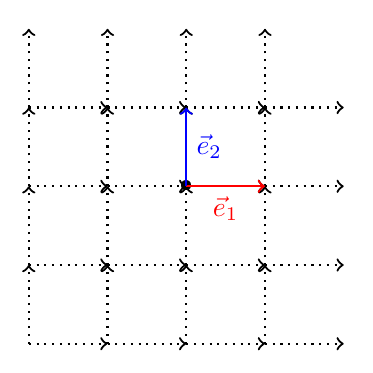
\begin{tikzpicture}
			\draw (0,0) node{\textbullet};
			\foreach \i in {-2,...,1}{
				\foreach \j in {-2,...,1}{
					\draw [->,thick,dotted] (\i,\j)--(\i+1,\j);
					
					\draw [->,thick,dotted] (\i,\j)--(\i,\j+1);
				}
			}
			\draw [->,color=red,thick] (0,0)--(1,0) node[midway, below]{$\vec{e}_1$} ;
			\draw [->,color=blue,thick] (0,0)--(0,1) node [right,midway]{$\vec{e}_2$};
			\end{tikzpicture}
			\caption{Original grid}
	\end{subfigure}
	\begin{subfigure}[r]{0.6\textwidth}
		\begin{tikzpicture}
			\draw (0,0) node{\textbullet};
			\foreach \i in {-1,...,1}{
				\foreach \j in {-1,...,1}{
					\draw [->,thick,dotted] (\i*2-\j,\j+\i)--(\i*2-\j+2,\i+\j+1);
					
					\draw [->,thick,dotted] (\i*2-\j,\j+\i)--(\i*2-\j-1,\i+\j+1);
				}
			}
			\draw [->,color=red,thick] (0,0)--(2,1) node[midway, below right ]{$T(\vec{e}_1)$} ;
			\draw [->,color=blue] (0,0)--(-1,1) node [above right ,midway,thick]{$T(\vec{e}_2)$};
			\end{tikzpicture}
			\caption{Transformed grid}
	\end{subfigure}
\end{figure}
The original grid squares become grid `parallelograms'. Indeed, if you extend to three dimensions, you can get grid `parallelepipeds'.
To say that the transformation is surjective means that the transformed unit square/cubes have non-zero area/volume and can thus tessellate.



\begin{figure}[h]
	\begin{subfigure}[l]{0.4\textwidth}
		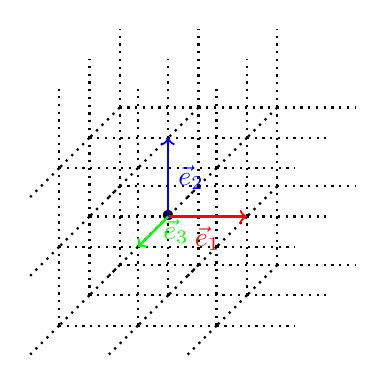
\begin{tikzpicture}
			\draw (0,0) node{\textbullet};
			\foreach \i in {-1,...,1}{
				\foreach \j in {-1,...,1}{
                    \foreach \k in {-1,...,1}{

					\draw [-,thick,dotted] (\i,\j,\k)--(\i+1,\j,\k);
					
					\draw [-,thick,dotted] (\i,\j,\k)--(\i,\j+1,\k);
					\draw [-,thick,dotted] (\i,\j,\k)--(\i,\j,\k+1);
                    }
				}
			}
			\draw [->,color=red,thick] (0,0,0)--(1,0,0) node[midway, below]{$\vec{e}_1$} ;
			\draw [->,color=blue,thick] (0,0,0)--(0,1,0) node [right,midway]{$\vec{e}_2$};
            \draw [->,color=green,thick] (0,0,0)--(0,0,1) node [right,midway]{$\vec{e}_3$};
			\end{tikzpicture}
			\caption{Original grid}
	\end{subfigure}
	\begin{subfigure}[r]{0.6\textwidth}
		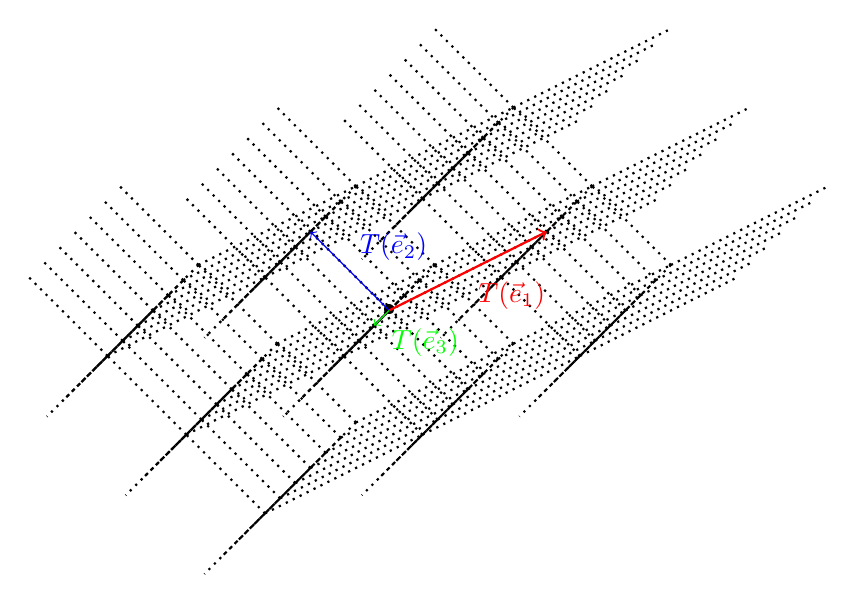
\begin{tikzpicture}
			\draw (0,0) node{\textbullet};
			\foreach \i in {-1,...,1}{
				\foreach \j in {-1,...,1}{
                    \foreach \k in {-3,...,3}{

					\draw [-,thick,dotted] (\i*2-\j,\j+\i,0.5*\k)--(\i*2-\j+2,\i+\j+1,0.5*\k);
					
					\draw [-,dotted,thick] (\i*2-\j,\j+\i,0.5*\k)--(\i*2-\j-1,\i+\j+1,0.5*\k);
					\draw [-,dotted,thick] (\i*2-\j,\j+\i,0.5*\k)--(\i*2-\j,\i+\j,0.5*\k+2);
                    }
				}
			}
			\draw [->,color=red,thick] (0,0)--(2,1) node[midway, below right ]{$T(\vec{e}_1)$} ;
			\draw [->,color=blue] (0,0)--(-1,1) node [above right ,midway,thick]{$T(\vec{e}_2)$};
			\draw [->,color=green] (0,0,0)--(0,0,0.5) node [below right,midway,thick]{$T(\vec{e}_3)$};
			\end{tikzpicture}
			\caption{Transformed grid}
	\end{subfigure}
    \caption{I tried my best, please use a bit of imagination}
\end{figure}
Here we use the god-given formula for the determinant.
\definition{Determinant}{
	We define a determinant function $\det : M_{n\times n}(\reals)\to\reals$ as follows.\begin{itemize}
		\item $\det [a] = a$ for a $1\times 1$ matrix $[a]$
		\item For higher dimensions $A = [a_{i,j}] \in M_{n\times n}(\reals)$, we recursively define \[
			\det A  = \sum_{i=1}^n (-1)^{i+j} a_{i,j} \det A_{i,j}
		\] for any $1\leq j\leq n$. Any value of $j$ will give the same formula upon expansion.
	\end{itemize}
}\begin{remark}
	$A_{i,j}$ is the the \textbf{minor} of the matrix $A$ where you delete the $i$-th row and $j$-th column.
	If \begin{align*}
	A&=\begin{bmatrix}
		a& b &*\\
		* & * & *\\
		c& d & *
	\end{bmatrix},\\
	A_{2,3}&=\begin{bmatrix}
		a&b\\c&d
	\end{bmatrix}.
	\end{align*} 
	
\end{remark}
\begin{remark}
	The recursive formula also works for 
	\[			\det A  = \sum_{i=1}^n (-1)^{i+j} a_{j,i} \det A_{j,i}
		\]
		where instead of expanding along the $j$-th row, we expand along the $j$-th column.
\end{remark}
\proposition{
	For small matrices, we have these simplified formulae.
	\begin{itemize}
		\item[$1\times 1$] $\det ([a])=a.$
		\item[$2\times 2$] $\det \left(\begin{bmatrix}
			a&b\\
			c&d
		\end{bmatrix}\right)=ad-bc$. 
		\item[$3\times 3$] $\det \left(\begin{bmatrix}
			a&b&c\\d&e&f\\g&h&i
		\end{bmatrix}\right)= aei+bfg+cdh-ceg-afh-bdi.$
	\end{itemize} 
}
\begin{remark}
	The mnenomic for memorizing the $3\times 3$ determinant is as follows:
	Extend the matrix as \[
	\begin{bmatrix}[ccc|cc]
		a&b&c&a&b\\d&e&f&d&e\\g&h&i&g&h
	\end{bmatrix}
	\]
	and take the difference between the red diagonal products and the blue diagonal products.
	\begin{figure}[h]
		\centering
		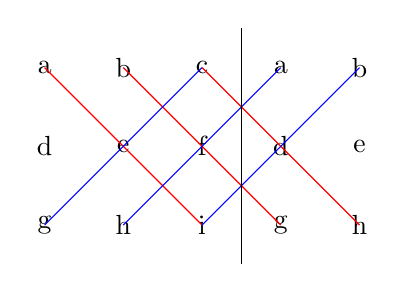
\begin{tikzpicture}
			\node (A) at (0,0) {a};
			\node (B) at (1,0) {b};
			\node (C) at (2,0) {c};
			\node (AA) at (3,0){a};
			\node (BB) at (4,0){b};
			\node (D) at (0,-1) {d};
			\node (E) at (1,-1 ){e};
			\node (F) at (2,-1){f};
			\node (DD) at (3,-1){d};
			\node (EE) at (4,-1){e};
			\node (G) at (0,-2) {g};
			\node (H) at (1,-2){h};
			\node (I) at (2,-2){i};
			\node (GG) at (3,-2){g};
			\node (HH) at (4,-2){h};
	
			\draw[-,color=red] (0,0)--(2,-2);
			\draw[-,color=red] (1,0)--(3,-2);
			\draw[-,color=red] (2,0)--(4,-2);
			\draw[-,color=blue] (2,0)--(0,-2);
			\draw[-,color=blue] (3,0)--(1,-2);
			\draw[-,color=blue] (4,0)--(2,-2);
			\draw[-,color=black] (2.5,0.5)--(2.5,-2.5);
		\end{tikzpicture}
	\end{figure}
	
\end{remark}
As you have seen in a previous chapter, the formula for the determinant of a $3\times 3$ matrix coincides with the volume of the parallelepiped spanned by the column vectors.


\example{
	Calculate the determinant of the rotational matrix \[
	R_\theta=
	\begin{bmatrix}
		\cos\theta &-\sin \theta \\
		\sin \theta&\cos \theta
	\end{bmatrix}\].
}
We just put this in the formula to get \[
	\det R = \cos^2\theta - (-\sin^2\theta) = \cos^2\theta + \sin^2\theta = 1
\]
regardles of the value of $\theta$.
\example{
	Calculate the determinant of an upper-triangular matrix in the form \[
	U=\begin{bmatrix}
		a_1& *& *&\ldots& *\\
		0 & a_2 & *& \ldots&*\\
		0&0&a_3& \ldots & * \\
		\vdots & & &\ddots& \\
		0 & 0 & 0 & \ldots & a_n
	\end{bmatrix}\in M_{n\times n}(\reals).
	\]
}
Let's consider the special case $n=3$. We do not know the values of $*$, but if we write out \[
	\begin{bmatrix}[ccc|cc]
		a_1&*&*&a_1&*\\0&a_2&*&0&a_2\\0&0&a_3&0&0
	\end{bmatrix},\]
the only diagonal that can possible have all non-zero entries gives the product $abc$. So the determinant of a triangular matrix is always the product of the diagonal terms.
The determinant of an upper triangular matrix is always the product of the diagonal terms. To show this, we need to exploit the recursive formula for the determinant.
If we expand along the first column, most of the terms in the sum are $0$, except the first term that gives \[
	(-1)^{1+1} a_1 \det \left( \begin{bmatrix}
		 a_2 & *& \ldots&*\\
		0&a_3& \ldots & * \\
		\vdots  & &\ddots& \\
		 0 & 0 & \ldots & a_n
	\end{bmatrix}\right),
\]
which is $a_1$ times the determinant of a smaller upper triangular matrix. If we know that this $(n-1)\times (n-1)$ matrix has determinant $a_2a_3\ldots a_n$, this will prove the formula for a $n\times n$ matrix, then this result will prove the formula for a $(n+1)\times (n+1)$ matrix and so on! This technique is known as Mathematical Induction. If you want to prove a statement is true for all natural numbers $n$, you can show that it is true when $n=1$, and show that if the statement is true for $n=k$, it is also true for $n=k+1$.
\begin{proof}
	We show that the determinant of $U$ is $(a_1\ldots a_n)$ by induction on the value of $n$.

	\textit{Base Case:} The determinant of the matrix $[a_1]$ is $a_1$, which is evidently the product of all the diagonal terms.
	
	\textit{Induction step:} Suppose the determinant of a $k\times k$ upper triangular matrix is the product of the diagonal terms. We compute the determinant of a $(k+1)\times (k+1)$ matrix in the form
	\begin{align*}
		U=[u_{i,j}]=\begin{bmatrix}
			a_1& *& *&\ldots& *\\
			0 & a_2 & *& \ldots&*\\
			0&0&a_3& \ldots & * \\
			\vdots & & &\ddots& \\
			0 & 0 & 0 & \ldots & a_{k+1}
		\end{bmatrix}.
	\end{align*}
	Applying the recursive formula and expanding along the first column, the only non-zero $u_{j,1}$ term is $u_{1,1}=a_1$, so \begin{align*}
		\det U &= (-1)^{1+1} a_1 \det \left( \begin{bmatrix}
			a_2 & *& \ldots&*\\
		   0&a_3& \ldots & * \\
		   \vdots  & &\ddots& \\
			0 & 0 & \ldots & a_{k+1}
	   \end{bmatrix}\right)\\
	   &= a_1 (a_2 a_3\ldots a_{k+1}) 
	\end{align*}
	by applying the hypothesis on the $k\times k$ upper triangular matrix. Then the determinant of a $(k+1)\times (k+1)$ matrix is the product of the diagonal terms. 
	By the Principle of Mathematical Induction, the determinant of an upper triangular matrix of any size is the product of its diagonal terms.
\end{proof}


\proposition{
	The elementary row operations change the determinant of a matrix in the following way:\begin{itemize}
		\item \textit{(Row Swap)} The determinant is multiplied by $-1$.
		\item \textit{(Scaling)} The determinant is multiplied by the scaling constant.
		\item \textit{(Sum)} The determinant does not change.  
	\end{itemize}
}
The proof of this is not very enlightening, so we will skip it. It boils down to working with the general determinant formula and doing intense algebra manipulation.

However, we have the following corollary 
\corollary{
	The determinant of a matrix can be computed as follows:\begin{enumerate}
		\item Reduce the matrix to rref (or row echelon form).
		\item Take the product of the diagonal terms.
		\item Multiply this product by $1/c$ for every time you scaled a row by $c$ in computing the rref.
		\item Multiply this product by $-1$ for every time you swaped two rows in computing the rref.
		\item The final product is the determinant of the matrix.
	\end{enumerate}
}
\theorem{This/That One (Determinants)}{

Let $A=[\vec{v}_1\ldots \vec{v}_n]\in M_{n\times n}(\reals)$, and $T:\reals^n\to\reals^n$ be the unique linear transformation satisfying $T(\vec{x})=A\vec{x}$ for all $\vec{x}\in\reals^n$.
	Then the following are equivalent.
	\begin{enumerate}
		\item $\{\vec{v}_1,\ldots,\vec{v}_n\}$ form a basis.
		\\ $\vdots$
	\end{enumerate}
	
	\begin{thatonethmlist}
		\item $\det A \neq 0.$ 
	\end{thatonethmlist}
}
\begin{proof}
	Recall the motivation for introducing the determinant is the signed n-dimensional volume of the paralellotope formed by the column vectors. If (and only if) the volume is non-zero, they can tesselate the whole $\reals^n$ space.

	To show the equivalence of det$A\neq 0$, we can use the condition from That One Theorem that rref$(A)=I_n$, and the previous corollary for computing determinants. If the determinant is $0$, then the product of the diagonal terms of rref$A$ has a zero, so rref$(A)\neq I_n$. On the converse, if the determinant is non-zero, all the diagonal terms in rref$(A)$ are non-zero. The only way this can happen for a matrix in rref is when the matrix is also the identity matrix.
\end{proof}


		
	\chapter{Taylor's Theorem}
    \setcounter{exercisecounter}{0}

\setcounter{thmcounter}{1}
 \section{Analytic Functions and Taylor Series}
In this section we look to develop a method to represent functions as series. An important application of such is the use of series as solutions to differential equations. 

\definition{Power Series}{
    Let $x_0\in \reals$. A \textbf{power series} cenetered at $x_0$ is in the form \[
        f(x)=\sum_{n=0}^{\infty} a_n(x-x_0)^n.
    \]
}
\begin{remark}
    The convention used for $0^0$ when $x=x_0$ here is $0^0=1$. You can imagine that it is the limit of $(x-x_0)^0$ as $x\to x_0$.
\end{remark}
\begin{remark}
    The series might not converge. In fact, the root test for convergence gives an exact criteria for convergence.
\end{remark}
\definition{Radius of Convergence}{
    Let $f(x)$ be a power series centered at $x_0$. The \textbf{radius of convergence} is the value $R$ such that \[
    \begin{cases}
        f(x) \textrm{ converges, } & \textrm{ if $|x-x_0|<R$},\\
        f(x) \textrm{ diverges, } & \textrm{ if $|x-x_0|>R$}.
    \end{cases}
    \]
}
\definition{Analytic Functions}{
Let $\Omega \subseteq \reals$ be open, and $f:\Omega\to\reals$. We say that $f$ is \textbf{analytic} at $x_0$ if there exists $\epsilon>0$, and a power series representation $p_{x_0}(x) = \sum_n a_n(x-x_0)^n$ such that $p_{x_0}(x)$ converges to $f(x)$ in $B(x_0,\epsilon)$. We say that $f$ is analytic on (a,b) if $f$ is analytic at every point in $(a,b)$.
}
\proposition{
    The set of points on which $f$ is analytic form an open set.
}
Being analytic is one of the strictest properties for a function. Analytic functions are infinitely differentiable (smooth).

\theorem{Analytic Functions are Smooth}{Suppose $\sum a_nx^n$ is a power series representation for some function $f$ with a radius of convergence $R > 0$. Then $f$ is infinitely differentiable on $(-R, R)$. }
The proof requires some analysis knowledge out of scope of the course. The hardest part is to show that you can differentiate under the summation, i.e. \[
\frac{d}{dx}\sum_n {f_n(x)} = \sum_n \frac{d}{dx} f_n(x).
\]
Assuming this, we can get power series representations for $f'(x)$ and so on.
\begin{align*}
    \begin{array}{ccccccc}
    f(x) =&  a_0 &+ a_1(x-x_0) &+ a_2(x-x_0)^2 &+a_3(x-x_0)^3&+a_4(x-x_0)^4& +\ldots \\
    f'(x)=&   &a_1 &+ 2a_2(x-x_0) &+ 3a_3(x-x_0)^2 &+4a_4(x-x_0)^3 &+\ldots \\
    f''(x)=& &   &2a_2 &+ 6a_3(x-x_0) &+ 12a_4(x-x_0)^2&+\ldots
    \end{array}
\end{align*}
Importantly, these have the same radius of convergence as the original function (a root test can confirm this), so we get a closed form for the $k$-th derivative of $f$:
\[f^{(k)}(x) = \sum_{n=k}^{\infty} \frac{n!}{(n-k)!}a_n(x-x_0)^{n-k} \] 

\theorem{Uniqueness of Power Series}{
    Let $f$ be analytic at $x_0$. Then its power series representation $\sum_n a_n (x-x_0)^n$ is unique with coefficients
    \[a_k = \frac{f^{(k)}(x_0)}{k!}.\]}

\begin{proof}
    We take the general form of the $k$-th derivative, and evaluate it at $x=x_0$.
    This gives us \[
    f^{(k)}(x_0)=\sum_{n=k}^{\infty} \frac{n!}{(n-k)!}a_n(x_0-x_0)^{n-k}.
    \]
    On the right hand side, all the terms with $n>k$ will evaluate to $0$. The term with $n=k$ evaluates to $k!a_k$. This means \[
    f^{(k)}(x_0) = k! a_k \implies a_k = \frac{f^{(k)}(x_0)}{k!}.
    \]
    Therefore, if a power series exists, it must be in the form \[
    \sum_n \frac{f^{(n)}(x_0)}{n!} (x-x_0).
    \]
\end{proof}
\definition{Taylor Series}{The \textbf{Taylor expansion} of $f$ centered at $x_o$ is given by
\[f(x) = \sum_{n=0}^{\infty} \frac{f^{(n)}(x_o)}{n!}(x-x_o)^n.\]}

A function locally equals to its Taylor series (about some point) if and only if it is analytic. We will see that if a function is analytic, it is equal to the Taylor series about a point everywhere the series converges.
\theorem{Uniqueness of Analytic Functions}{
    Let $f,g:(a,b)\to\reals$ be analytic. Suppose $f(x)=g(x)$ on some small ball $B(x_0,\epsilon)$. Then $f=g$ everywhere on $(a,b)$.
}

    Let's consider the function $h(x)=f(x)-g(x)$. This is analytic, as we can just take the difference of the respective coefficients in the power series for $f$ and $g$. We have $h(x)=0$ on $B(x_0,\epsilon)$. Our task now is to show that $h(x)=0$ everywhere, so $f=g$ everywhere.

    The idea now is to start with the power series about $x=x_0$ \[
    \sum_{n} 0 (x-x_0)^n.
    \]
    We can `slide' this $x_0$ across a little bit to $x_1\in B(x_0,\epsilon)$ to get \[
        \sum_{n} 0 (x+x_1-x_0-x_1)^n =\sum_{n} 0 (x-x_1)^n 
    \]
    after binomial expansion of the terms $((x-x_1)+(x_1-x_0))^n$. Since $f$ is analytic at $x_1$, there is another ball centered at $x_1$ where $h=0$. Therefore, we can `slide' our center of the power series from $x_1$ to another $x_2$. If we can slide this to everywhere in $(a,b)$ we will get that the power series representation at every point is $0$. 

    \textit{optional material:} How do we guarantee that we can slide everywhere? This requires another idea from analysis called compactness. In short, the compactness of the interval $[x_0,\tilde{x}]$ or $[\tilde{x},x_0]$ guarantees that we can slide our center of the power series across from $x_0$ to any $\tilde{x}\in (a,b)$ in a finite amount of steps. 

    We will give another way to prove this, as we have introduced Zorn's lemma. Without loss of generality, let $x_0<\tilde{x}\in (a,b)$ Consider $S$, the set of points $x\leq \tilde{x}$ that you can `slide to' from $x_0$ in a finite amount of steps. I claim that every increasing sequence in $S$ is bounded above by some element in $S$.
    Let $x_1\leq x_2\leq x_3 \leq \ldots$ be an increasing sequence in $S$. We take $y=\lim_{n\to\infty} x_n$, then the series is bounded above by $y$. To construct the finite sequence going from $x_0$ to $y$, we see that $f$ is analytic at $y$ thus it has a power series representation centered at $y$ that converges to $f$ for some $B(y,\delta)$. We take $m$ large such that $x_m>y-\delta/4$. If we slide the power series centered at $y$ to be centered at $x_m$, the power series converges to $f$ at least in $B(x_m,3\delta/4)\ni y$. That is, you can recenter the power series from $x_m$ to $y$. Therefore, we take the finite sequence that recenters the power series at $x_0$ to $x_m$, then recenter that sequence at $y$. Therefore $S$ contains a maximal element by Zorn's lemma. Finally, to find out what this maximal element is, we make use of the fact that the points where $f$ is analytic is open. Therefore, the only point that can be the maximal element of $S$ is $\tilde{x}$, which is used as the upper limit of all elements in $S$. Therefore $\tilde{x}$ is the maximal element in $S$, thus $f=0$ in some ball centered at $\tilde{x}$. We picked $\tilde{x}$ to be arbitrary, so $f=0$ everywhere in $(a,b)$.

\corollary{
    Let $x_0\in (a,b)$, and $f$ is analytic on $(a,b)$, $f$ equals the power series centered at $x_0$ where the power series converges.
}
\begin{proof}
    The power series is analytic, and equals $f$ on some small open ball in $(a,b)$.
\end{proof}
\exercises
\begin{exerciselist}
    \item Find the Taylor Series for the given functions at the indicated points. \begin{enumerate}[label=(\alph*)]
        \item $f(x) = e^{-x}, x_0 = 0.$
        \item $f(x) = e^x, x_0 = 1.$ 
        \item $f(x)=1/x, x_0 = 1.$
        \item $f(x) = \cos(x), x_0 = \pi/2.$ 
        \item $f(x) = \ln(x), x_0 = 1.$
    \end{enumerate}
    \item Determine the radius of convergence of the given function about $x=0$. \begin{enumerate}[label=(\alph*)]
        \item $f(x) = (1+x)/(x-2).$
        \item $f(x) = 2x/(1+2x^2).$
        \item $f(x) = 1/(1-t^3).$
        \item $f(x) = ((t-4)(t^2+3))^{-1}.$
    \end{enumerate} 
\end{exerciselist}

\section{Taylor's Theorem with Remainder}
Sometimes we don't want to take the whole power series representation, but truncate the series to get an approximation for the functions.

\todo show that the n-th order taylor series is the best n-th order approximation for a function.
As Taylor Series are used to approximate functions, it is of relevance to determine the accuracy of a series in representing its desired function. 
\definition{Taylor's Formula with Remainder}{The remainder of order n of the Taylor expansion of $f(x_o)$ is represented by the function,
\[R_n(x) = f(x) - \sum_{k=0}^{n-1} \frac{f^{(k)}(x_o)}{k!}(x-x_o)^k.\]
}
The remainder of a Taylor expansion is the difference between the value of a function $f$ at $x$ and the partial sum of the $n^{th}$ term Taylor series. The series converges if $\lim_{n \rightarrow \infty} R_n = 0$. 

\theorem{}{Let $f(x)$ be a function on the interval $(a,b)$. $f$ is analytic on $(a,b)$ if there exists and $M>0$ such that 
\[|f^{(n)}(x) \leq M^n\]
for all $x \in (a,b)$ and $n \in \mathbb{N}$. 
}
As a result of this theorem, the Taylor series expansion holds for all $x \in (a,b)$.
\proof{Let $f(x)$ be a function on the interval $(a,b)$ and $x_o \in (a,b)$. For some $M \in \reals$ set $C = max{M|a-x_o, M|b-x_o|}$. Then the $n^{th}$ term remainder of the Taylor expansion of $f(x)$ at $x_o$ is given by
\[R_n = f(x) - \sum_{k=0}^{n-1}\frac{f^{(k)}(x_o)}{k!}(x-x_o)^k = \sum_{k=n}^{\infty} \frac{f^{(k)}(x_o)}{k!}(x-x_o)^k \]
Each term in this infinite series for $R_n$ is given by
\[R_k = \frac{f^{(k)}(x_o)}{k!}(x-x_o)^k \leq \frac{M^k}{k!}\]}

\section{Multidimesnional Taylor Series}
We look to extend the formulation for the Taylor series to approximate functions of multiple variables. 
\definition{}

\section{Extrema of Multivariate Functions}
Just as we are interested in finding the extreme points of functions of a single variable, we likewise wish to solve for stationary points of multivariate functions. Analysis of functions of multiple variables have analogous first and second derivative tests to those learned in single variable calculus. I used the term 'stationary point' as in three dimensions in addition to maxima or minima there exist so called 
saddle points. A 3D representation of a saddle point is presented in figure 
\definition{Multivariable First Derivative Test} {A point $(x_o, y_o) \in \mathbb{R^2}$ is a \textit{stationary point} of some function $f(x,y)$ if
\[\nabla f \rvert_{(x, y) = (x_o, y_o)} = 0\]}
Also similarly to the second derivative test in single variable calculus, we also have an analogous second derivative test in multivariable calculus to determine the classification of critical points. For this we use the discussion of multivariable Taylor series discussed in section . To second order, the Taylor expansion of some function $f(x,y)$ around $(x_o, y_o)$ is
\[f(x,y) \approx f(x_o, y_o) + \nabla f(x_o, y_o)^T d + \frac{1}{2!}d^THf(x_o,y_o)d + R_2(x,y)\]
From the first derivative test $\nabla f(x_o, y_o) = 0$ thereby eliminating that term. Also, we know $R_2 \rightarrow 0, (x,y) \rightarrow (x_o, y_o)$. Thus we have
\[f(x,y) \approx f(x_o, y_o) + \frac{1}{2!}d^THf(x_o,y_o)d \]
Rearranging we have 
\[f(x,y) - f(x_o, y_o) = \frac{1}{2!}d^THf(x_o,y_o)d \]
The left side appears as the numerator of the definition of the derivative. The sign of our derivative is dependent on the Hessian matrix $H$ which holds for all points $(x,y)$ near $(x_o, y_o)$. 
\section{Lagrange Multipliers}


	
\chapter{First Order Differential Equations}
\setcounter{exercisecounter}{0}

\setcounter{thmcounter}{1}
\section{Introduction}
A differential equation is an equation that relates an undetermined function with one or more of its derivatives. We call equations involving only single-variable derivatives of functions \textit{ordinary differential equations} (ODEs) and those containing partial derivatives of multivariable functions \textit{partial differential equations}(PDEs). We will focus on the former in this course and leave study of the latter to MATH 381. \newline
\newline
The highest order derivative occurring in an ODE defines the \textit{order} of the differential equation. We will look at first and second order ordinary differential equations. ODEs can be either homogeneous or inhomogeneous. Homogeneous equations have all terms involving the function $y$ or derivatives of $y$ summed to equal $0$, while inhomogeneous equations will sum to equal a nonzero term. 
\[\mbox{Homogeneous}: f(y, y',...,y^n, t) = 0\]
\[\mbox{Inhomogeneous}: f(y, y',...,y^n) = g(t)\]
\newline
Another classification of differential equations is concerned with the linearity of the terms. We can have either linear or nonlinear equations. An ODE
\[f(y, y',...y^n,t) = g(t)\]
is linear if $f$ is linear with respect to terms involving the variable $y$ or derivatives of $y$. The general form looks like
\[a_0(t)y^n+....+a_n(t)y = g(t)\]
Nonlinear equations will typically have terms involving $y$ or derivatives of $y$ multiplied together or terms involving nonlinear functions of $y$ such as $sin(y)$ or $e^y$.
\newline


\section{Separation of Variables}
A separable differential equation is any differential equation of the form,
\[N(y)\frac{dy}{dt} = M(t)\]
This allows us to multiply across by $dt$ and integrate both sides to find a function $y(t)$. 
\[\int N(y(t))\frac{dy}{dt}dt = \int M(t)dt\]
I have written $N(y) = N(y(t))$ since $y$ is a function of $t$. Then we can suppose that $\frac{d}{dt}(y(t)) = N(y(t))\frac{dy}{dt}$. Which leads to the conclusion
\[y(t) = \int M(t)dt + C\]
for some constant $C$. You may have seen the differential treated as a fraction that can be separated and while that is sufficient for all computation purposes and will lead to the same answer, the formulation above is more mathematically rigorous. 

\section{Differential Forms}
Differential forms are generalized methods for describing derivatives and integrals in multi-dimensional spaces.
Suppose we have the differential equation
\[\frac{dy}{dx} = f(x,y)\]
We can convert this equality into the form
\[Mdx + Ndy = 0\]
setting $f(x,y) = \frac{-M(x,y)}{N(x,y)}$.
Solutions to each of these forms while conveying the same information, can be interpreted in different ways. A solution $f(x)$ to () is a collection of functions satisfying the differential equation, each corresponding to a different initial condition. A solution $f(x,y) = c$ to () is a collection of level curves in $\mathbf{R}^2$. Each $f(x)$ is a subset of one of the level curves $f(x,y) = c$. 
\newline
\hfill \break
Along a curve $C$, we can write $ d\vec{r} = \langle dx, dy \rangle$ which points in the tangential direction. Similarly, we can define $F = \langle M, N \rangle$. Thus equation () can be rephrased as $F \cdot d\vec{r}$. \\
\hfill \break

\section{Integration Factors}






\section{Variation of Parameters}
Following our discussion of first order homogeneous differential equations, we now move on to discussing methods of findings solutions to inhomogeneous first order differential equations.
\[\frac{dy}{dx} + a(x)y = b(x)\]
We propose a solution $y(x) = u(x)h(x)$ where $h(x)$ is the solution to the corresponding homogeneous equation.
\[\frac{dy}{dx} +a(x)y = 0\]
The solution to this equation is
\[h(x) = e^{-\int a(x)dx}\]
Going back to our solution form $y(x) = u(x)h(x)$ and substituting into our inhomogeneous equation
\[\frac{du}{dx}h + u\frac{dh}{dx} + a(x)uh = b(x)\]
\[\frac{du}{dx}h + u\left( \frac{dh}{dx} + a(x)h \right) = b(x)\]
Since $h(x)$ is a solution to the homogeneous equation, the term in the parenthesis vanish. Therefore our differential equation becomes
\[\frac{du}{dx} = \frac{b}{h}\]
Solving for $u$ we get
\[u = \int \frac{b(x)}{h(x)}dx\]
Lastly, multiplying by $h(x)$ to get our full solution $y(x)$
\[y(x) = h(x)\left(\int \frac{b(x)}{h(x)}dx + C\right)\]
Notice here that I have already included the constant of integration here. This is because the method of solving inhomogeneous differential equations often settles down to combining a general and particular solution. We see that the constant multiplied by $h(x)$ will give us a general solution to the homogeneous equation while the product of the term in the integral and $h(x)$ will give a particular solution. 


\section{Existence and Uniqueness}

	
\chapter{Second Order Differential Equations}
\setcounter{exercisecounter}{0}

\setcounter{thmcounter}{1}
\section{Introduction}
\section{Constant Coefficients}
The first technique we will study in solving second order differential equations is for cases of homogeneous equations with constant coefficients. Such equations are of the form 
\[ay'' + by' + cy = 0\]
This equation suggests we are looking for solutions $y(t)$ for which the derivatives can be easily summed together to produce zero. Methods in calculus suggests the solution
\[y(t) = e^{rt}\]
Let's suppose this is the case, then
\[y'(t) = re^{rt}\]
\[y''(t) = r^2e^{rt}\]
Substituting these into our differential equation
\[a(r^2e^{rt}) + b(re^{rt}) + c(e^{rt}) = 0\]
\[(ar^2 + br + c)e^{rt} = 0\]
Since $e^{rt} \neq 0$, this implies we want to find values $r$ which satisfy 
\[ar^2 + br + c = 0\]
The fundamental theorem of algebra states that solving this equation will produce at least one complex root and 2 roots total counted for multiplicity. In this section, we will look at this case in which the equation produces two roots distinct $r_1, r_2 \in \mathbb{R}$. Thus we get two solutions, 
\[y_1 = e^{r_1t}\]
\[y_2 = e^{r_2t}\]
We check linear independence with the Wronskian,
\[\begin{vmatrix}
e^{r_1t} & e^{r_2t} \\
r_1e^{r_1t} & r_2e^{r_2t} \\
\end{vmatrix} = r_2e^{r_1}e^{r_2} - r_1e^{r_1t}e^{r_2t} = (r_2-r_1)e^{r_1+r_2)t} \neq 0 \]
since the exponential function is never zero and $r_1, r_2$ are distinct.
This gives us two linearly independent solutions that produce a basis for the set of solutions to this differential equation, thus our general solution is
\[y = c_1e^{r_1t} + c_2e^{r_2t}\]
where $c_1, c_2$ are undetermined coefficients to be determined by initial conditions. 


\section{Complex Roots}
We now look at cases of equations in the previous section for which the characteristic equation produces complex roots. However, a quick remark is needed first. 
\definition{Make this a remark somehow}{A polynomial of degree 2 with real coefficients can either have, 2 real, 2 complex, 1 repeated real or 1 repeated complex roots.}
This means that any degree two polynomial cannot have one real root and one complex root. We will now look at cases for which we have two complex roots. 
Suppose we have a differential equation of the form
\[ay'' + by' + cy = 0\]
The previous section suggests we solve the quadratic equation
\[ar^2 + br+ c = 0\] 
to find $r_1$ and $r_2$ that produce solutions $y_1 = e^{r_1t}$ and $y_2 = e^{r_2t}$ to the differential equation. If
\[r_1 = a_1 + b_1i\]
\[r_2 = a_2 + b_2i\]
then our general solution becomes
\[y = c_1e^{(a_1+b_1i)t} + c_2e^{(a_2+b_2i)t}\]
However, certain cases prove it useful to find real solutions. 
In these cases we use Euler's Identity 
\[e^{(a+bi)t} = e^{at}(cos(bt) + isin(bt))\].
The power in this technique is that it produces two real solutions from a single complex solution. We will prove this now.
\proof{
Suppose $y = u + iv$ is a complex solution to the second order homogeneous differential equation with constant coefficients 
\[ay''+by'+cy=0\]
where $u$ and $v$ are real valued functions.
We have
\[y' = u' + iv'\]
\[y''=u''+iv''\]
Substituting into our differential equation
\[a(u''+iv'')+b(u'+iv')+c(u+iv)=0\]
\[= (au''+bu'+u)+i(av''+bv'+cv)=0\]
This suggests both the real and imaginary parts of this equation must be zero thus we have,
\[au''+bu'+cu =0\]
\[i(av''+bv'+cv)=0\]
This results suggests that both $u$ and $v$ are real solutions to the differential equation. 
}
Now if we let $u = cos(bt)$ and $v = sin(bt)$ we have obtained two real solutions to our differential equation from one complex solution. We still must have the $e^at$ factor multiplied by $u+v$ and our two undetermined coefficients to be satisfied by initial conditions; therefore our general solution is
\[y = e^{at}(c_1cos(bt) + c_2sin(bt))\]
We check linear independence with the Wronskian
\[\begin{vmatrix}
    
\end{vmatrix}\]
From this result we see that for cases of complex roots only one root suffices to obtain a general solution. 

\section{Method of Reduction of Order}
When our characteristic equations of second-order constant coefficient homogeneous equations results in repeated roots, we obtain only one solution. Therefore we look to develop a technique to find a second solution. We suggest a solution of the form 
\[y(t) = v(t)y_1(t)\]
where $y_1(t)$ is the first solution found. 
Taking derivatives we have
\[y'(t) = v'(t)y_1(t) + v(t)y'_1(t)\]
\[y''(t) = v''(t)y_1(t) + 2v'(t)y'_1(t) + v(t)y''_1(t)\]
Substituting this into the differential equation to solve for the undetermined equation $v(t)$
\[ay''+by'+cy = 0 \]
\[a(v''y_1 + 2v'y'_1 + vy''_1) + b(v'y_1 + v'y'_1) + c(vy_1) = 0 \]
\[av''y_1 + v'(2ay'_1+by_1) + v(ay''_1 + by'_1 + cy_1) = 0\]
The third term is zero since $y_1$ is a solution to that differential equation which is the same as what we started out with. Therefore we have
\[av''y_1 + v'(2ay'_1+by_1)=0\]
\[\frac{v''}{v'} = \frac{-(2ay'_1+by_1)}{ay_1}\]
We can solve this separable differential equation for $v'$
\[\int \frac{dv}{v} = \int (-\frac{2y'_1}{y_1} - \frac{b}{a})dt\]
This gives us the solution
\[v' =\frac{1}{y_1^2}Ce^{-\int \frac{b}{a}dt}\]
We have kept the argument in the exponential in integral form as this method is generalizable to any differential equation in which we have one solution and require another for a general solution, however, in the case of constant coefficients the exponential will be $e^{bt/a}$.


\section{Variation of Parameters}
Thus far we have developed techniques to solving homogeneous second order equations. We now turn our attention to finding methods to solve inhomogeneous equations.
\[ay''+by'+cy = f(t)\]
We find solutions to inhomogeneous equations by adding a general solution to the corresponding inhomogeneous equation with a particular solution to the inhomogeneous equation. 
\[y = y_g + y_p\]
Suppose we can find two linearly independent solutions to the corresponding homogeneous equation of (), $y_1, y_2$. The method of variation of parameters suggests we look for a particular solution of the form
\[y(t)_p = u(t)y_1(t)+u_2(t)y_2(t)\]
where $y_1(t), y_2(t)$ are solutions to the corresponding homogeneous equation and $u_1(t), u_2(t)$ are undetermined coefficients. 
Taking the derivative
\[y' = u'_1y_1+u_1y'_1 + u'_2y_2+u_2y'_2\]
These calculations are made simpler if we set 
\[u'_1y_1 + u'_2y_2 = 0 \]
Therefore $y'$ becomes
\[y' = u_1y'_1 + u_2y'_2 \]
Finding $y''$
\[y'' = u'_1y'_1 + u_1y''_1 + u'_2y'_2+u_2y''_2\]
Substituting this into our differential equation
\[a(u'_1y'_1 + u_1y''_1 + u'_2y'_2+u_2y''_2)+ b(u_1y'_1 + u_2y'_2 )+c(u_1y_1 + u_2y_2) = f(t)\]
\[u_1(ay''_1 + by'_1+cy_1) + u_2(ay''_2 + by'_2+cy_2) + au'_1y'_1+au'_2y'_2 = f(t) \]
Since $y_1$ and $y_2$ are solutions to the corresponding homogeneous equation, the first two terms are zero. Thus, our equation reduces to
\[au'_1y'_1+au'_2y'_2 = f(t)\]
We now have two equations and two unknowns.
\[u'_1y_1 + u'_2y_2 = 0 \]
\[au'_1y'_1+au'_2y'_2 = f(t)\]
From this we obtain
\[u'_1 = \frac{-y_2f(t)/a}{y_1y'_2 - y'_1y_2}\]
\[u'_2 = \frac{y_1f(t)/a}{y_1y'_2 - y'_1y_2}\]
We can integrate to find $u_1$ and $u_2$.
\[u_1 = \int \frac{-y_2f(t)/a}{y_1y'_2 - y'_1y_2} dt\]
\[u_2 = \int \frac{y_1f(t)/a}{y_1y'_2 - y'_1y_2} dt \]
You may notice that the argument in the denominator is the Wronksian thereby implying that if our solutions $y_1, y_2$ are not linearly independent, then when don't have the requisite information to form a general solution to the differential equation. It that case we must return to section 3.5 and find a second linearly independent equation via Method of Reduction of Order. 
\linebreak
\linebreak
This provides us with our particular solution to the inhomogeneous differential equation
\[y_p = y_1\int \frac{-y_2f(t)/a}{y_1y'_2 - y'_1y_2} dt + y_2\int \frac{y_1f(t)/a}{y_1y'_2 - y'_1y_2} dt\]



\section{Method of Undetermined Coefficients}
There are certain classes of inhomogeneous equations such that we can propose a solution form and algebraically solve for specifying parameters. Such classes usually involve equations of constant coefficients and inhomogeneous terms of familiar functions like exponentials or sinusoidals. As in the previous section, to find a full solution to an inhomogeneous equation we sum together a general solution to the corresponding homogeneous equation with a particular solution to the inhomogeneous equation. Suppose we have the second order inhomogeneous differential equation
\[a(t)y'' + b(t)y'+c(t)y = Acos(\omega t) + Bsin(\omega t)\]
We propose a particular solution of the form
\[y_p = X_1cos(\omega t) + X_2sin(\omega t)\]
Taking derivatives
\[y' = -\omega X_1sin(\omega t) + \omega X_2cos(\omega t)\]
\[y'' = -\omega^2X_1cos(\omega t) - \omega^2X_2sin(\omega t)\]
Substituting into our differential equation
\[a(-\omega^2X_1cos(\omega t) - \omega^2X_2sin(\omega t)) + b( -\omega X_1sin(\omega t) + \omega X_2cos(\omega t) + c( X_1cos(\omega t) + X_2sin(\omega t)) \]
\[= Acos(\omega t) + Bsin(\omega t)\]
We rearrange to get a single cosine and sine term on each side
\[(-a\omega^2X_1+b\omega X_2+cX_1)cos(\omega t) + (-a\omega^2X_2 - b\omega X_1 + cX_2)sin(\omega t)\]
\[= Acos(\omega t) + Bsin(\omega t)\]
From this it is apparent that 
\[(-a\omega^2+c)X_1 + b\omega X_2 = A\]
\[(-a\omega^2+c)X_2 - b\omega X_1 = B\]
We can solve this using linear algebra
\[\begin{bmatrix}
    -a\omega^2 + c & b\omega \\
    -b\omega & -a\omega^2 + c\\
\end{bmatrix} \begin{bmatrix}
    X_1 \\
    X_2 \\
\end{bmatrix}
= 
\begin{bmatrix}
    A \\
    B\\
\end{bmatrix}\]

\section{Existence and Uniqueness}



\chapter{Eigenvalues and Eigenvectors}
\section{Definition of Eigenvectors and Eigenvalues}
We look to examine the behavior of linear transformations in which a vector space maps to itself. We denote $T \in \mathcal{L}(V)$ as the linear transformation $T: V \rightarrow V$ where $\mathcal{L}(V)$ is the set of all operators $\mathcal{L}(V,V)$. In order to perform operations on a subspace $U$ of $V$, we look to define a special class of operators that maps $U$ to itself. 
\definition{Invariant Subspaces}{Suppose $U$ is a subspace of $V$. $U$ is \textit{invariant} for a given transformation $T: V \rightarrow V$, if $Tu \in U $ for any $u \in U$. }

Vectors that constitute invariant subspaces and their change under $T $ are specially defined. 
\definition{Eigenvalues and Eigenvectors}{Suppose $U \in V$ is invariant under $T$ and $u$ is a nonzero vector in  $U$. Then,
\[Tu = \lambda u\]

where $\lambda \in \mathbb{F}$ is the \textit{eigenvalue} of $T$ and $u$ is it's corresponding \textit{eigenvector}.}
It is important to note that for a given eigenvalue there may be multiple eigenvectors. The dimension of the subspace the eigenvectors for a given eigenvalue span (called the \textit{eigenspace}) corresponds to the number of eigenvectors for the given eigenvalue. \\
Rewriting the () gives,
\[(T-\lambda I)u = 0.\]
By construction it is apparent that the set of eigenvectors of $T$ is equal to $null(T-\lambda I)$.
Since we have a nonzero vector mapping to zero, one can see that $\lambda$ is an eigenvalue of $T$ if and only if $T-\lambda I$ is not injective. And, since this gives a noninvertible square matrix by SOME THEOREM $\lambda$ is an eigenvalue of $T$ if and only if $T-\lambda I$ is not surjective as well.\\
By SOME THEOREM, the determinant of a noninvertible matrix is zero. This property allows us to solve for the value of $\lambda$.

\theorem{}{Suppose $\lambda_1, \lambda_2,...,\lambda_m$ are distinct eigenvalues of $T: V \rightarrow V$ corresponding to distinct eigenvectors $u_1, u_2,...,u_m$. Then the eigenvectors $u_1, u_2,...,u_k$ are linearly independent. }
\proof{We proceed by contradiction. Suppose $u_1, u_2,...,u_m$ are linearly dependent. Choose $k$ to be the smallest integer such that,
\[u_k \in span\{u_1, u_2,...,u_{k-1}\}. \]
Therefore $u_k$ can be written as,
\[u_k = a_1u_1 + a_2u_2 + ... + a_{k-1}u_{k-1}.\]
Take the transformation $T$ of both sides of the equation,
\[Tu_k = T(a_1u_1 + a_2u_2 + ... + a_{k-1}u_{k-1}) \]
\[\lambda_ku_k = a_1\lambda_1u_1 + a_2\lambda_2u_2 + ... + a_{k-1}\lambda_{k-1}u_{k-1}.\]
Multiply both sides of $()$ by $\lambda_k$ and subtract $()$ to obtain,
\[0 = a_1(\lambda_k-\lambda_1)u_1 + ...+ a_{k-1}(\lambda_k-\lambda{k-1})u_{k-1}.\]
By construction, this implies that $a_i = 0$ for $i \in (1, k-1)$ since the eigenvectors are linearly independent and the eigenvalues are distinct. However, this implies $u_k=0$, a contradiction since we don't consider $\vec{0}$ and eigenvector. 

\corollary{There are at most $n$ distinct eigenvalues for each operator on an $n$-dimensional vector space.}
Therefore, suppose we have $T \in \mathcal{L}(V)$ with $n$ distinct eigenvalues, then it follows that $T$ has $n$ distinct eigenvectors. From the previous theorem the set of eigenvectors to $T$ must be linearly independent therefore $n \leq dim(V)$. 

\section{Computing Eigenvalues and Eigenvectors}
We look to develop a method to solve for the eigenvalues and eigenvectors of some transformation $T \in \mathcal{L}(V,V)$. Suppose $T(x) = Ax$ and $n = dim(V)$, this implies that $A$ is $n \times n$. We look for $\lambda \in \mathbf{F}$ that satisfies
\[Ax = \lambda x.\]
Right multiplying each side by the identity matrix $n \times n$ identity matrix $I_n$ gives
\[Ax = \lambda Ix.\]
Solving to isolate $x$ produces the homogeneous equation
\[(A - \lambda I)x = 0.\]
From the previous section we know the eigenvectors of $A$ span $null(A)$. Therefore, we look for non-trivial vectors $x$ that solve $(A-\lambda I)$. This implies that $(A-\lambda I)$ must be non-invertible. We use the property that for non-invertible matrices the determinant is zero to solve for $\lambda$. 
\[det(A-\lambda I) = 0\]
Computing the determinant of $(A-\lambda I)$ produces a polynomial $P_k(\lambda)$ where $k \leq n$.
\[P_k(\lambda) = 0\]
Solving for the roots of $P_k(\lambda)$ finds the desired eigenvalues for $A$. For a polynomial of degree $k \leq n$, there will be at most $k$ eigenvalues. We substitute each computed eigenvalue into $(A-\lambda I)x = 0$ to solve for vectors $x$ that span $null(A)$. Each $x$ is an eigenvector of $A$. The space spanned by each eigenvalue $\lambda$ is called the \textit{eigenspace} of $\lambda$.
\example{Consider $A = \begin{bmatrix} 1 & 4 & 3 \\ 4 & 1 & 0 \\ 3 & 0 & 1 \\ \end{bmatrix}$. 
We wish to find $\lambda$ that satisfy, 
\[\begin{bmatrix} 1 & 4 & 3 \\ 4 & 1 & 0 \\ 3 & 0 & 1 \\ \end{bmatrix}x = \lambda x\].
Algebraically rearranging, 
\[(\begin{bmatrix} 1 & 4 & 3 \\ 4 & 1 & 0 \\ 3 & 0 & 1 \\ \end{bmatrix} - \lambda I) x = 0\] 
\[\begin{bmatrix} 1 - \lambda & 4 & 3 \\ 4 & 1 -\lambda & 0 \\ 3 & 0 & 1 -\lambda \\ \end{bmatrix}x = 0\]
Solving $det(A-\lambda I) = 0$,
\[\begin{vmatrix} 1 - \lambda & 4 & 3 \\ 4 & 1 -\lambda & 0 \\ 3 & 0 & 1 -\lambda \\ \end{vmatrix} = (1 - \lambda)((1-\lambda)^2-0)-4(4(1-\lambda)-0)+3(0-3(1-\lambda))\]
\[ = (1-\lambda)^3 - 25(1-\lambda) = (1-\lambda)((1-\lambda)^2 - 25) \]
\[= (1-\lambda)(\lambda^2-2\lambda -24) = (1 - \lambda)(6-\lambda)(4+\lambda) = 0 \]
Therefore our eigenvalues are $\lambda = 1, 6$ and $-4$.
We substitute each eigenvalue into $(A-\lambda I)x = 0$ to find the eigenvectors of $A$.
For $\lambda = 1$,
\[(A-1(I))x = \begin{bmatrix} 0 & 4 & 3 \\ 4 & 0 & 3 \\ 0 & 0 & 0 \\ \end{bmatrix}x = 0 \]
By Gaussian-Jordan Reduction we get, 
\[\begin{bmatrix} 1 & 0 & 0 \\ 0 & 1 & 3/4 \\ 0 & 0 & 0 \\ \end{bmatrix} \]
This means our eigenvector $\vec{x}$ is, 
\[\vec{x} = x_3\begin{bmatrix} 0 \\ -3/4 \\ 1 \end{bmatrix}\]
}
\example{
Repeating the same process for $\lambda = 6$,
\[(A-6I) = \begin{bmatrix} -5 & 4 & 3 \\ 4 & -5 & 0 \\ 3 & 0 & -5 \\ \end{bmatrix}.\]
By Gauss-Jordan Reduction we get, 
\[\begin{bmatrix} 1 & 0 & -5/3 \\ 0 & 1 & -4/3 \\ 0 & 0 & 0 \\ \end{bmatrix}.\]
Therefore our eigenvector is, 
\[\vec{x} = x_3\begin{bmatrix} 5/3 \\ 4/3 \\ 1 \\ \end{bmatrix} \]
Lastly for $\lambda = 4$,
\[(A + 4I) = \begin{bmatrix} 5 & 4 & 3 \\ 4 & 5 & 0 \\
3 & 0 & 5 \\ \end{bmatrix} \].
Gauss-Jordan Reduction gives us, 
\[\begin{bmatrix} 1 & 0 & 5/3 \\ 0 & 1 & -4/3 \\ 0 & 0 & 0 \\ \end{bmatrix}. \]
Thus our eigenvector is, 
\[\vec{x} = x_3 \begin{bmatrix} -5/3 \\ 4/3 \\ 1 \\ \end{bmatrix}.\]
So our set of eigenvectors for $A$ is, 
\[\biggl\{\begin{bmatrix} 0 \\ -3/4 \\ 1 \\ \end{bmatrix}, \begin{bmatrix} 5/3 \\ 4/3 \\ 1 \\ \end{bmatrix}, \begin{bmatrix} -5/3 \\ 4/3 \\ 1 \\ \end{bmatrix}\biggr \}. \]
}
\theorem{}{Suppose $A$ is an upper triangular matrix. Then the eigenvalues of $A$ are the the entries along the diagonal. Similarly, if $A$ were lower triangular the same result holds. }
This theorem follows from the determinant of a triangular matrix being the product of the diagonal entries. Therefore, if we can subtract some $\lambda$ such that one of the entries becomes zero, then the matrix determinant is zero and the value of that $\lambda$ satisfies $Ax = \lambda x$.

\begin{flushleft}
\LARGE \textbf{Exercises} \\
\normalsize
\end{flushleft}

\section{Matrix Exponentials}
The





\section{The Eigenvalue Method to Solving Ordinary Differential Equations}
Suppose we have a system of coupled differential equations described by:
\[x'_1 = a_{11}x_1 + ...a_{1n}x_n\]
\[x'_2 = a_{21}x_1 + ...a_{2n}x_n\]
\[\vdots\]
\[x'_n = a_{n1}x_1 + ...a_{nn}x_n\]
Where $x_1,...,x_n$ are functions of $t$ with derivatives $x'_1,...,x'_n$ and $a_{ij}$ are constants. We can write this system in terms of matrix vectors.
\[A = \begin{bmatrix} 
a_{11} & \hdots & a_{1n} \\ 
\vdots & & \vdots \\ 
a_{n1} & \hdots & a_{nn} 
\end{bmatrix} \]
\[\vec{x}(t) = \begin{bmatrix} 
x_1(t) \\
\vdots \\
x_n(t) \end{bmatrix}\]
\[\vec{x'}(t) = \begin{bmatrix} 
x'_1(t) \\
\vdots \\
x'_n(t) \end{bmatrix}\]
\[A\vec{x}(t) = \vec{x'}(t)\]
We solve this equation by finding an $\vec{x}(t)$ that satisfies it on some interval of $t$.
\definition{Fundamental Solution of a Matrix}{For an $n \times n$ matrix $A$, there exists a set of $n$ linearly independent functions $\vec{x_1}(t),...,\vec{x_n}(t)$  which constitute an $n$-dimensional basis for the vector space of all solutions of $A$. We call this set of functions the \textbf{fundamental solution of the matrix $A$}.}
Suppose we have the system of uncoupled differential equations
\[x'_1(t) = 3x_1(t)\]
\[x'_2(t) = 2x_2(t)\]
This can be written in matrix form as
\[\begin{bmatrix}
    3 & 0 \\
    0 & 2 \\
\end{bmatrix}
\begin{bmatrix}
    x_1(t) \\
    x_2(t)
\end{bmatrix} = \begin{bmatrix} 
x'_1(t) \\
x'_2(t) 
\end{bmatrix}\]
These equations suggest the solutions to this system of differential equations are 
\[x_1(t) = c_1e^{3t}\]
\[x_2(t) = c_2e^{2t}\]
From this we deduce that the solution to any linear system of differential equations $A\vec{x} = \vec{x'}$ is of the form 
\[\vec{x}(t) = \vec{v}e^{\lambda t}\]
Taking the derivative $\vec{x'}(t)$
\[\vec{x'}(t) = \lambda \vec{v}e^{\lambda t}\]
Taking equation () once more and multiplying each side by $A$
\[A \vec{x}(t) = A \vec{v}e^{\lambda t}\]
The left sides of equations () and () are our differential equation thus our right sides must equal.
\[A\vec{v}e^{\lambda t} = \lambda \vec{v}e^{\lambda t}\]
This suggests that vectors $v$ and scalars $\lambda$ which satisfy this system of differential equations are eigenvectors and eigenvalues of the matrix $A$.
\example{
\[\frac{dx}{dt} = \begin{bmatrix}
    2 & 1 \\
    1 & 2 \\
\end{bmatrix} x\]
}
This matrix gives the eigenvalues $\lambda = 3, -1$ corresponding to the eigenvectors
\[\{\begin{bmatrix}
    1 \\
    1 \\
\end{bmatrix}
\begin{bmatrix}
    -1 \\
    1 \\
\end{bmatrix}\}\]
Therefore our solutions to the systems of differential equations are
\[\{c_1\vec{x_1}(t) = e^{3t} \begin{bmatrix}
    1 \\
    1 \\
\end{bmatrix},
c_2\vec{v_2}(t) = e^{-t}\begin{bmatrix}
    -1 \\
    1 \\
\end{bmatrix}\}\]

\section{Generalized Eigenvectors}
From section () we know that an $n \times n$ matrix $A$ with $n$ distinct eigenvalues $\lambda_i$ has $n$ corresponding eigenvectors $\vec{v}_i$ which form a basis for $\mathbf{R}^n$ . In this case each $\lambda_i$ has algebraic and geometric multiplicities both equal to $1$. However consider the matrix 
\[A = \begin{bmatrix}
1 & 1 \\
0 & 1 \\
\end{bmatrix} \]
It has one eigenvalue $\lambda = 1$ which has one corresponding eigenvector
\[\vec{x} = \begin{bmatrix}
    0 \\
    1 \\
\end{bmatrix}\]
We can see the eigenvectors of $A$ do not form a basis for $\mathbf{R}^2$. The algebraic multiplicity of $\lambda$ is $2$, however its geometric multiplicity is only $1$. Therefore we see that matrices with a set of eigenvectors which do not form a basis for the column space of $A$ display an inequality between the geometric and algebraic multiplicities. We can generalize the above example to the following definition. 
\definition{Non-Diagonalizable Matrix}{}

\end{document}